% header
\documentclass[doc]{apa6}

  \usepackage[utf8]{inputenc}
  \usepackage[american]{babel}

	% most commonly used packages
	\usepackage{epstopdf}
	\usepackage{epsfig}
	\usepackage{bm}
	\usepackage{apacite}
	\usepackage{amssymb}
	\usepackage{amsmath}
	\usepackage{enumitem}

% ---------- watermark -----------
\usepackage[firstpage]{draftwatermark}
\SetWatermarkAngle{0}
\SetWatermarkFontSize{0.25cm}
\SetWatermarkVerCenter{1.15cm}
\SetWatermarkLightness{0.5}
\SetWatermarkHorCenter{14cm}
\SetWatermarkText{\shortstack[l]{
Navarro, D. J., Dry, M. J. and Lee, M D. (2012). Sampling assumptions \\
in inductive generalization. Cognitive Science, 36, 187-223. \\
http://dx.doi.org/10.1111/j.1551-6709.2011.01212.x
}}
\SetWatermarkScale{1}
% -------------------------------


% idiosyncratic commands
\newcommand{\p}{P}
\newcommand{\xn}{{\bm{x}}}
\newcommand{\rt}{{r_t}}
\newcommand{\htr}{{h_t}}
\newcommand{\condon}{\, | \,}
\newcommand{\pgap}{\,}

\title{Sampling assumptions in inductive generalization}

\threeauthors{\normalsize Danielle J. Navarro}{\normalsize Matthew J. Dry}{\normalsize Michael D. Lee}
\threeaffiliations{School of Psychology \\ University of Adelaide}{School of Psychology \\ University of Adelaide}{Department of Cognitive Sciences \\ University of California, Irvine}

\shorttitle{ }

\abstract{Inductive generalization, where people go beyond the data provided, is a basic cognitive capability, and underpins theoretical accounts of learning, categorization and decision-making. To complete the inductive leap needed for generalization, people must make a key ``sampling'' assumption about how the available data were generated. Previous models have considered two extreme possibilities, known as strong and weak sampling. In strong sampling, data are assumed to have been deliberately generated as positive examples of a concept, whereas in weak sampling, data are assumed to have been generated without any restrictions. We develop a more general account of sampling that allow for an intermediate mixture of these two extremes, and test its usefulness. In two experiments, we show that most people complete simple one-dimensional generalization tasks in a way that is consistent with their believing in some mixture of strong and weak sampling, but that there are large individual differences in the relative emphasis different people given to each type of sampling. We also show experimentally that the relative emphasis of the mixture is influenced by the structure of the available information. We discuss the psychological meaning of mixing strong and weak sampling, and possible extensions of our modeling approach to richer problems of inductive generalization.}

\authornote{Correspondence concerning this article should be sent to the first author at d.navarro@unsw.edu.au. A portion of this work was presented in the Proceedings of the 30th Annual Conference of the Cognitive Science Society. DJN was supported by an Australian Research Fellowship (ARC grant DP0773794). We thank Nancy Briggs and Amy Perfors for  helpful comments, and Peter Hughes, Angela Kinnell and Ben Schultz for their assistance with the experiments.}

\begin{document}
	\maketitle
	\noindent
\newpage


\section{Introduction}

The ability to make sensible inductive inferences is one of the most important capabilities of an intelligent entity. The capacity to go beyond the data and make generalizations that can hold for future observations and events is extremely useful, and is of interest not only to psychologists, but also to philosophers \cite<e.g.,>{Goodman1955} and researchers with an interest in formal theories of learning \cite<e.g.,>{Solomonoff1964}. From a psychological perspective, experimental research dating back to \citeA{Pavlov1927} demonstrates the tendency of organisms to generalize from one stimulus to another, with learned contingencies being applied to novel but similar stimuli. Critically, in many cases these generalizations do not involve a failure of discrimination. Stimulus generalization is better characterized as a form of inductive inference than of perceptual failure, and indeed the two have a somewhat different formal character \cite{Ennis1988}. As \citeA[p. 1322]{Shepard1987} notes, ``we generalize from one situation to another not because we cannot tell the difference between the two situations but because we judge that they are likely to belong to a set of situations having the same consequence.''

One of the best-known analyses of inductive generalization is Shepard's \citeyear{Shepard1987} exponential law, which emerges from a Bayesian analysis of an idealized single-point generalization problem. In this problem, the learner is presented with a single item known to belong to some target category and the learner is asked to judge the probability that a novel item belongs to the same category. Shepard's analysis correctly predicts the empirical tendency for these generalization probabilities to decay exponentially as a function of distance in a psychological space (this decay function is called a {\it generalization gradient}). The exponential generalization function is treated as a basic building block for a number of successful theories of categorization and concept learning \cite<e.g.,>{Nosofsky1984,Kruschke1992,Tenenbaum2001,Love2004} that seek to explain how people learn a category from multiple known category members. The analysis by \citeA{Tenenbaum2001}, in particular, is notable for adopting much the same probabilistic formalism as Shepard's original approach, while extending it to handle multiple observations and cases where spatial representations may not be appropriate \cite<see also>{Russell1986}. In a related line of work, other researchers have examined much the same issue using ``property induction'' problems, leading to the development of the similarity-coverage model \cite{Osherson1990}, as well as feature-based connectionist models \cite{Sloman1993} and a range of other Bayesian approaches \cite{Heit1998,Sanjana2003,Kemp2009}.

In this paper we investigate the implicit ``sampling'' models underlying inductive generalizations. We begin by discussing the ideas behind ``strong sampling'' and ``weak sampling'' \cite{Shepard1987,Tenenbaum2001}, and developing an extension to the Bayesian generalization model that incorporates both of these as special cases of a more general family of sampling schemes. We then present two experiments designed to test whether people's generalizations are consistent with the model, and more specifically, to allow us to determine what sampling assumptions are involved. These experiments are designed so that we are able to look both at the overall tendencies that people display, but also so that we can infer the sampling models used by each individual participant. Our main findings are that there are clear individual differences in the mixture between strong and weak sampling used by different people, and that these mixtures are sensitive to the patterns of observed data. We conclude with a discussion of the psychological meaning of mixing strong and weak sampling, and of possible extensions of our modeling approach to richer problems of inductive generalization.

\section{Bayesian Models of Inductive Inference}

In Bayesian accounts of inductive inference, the learner makes use of two different sources of information: the pre-existing knowledge that they bring to the task (the prior), and the information in the problem itself (the likelihood). If we let $x$ denote the information in the problem and let $h$ denote some hypothesis about the property to be inferred, then Bayes' theorem implies that
\begin{equation}
\p(h \condon x) = \frac{\p(x\condon h)\pgap \p(h)}{\sum_{h^\prime} \p(x\condon h^\prime) \pgap \p(h^\prime)}. \label{bayes}
\end{equation}
The numerator in this expression is composed of two terms: the prior $\p(h)$, which acts to characterize the prior beliefs, and the likelihood $\p(x\condon h)$, which describes the probability that one would have observed the data $x$ if the hypothesis $h$ were correct.  The denominator is composed of the same two terms, summed over all possible hypotheses (i.e., over all possible $h^\prime$). When combined in this manner, the prior and the likelihood produce $\p(h\condon x)$, the learner's posterior belief in the hypothesis $h$. It is important to recognize that Bayesian cognitive models are typically functionalist in orientation: they represent analyses of the computational problem facing the learner \cite{Marr1982}, and tend to remain agnostic about specific psychological processes. For the current purposes, this means that we are interested in determining whether people's generalizations are in agreement with the predictions of a Bayesian analysis.

\subsection{Priors}

Much of the variation among Bayesian induction models can be characterized in terms of different choices of prior. In the simplest case, the learner has an unstructured set of hypotheses, which form the hypothesis space $\mathcal{H}$, and places some simple (possibly uniform) prior over all $h \in \mathcal{H}$. However, it is possible to adopt a more structured approach, in which latent mental representations constrain the hypothesis space and generate a more sophisticated and psychologically plausible prior over the hypothesis space \cite<e.g.,>{Sanjana2003,Kemp2009}. For instance, in Shepard's analysis there is assumed to exist some low-dimensional space in which stimuli are mentally represented, and candidate hypotheses typically correspond to connected regions in that space. Alternatively, hypotheses could be organized into a tree structure, a causal graph, or any of a range of other possibilities \cite<see>{Kemp2008,Kemp2009}. In our experiments, we restrict ourselves to the case where the prior is constrained by a simple spatial representation.

\subsection{Likelihoods}

In contrast to the extensive array of mental representations that can constrain the prior, the likelihood functions considered in the Bayesian literature on inductive reasoning have largely been restricted to two possibilities, ``strong sampling'' and ``weak sampling'', with almost no examples of empirical tests of these assumptions existing in the literature (see later).\footnote{Note that this is a comment about the likelihood functions used in models for classic inductive reasoning tasks: in the Bayesian literature more generally, there has of course been a much wider range of likelihoods used by modellers.} Many models \cite{Shepard1987,Heit1998,Kemp2009} assume that the only role of the likelihood function is to determine whether the data are {\it consistent} with the hypothesis. If the data are inconsistent with a hypothesis, then the hypothesis is ruled out and so the likelihood is zero, $\p(x\condon h)=0$. If the data are consistent with the hypothesis, then the likelihood function is constant, $\p(x\condon h) \propto 1$. Accordingly, the {\it relative} plausibility of two hypotheses $h_1$ and $h_2$ that are consistent with the data does not change:
\begin{equation}
\frac{\p(h_1\condon x)}{\p(h_2\condon x)} = \frac{\p(h_1)}{\p(h_2)}. \label{weakweight}
\end{equation}
This kind of likelihood function is referred to as ``weak sampling".\footnote{It is important to recognize that Equations~\ref{weakweight} and~\ref{strongweight} are simplifications. They depend {\it both} on the ``strong versus weak'' distinction (namely, the extent to which distribution the generates stimuli is dependent on the distribution over category labels) and on the specific form that the likelihood function takes (uniform distributions in this case). The story is not so simple in general; for simplicity we restrict our discussion to the case relevant to the experiments in this paper.}

A different approach, introduced by \citeA{Tenenbaum2001}, suggests that the learner might assume data are generated {\it from} the true hypothesis. This ``strong sampling'' assumption can take many different forms. In the simplest case, a hypothesis $h$ that is consistent with $|h|$ possible observations (i.e., has ``size'' $|h|$) is associated with a uniform distribution over these possibilities. As with weak sampling, if hypothesis $h$ is inconsistent with the data $x$ then $\p(x\condon h)=0$. However, when the data are consistent with the hypothesis, then $\p(x\condon h) = 1/|h|$. What this means is that if two hypotheses $h_1$ and $h_2$ are both consistent with the data, their relative plausibility now depends on their relative sizes:
\begin{equation}
\frac{\p(h_1\condon x)}{\p(h_2\condon x)} = \frac{|h_2|}{|h_1|} \times \frac{\p(h_1)}{\p(h_2)}.  \label{strongweight}
\end{equation}
Supporting the original theoretical work by \citeA{Tenenbaum2001}, the strong sampling approach has been applied successfully to property induction \cite{Sanjana2003}, similarity judgment \cite{Navarroinpress} and word learning \cite{Xu2007}.

Other models are less explicit in their sampling assumptions. For instance, the featural similarity model used by \citeA{Sloman1993} relies on the contrast model for featural similarity \cite{Tversky1977}. It does not explicitly re-weight hypotheses according to their size, and more closely approximates the weak sampling rule in Equation~\ref{weakweight} than the strong sampling rule in Equation~\ref{strongweight}. The similarity-coverage model does not make any explicit statements either, but insofar as the ``coverage'' term attempts to measure the extent to which the observations span the range of possibilities encompassed by the hypothesis, it is consistent with strong sampling. Relatedly, if the generalization gradients used by various category learning models \cite<e.g.>{Nosofsky1984,Kruschke1992,Love2004} are interpreted in terms of the Bayesian generalization model, then a strong sampling model would require the steepness of the generalization gradient to increase as a function of the number of exemplars. In some models \cite<e.g.>{Nosofsky1984} this is not the case, and so we might consider them to be weak sampling models. In other cases, the model allows the width of the the generalization gradient to be adapted over time in order to match the observed data \cite<e.g.>{Kruschke1992,Love2004}, and so might be considered to embody a strong sampling assumption, though the mapping is not exact.

\section{Why do Sampling Assumptions Matter?}

As outlined at the start of the paper, inductive inference is a central problem in cognitive science, and has therefore been studied a great deal. What may be less obvious is the critical importance played by sampling assumptions.  Most work in this area has focused on how inductive inferences are shaped by the pre-existing biases of the learner, and on the mental representations that underpin these biases. However, induction is in large part a process in which the learner's beliefs are shaped by data. In order for that to happen, the learner must rely on some (probably implicit) assumptions about the evidentiary value of his or her observations. In other words, he or she needs to have some theory for how the data were sampled, and some way of linking that theory to beliefs about the state of the world. The ``strong sampling'' and ``weak sampling'' models are two examples of such a theory, but the basic issue is more general.

To illustrate the generality of the issue, consider the dilemma faced by 17th century European ornithologists trying to catalogue the birds of the world. To their knowledge, nobody had ever observed a non-white swan. Should they have inferred that all swans are white? This question, identified by \citeA{Popper1935/1990} while discussing David Hume's problem of induction, is a classic. Although the learner in this instance has a very large number of observations of white swans, the obvious inference (that all swans are white) is of course incorrect. As it turned out, European swans are systematically different to Australian swans, and so the inference fails. A naive learner does not account for the systematic spatial variation, and overestimates the informativeness of the observed data. Indeed, the evidentiary value of observations are shaped by a great many factors. The data might be very old (a new mutation might produce black swans), collected by someone untrustworthy (medieval bestiaries do not provide reliable biological data), or copies of one another (the same swan could be seen multiple times). Moreover, people are often quite sensitive to these factors \cite{Anderson1989,Anderson1991,Welsh2007}, altering their inferences based of their assumptions about the informativeness and relevance of the data.

These issues are all sampling assumptions: they relate to the learner's theory of how the data are generated.
Within the Bayesian framework, such issues are handled through the likelihood function. To return to the specific issues discussed in the previous section, a learner who makes a strong sampling assumption (Equation~\ref{strongweight}) is clearly relying on a very different theory of the data than one who uses a weak sampling model (Equation~\ref{weakweight}), and his or her beliefs and inductions change accordingly. In other words, what these equations are saying that the informativeness of a particular observation {\it changes} depending on how it was sampled. It is for this reason that the sampling assumptions play a key role in the specification of any Bayesian theory. That being said, these issues are by no means restricted to Bayesian theories. Rather, {\it all} theories of learning are reliant on assumptions about the nature of the observations. For instance, connectionist models \cite<e.g.,>{Hinton1986} implement learning rules that describe how networks change in response to feedback, with different learning rules embodying different assumptions about data. Decision heuristics \cite{Gigerenzer1996} specify a learning method by describing how to estimate ``cue validities'' and related quantities, with different estimation methods producing different inferences \cite{Lee2002c}. In short, although our approach to this problem is explicitly Bayesian, and covers only some of the issues at hand, the underlying problem itself has much broader scope.


\section{Conservative Learning in a Complicated World}

The previous section illustrates the central role played by sampling assumptions in guiding inductive inferences, and illustrates that the core issue is much more general than the ``strong versus weak'' distinction. In particular, the focus on the evidentiary value of data is critical. In the weak sampling model described previously, an observation that is consistent with two hypotheses is assumed to convey no information about their relative plausibility. In contrast, a strong sampling assumption means that the observation is highly informative. However, in light of the issues raised in the last section (old data, untrustworthy data, correlated data, and so on) it seems plausible to suspect that some people would adopt a kind of intermediate position: when an observation is consistent with hypotheses $h_1$ and $h_2$, such a learner will make {\it some} adjustment to their beliefs, but this adjustment will be less extreme than the $|h_2|/|h_1|$ scaling that Equation~\ref{strongweight} implies. In fact, it has long been recognized that people generally adapt their beliefs more slowly than the naive application of Bayes' theorem would imply, a phenomenon known as {\it conservatism} \cite{Phillips1966}. Moreover, one of the main reasons why conservatism might be expected to occur is that people {\it are} sensitive to the fact that real-life observations are correlated, corrupted and so on \cite{Navon1978}.

To illustrate the implications of conservative learning, consider the problem faced by a learner who encounters only positive examples of some category. If all category members are equally likely to be observed, and all observations are generated independently from the true category, then a strong sampling model is the correct assumption to make \cite{Tenenbaum2001}. However, few if any real life situations are this simple, so while a ``naive'' learner would adopt a strong sampling model, a more skeptical learner would not. In the most extreme case, our skeptical learner might decide that the sampling process is not informative, and would and up with a weak sampling model as a consequence. What this makes clear, however, is that strong and weak sampling are two ends of a continuum, since it is perfectly sensible to suppose that the learner is not completely naive (not strong) but not completely distrusting (not weak).

How might such a learner think? To motivate this, consider the problems associated with learning how alcoholic a beer is. The first beer that the world provides to the learner might be a Victoria Bitter (4.6\% alc/vol), as is the second. The third beer might be Tooheys New (4.6\% alc/vol), and the fourth a Coopers Pale Ale (4.5\% alc/vol). If (as per strong sampling) the learner were to construe these as independent draws from a uniform distribution over beers, he or she would have strong evidence in favor the hypothesis that all beers have alcohol content between 4\% and 5\% by volume. However, a little thought suggests that this inference is too strong. The problem is that sampling scheme here is neither uniform nor independent, making it inappropriate to apply the strong sampling model in a straightforward fashion. In this example, the learner might reasonably conclude that the second Victoria Bitter ``token'' is really just an example of the same ``type'' of beer, and conveys no new evidence over the first. Moreover, since Tooheys New and Victoria Bitter are both lagers, one might expect them to be a little more similar to one another than two randomly chosen beers might be. Finally, since all three brands are Australian beers and are often served in similar establishments, it is probable that none of them are truly independent, and so a conservative learner might be unsurprised to discover that Duvel (a Belgian beer) has 8.5\% alc/vol. In short, while all four observations are legitimate positive examples of the category ``beer'', it would not be unreasonable to believe that only one or two of them actually qualify as having been strongly sampled.

To formalize this intuition, we construct a sampling model in which there is some probability that an observation is strongly sampled (drawn independently from the true distribution) but with some probability the observation conveys no new information, and may therefore be assumed to be weakly sampled. With this in mind, let $\theta$ denote the probability that any given observation is strongly sampled, and correspondingly $1-\theta$ is the probability that an observation is weakly sampled. Then, cleaning up the notation, the learner has the model:
\begin{equation}
\p(x, x \in h \condon  h, \theta) = \left\{ \begin{array}{cl} (1-\theta) \displaystyle\frac{1}{|\mathcal{X}|} + \theta \displaystyle\frac{1}{|h|} & \mbox{ if } x \in h \\ 0 & \mbox{ otherwise,} \end{array} \right. \label{miiixed1}
\end{equation}
where $\mathcal{X}$ is the set of all possible stimuli, and $|\mathcal{X}|$ counts the total number of possible items. When $\theta = 0$ this model is equivalent to weak sampling, and when $\theta = 1$ it is equivalent to strong sampling. For values of $\theta$ in between, the model behaves in accordance with the ``beer generation'' idea discussed above: only some proportion $\theta$ of the observations are deemed to be strongly sampled. As a consequence, this more general family of models smoothly interpolates between strong and weak sampling.

What interpretation should we give to this more general family of models? One psychologically plausible possibility is suggested by the beer sampling model discussed earlier: some observations are deemed to be correlated, so much so that while he or she has observed $n$ ``tokens'' (observations), they correspond to only $m$ ``types'' (genuine samples from the distribution to be learned), where $m = \theta n < n$. This idea has some precedent in the computational learning literature \cite<e.g.,>{Goldwater2006}, and seems very plausible in light of both the conservatism phenomenon \cite{Phillips1966} and its rational explanation in terms of violations of independence \cite{Navon1978}. This idea explains why the learner might want to adopt this class of models: if he or she thinks that the world is messy, and generates observations in a correlated fashion rather than independently from the true category distribution, then Equation~\ref{miiixed1} describes a sensible psychological assumption for the learner to make. Like both strong and weak sampling, it is an idealization: in any particular learning situation, the particular way in which the world turns out to be ``messy'' will produce a slightly different family of sampling models. Nevertheless, we suspect that the simple idea of reducing $n$ strongly sampled observations to some smaller value $m=\theta n$ can provide a sensible first approximation to use in many cases.

More generally,  while the primary justification for the model is based on an theory of psychological conservatism, it curious to note that Equation~\ref{miiixed1} has an interpretation as an example of a ``James-Stein type'' shrinkage estimator \cite<see>{Hausser2009,Schafer2005} for the distribution that generates the data.\footnote{We thank Fermin Moscoso del Prado Martin for drawing our attention to this link.}  The weak sampling model acts as a low variance high bias estimator, whereas the strong sampling model is high variance and low bias (see, e.g., \citeNP{Hastie2001} for a statistical introduction, and \citeNP{Gigerenzer2009} for a psychological discussion). Our ``mixed'' sampling model is based on the assumption that the learner aggregates these two. The interesting point is that James-Stein type estimators have the ability to outperform either of the two estimators from which they are constructed \cite{Stein1956,James1961}. As such, the usefulness of mixed sampling model may extend across a quite broad range of situations.




\section{Testing Sampling Assumptions}

The Bayesian theory of generalization was developed a decade ago \cite{Tenenbaum1999,Tenenbaum2001}, with the assumption of strong sampling playing a key role in the extension to Shepard's \citeyear{Shepard1987} exponential law. The strong-weak distinction appears in a different form within the theoretical literature on computational learning theory, with some things being difficult to learn with a weak sampling model \cite{Gold1967} but other evidence suggesting that strong sampling methods are able to do so \cite{Muggleton1997}. Yet to date, the psychological evidence for this theoretical principle is somewhat limited.

Previous work \cite{Tenenbaum1999,Sanjana2003,Navarroinpress,Xu2007,Xu2007b} provides some support to the notion, but the evidence available tends to be restricted in various ways. The stimuli used tend to be organized into a tree-structured hypothesis space \citeA{Xu2007,Xu2007b} or variation thereof \cite{Sanjana2003}, with only a few studies examining generalization with respect to spatially organized stimuli \cite{Tenenbaum1999} or less structured representations \cite{Navarroinpress}. In some cases, the participants are explicitly told that the stimuli are randomly sampled {\it from} the true concept \cite{Tenenbaum1999}, or are given some other more subtle indication of which sampling model is appropriate \cite{Xu2007b}. While none of these restrictions seem critical -- and indeed tend to reflect various different situations that exist in real life -- it does highlight a lack of diversity in the available evidence.


One respect in which the limited research is quite noticeable is that in all cases the data presented are aggregated across participants. This raises the issue of individual differences \cite{Lee2005b,Navarro2006a}. It has been long known \cite{Estes1956} that this can induce very large distortions in the data. Do people tend to make the same default assumptions about sampling, or is this something that varies across individuals? If so, can the Bayesian generalization theory capture this variation? Indeed, the reassurance that the theory holds for individual people is of particular importance in this case, where the learner receives only positive instances of a category. In such ``positive only'' learning scenarios there is an ongoing question about what it is theoretically possible for the human learner to actually learn from the data, dating back to Gold's \citeyear{Gold1967} theorem regarding language acquisition. The distinction between strong sampling and weak sampling  matters in this regard: under weak sampling, positive data are not powerful enough for the learner to acquire some types of complex knowledge structures, whereas under strong sampling a great deal more is learnable \cite<see, e.g.,>{Perfors2006}. If it were to be the case that only {\it some} people apply strong sampling assumptions, then it may be more difficult to use strong sampling as an explanation for phenomena (such as language acquisition) that are genuinely universal across people.



\section{Stimulus Generalization in Psychological Space}


In this section we describe the Bayesian theory of generalization as it applies to stimuli that vary along a single continuous dimension, and illustrate how inductive generalizations change as a function of the sampling assumptions and the prior beliefs of the learner.

\subsection{Learning from examples}

Suppose that the learner has observed a single item $x$, that is known to possess some property. Since stimuli vary along a continuous dimension, we follow the approach taken by \citeA{Shepard1987} and \citeA{Tenenbaum2001} and assumes that there exists a true ``consequential region'' (denoted $\rt$) over which the property is true. If the property of interest is constrained to occupy a single connected region, then we may define the learner's hypothesis space to be $\mathcal{R}$, the set of all such regions. For instance, the stimulus dimension might be the latitude of a geographical location on planet Earth, and the property in question could be whether the location lies within the tropics. In this scenario, the stimulus dimension ranges from a latitude of $-90^\circ$ to a latitude of $90^\circ$, and the consequential region for the tropics corresponds to the range from $-23.5^\circ$ to $23.5^\circ$. In general, consequential regions need not correspond to a single interval: for instance, the temperate zone on Earth covers two disconnected regions, the southern temperate zone from $-66.5^\circ$ to $-23.5^\circ$ and the northern temperate zone from $23.5^\circ$ to $66.5^\circ$. As discussed by several authors \cite{Shepard1987,Tenenbaum2001a,Navarro2006}, the Bayesian generalization model can be extended to handle these situations without conceptual difficulty, but for the purposes of the current paper the simpler version is sufficient. The basic idea is shown on the left hand side of Figure~\ref{tropics}, which depicts 10 possible hypotheses that the learner might have about how far the tropics extend.

When presented with this learning scenario, one natural goal for the learner is to discover the identity of this unknown region. What information does he or she have to work with? Notice that there are two distinct pieces of information inherent in this problem. Firstly, the learner has observed the item $x$ itself (and not some other possible item), which may or may not be a useful clue. Secondly, the learner has discovered that this item $x$ possesses the property of interest: that is, he or she knows that $x \in \rt$. Suppose now that the learner hypothesizes that the correct region is $r$; that is, that $\rt =r$. What is the probability $P(\rt=r \condon  x, x \in \rt)$ that this hypothesis is correct, in light of the information presented to the learner? We may calculate this probability by applying Bayes' rule (Equation~\ref{bayes}), which gives
\begin{equation}
P(\rt=r \condon  x, x\in \rt) = \frac{P(x, x \in \rt \condon \rt = r) \pgap P(\rt = r)}{\int_\mathcal{R} P(x, x \in \rt \condon  \rt = r^\prime) \pgap P(\rt = r^\prime) \ dr^\prime}.
\end{equation}
The denominator in this expression is an integral rather than a sum, because the space of possible regions is continuous rather than discrete. In the Appendix we present the solution to all of the integrals relevant to this paper, but for the purposes of explaining the basic ideas, these solutions are not important. As such, it is convenient to ignore the denominator (since it is just a normalizing constant), and note that
\begin{equation}
P(\rt=r \condon  x, x\in \rt) \propto P(x, x \in \rt \condon  \rt = r) \pgap P(\rt = r).
\end{equation}
This makes clear that the learner's degree of belief in $r$ depends on two things. Firstly, it depends on the extent to which he or she originally believed that $r$ was the true region, which is expressed by the prior probability $P(\rt = r)$. Secondly, it depends on the likelihood $P(x, x \in \rt \condon  \rt = r)$, which describes probability that the learner would have observed $x$ and learned that $x \in \rt$ if the learner's hypothesis were correct. We will discuss these two terms in detail shortly, but notice that at a bare minimum the likelihood term $P(x, x \in \rt \condon  \rt = r)$ is zero if the hypothesized region does not contain the item (i.e., if $x \notin r$).

\begin{figure}
\begin{center}
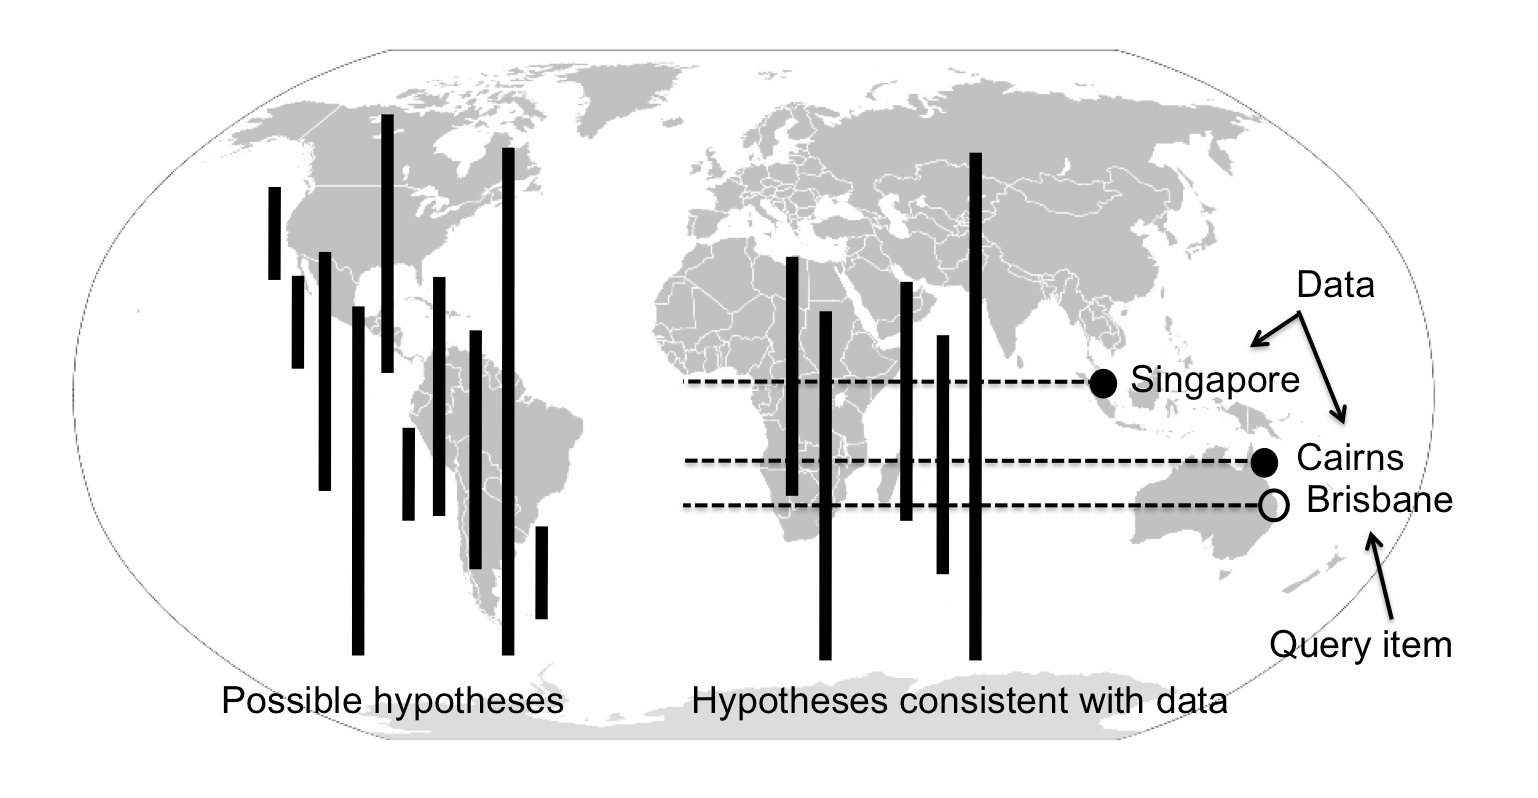
\epsfig{file=./figs/tropics.eps,width=11cm}
\caption{A schematic illustration of the tropics example, showing a collection of possible hypotheses (left), a data set and novel query items (right), and showing how only some of the hypotheses are consistent with the data (middle).}
\label{tropics}
\end{center}
\end{figure}

As noted by \citeA{Tenenbaum2001}, the theory extends to multiple examples in a very simple way. We now imagine that the learner has encountered $n$ items that possess the property, corresponding to the observations $\bm{x} = (x_1,\ldots,x_n)$. In this situation, the learner knows that the items $\bm{x}$ have been generated, and also knows that these items belong to the true consequential region, $\bm{x} \in \rt$. If we suppose that the items are conditionally independent\footnote{In view of our discussion about correlated environments, this assumption may seem odd. However, it is important to recognize that {\it conditional} independence is not inappropriate: part of the qualitative idea behind the mixed sampling model is to use $\theta$ to express the dependencies among items. That is, with probability $\theta$ the generation of observation $x$ may be deemed to be formative, but is otherwise deemed to convey no new information.} and apply Bayes' rule, we obtain the expression
\begin{eqnarray}
P(\rt = r \condon  \bm{x}, \bm{x} \in \rt) &\propto& P(\bm{x}, \bm{x} \in \rt \condon  \rt = r) \pgap P(\rt = r) \\
&=& \left( \prod_{i=1}^n P(x_i, x_i \in \rt \condon  \rt = r) \right) P(\rt = r).
\end{eqnarray}
Given the simplicity of this expression, multiple items may be handled easily. Moreover, since it is constructed from the same two functions (the prior and the likelihood), there is nothing conceptually different about the multiple item case. Again, noting that the likelihood is zero for any region $r$ that does not contain all of the training items $\xn$, one part of the learning process is to eliminate all hypotheses that are inconsistent with the data. To continue with the ``tropics'' example earlier, the learner might be told that Cairns (latitude $-16.9^\circ$) and Singapore (latitude $1.3^\circ$) lie in the tropics. On the basis of this knowledge, many of the originally possible regions are eliminated, as illustrated on the right hand side of Figure~\ref{tropics}.

\subsection{Making predictions}

When solving an inductive generalization problem, the learner's task is slightly more complex. Rather than needing to infer the true consequential region associated with the property, the learner needs to determine if some novel item $y$ also shares the property. In the tropics example, this might correspond to a situation in which the learner has been told that Cairns and Singapore lie in the tropics, and is asked to guess if Brisbane (latitude $-27.4^\circ$) also lies in the tropics. Formally, the problem at hand is to infer the probability that $y \in \rt$ given that the learner has observed $\xn$ and knows that $\xn \in \rt$. Clearly, if the identity of the true region is known to the learner then this problem becomes trivial. However, the learner does not have this knowledge. Instead, what the learner has is a set of beliefs about the plausibility of different regions, as captured by $P(\rt = r \condon  \bm{x}, \bm{x} \in \rt)$ as discussed earlier. If the learner weights each hypothesis according to its probability of being correct, then he or she can infer that the probability that the new item also possesses the property, as follows:
\begin{equation}
\p(y \in \rt \condon  \bm{x}, \bm{x} \in \rt) =  \int_{\mathcal{R}} \p(y \in \rt \condon  \rt=r) \pgap \p(\rt=r \condon  \bm{x}, \bm{x} \in \rt) \ dr. \label{aaa}
\end{equation}
In this expression the $\p(y \in \rt \condon  \rt=r)$ term is very simple: it is just the ``probability'' that $y$ falls inside some known region $r$. Therefore, it equals 1 if $y$ is inside this region and 0 if it is not. Not surprisingly then, only those regions that include $y$ make any contribution to the integral in Equation~\ref{aaa}, and so we can simplify this expression by restricting the domain of the integration to $\mathcal{R}_y$, the set of regions that contain $y$. Thus we may write
\begin{equation}
\p(y \in \rt \condon  \bm{x}, \bm{x} \in \rt) =  \int_{\mathcal{R}_y}\p(\rt=r \condon  \bm{x}, \bm{x} \in \rt) \ dr, \label{genint}
\end{equation}
As noted earlier, the solution to this integral is presented in the Appendix for all cases relevant to this paper. However, in order to understand the behavior of the model, it suffices to note that all this integral does is ``add up'' the total degree of belief associated with those regions that include $y$. To return again to our tropics learning example in Figure~\ref{tropics}, there are five hypotheses that are consistent with the training data (Singapore and Cairns). Of those five hypotheses, four also contain the query item (Brisbane). Therefore, if the learner treats all five of these hypotheses as equally likely, he or she would rate the probability of Brisbane being tropical at 80\%. Of course, in the actual model the learner's hypothesis space consists of all possible regions, not just the ten shown in the Figure, but the basic principle is the same: the learner generalizes using only those hypotheses that are consistent with the data. The more important issue is whether the learner would really treat all of the data-consistent hypotheses as equally plausible. To answer that question, we must now look at the priors and the likelihoods in detail.


\subsection{Priors and likelihoods}

To complete the model, we need to specify $P(\rt = r)$, the learner's prior degree of belief in region $r$, and the likelihood function $P(x, x \in \rt \condon  \rt = r)$. As discussed earlier, the family of likelihood functions that we consider in this paper are those that correspond to the ``mixed sampling'' model (Equation~\ref{miiixed1}). In order to do so we may (without loss of generality) assume that the range $\mathcal{X}$ over which stimuli can vary is the unit interval, $[0,1]$. In the tropics example, for instance, we can do this by dividing the latitude by 180 and then adding 0.5. In these new co-ordinates, the tropics correspond to the region that runs from $0.37$ to $0.63$. Having made this assumption, the mixed sampling likelihood functions are given by
\begin{equation}
\p(x, x \in \rt \condon  \rt=r, \theta) = \left\{ \begin{array}{cl} (1-\theta) + \theta\displaystyle\frac{1}{|r|} & \mbox{ if } x \in r \\ 0 & \mbox{ otherwise} \end{array} \right.. \label{miiixed}
\end{equation}
where $|r|$ denotes the size of the region, and as discussed previously $\theta=0$ yields the weak sampling model and $\theta=1$ is the strong sampling model. In these normalized co-ordinates, therefore, the size of the tropics is $0.63 - 0.37 = 0.26$.


What degree of prior belief should the learner place in the hypothesis that region $r$ is the correct one? One natural possibility is the uniform prior, $P(\rt = r) \propto 1$, in which the learner treats every possibility as equally likely. However, this is not the only possibility that the learner might consider. Consider the region $r$ that covers the interval $[l,u]$. The size of this region is given by $|r| = u-l$, and the location of this region is the center $c=(u+1)/2$. In keeping with \citeA{Shepard1987} we assume that it is only the size of a region that matters, not its location. With this in mind, one natural choice of prior is the simple one-parameter Beta$(1,\phi)$ model, in which
\begin{equation}
 \p(\rt=r) \propto |r|^{\phi-1}.
\end{equation}
Although simple, this prior is quite principled. It has the same structure as the likelihood function (i.e., size raised to some power), which means that $\phi$ can be interpreted as pseudo-data. That is, increasing $\phi$ by one has exactly the same effect on the generalization function as decreasing the sample size by one. In other words, if the learner's pre-existing knowledge can be described ``as if'' it corresponded to a set of fictitious previous observations, then the prior distribution should take this form. The result is a family of priors in which $\phi=1$ corresponds to a uniform distribution over possible regions, whereas $\phi<1$ expresses a prior assumption that the region is small, and $\phi>1$ corresponds to a prior belief that the region extends over a larger range. To illustrate this idea, Figure~\ref{tropicsprior} shows the prior distribution that would be involved in the tropics example, if the 10 hypotheses shown in Figure~\ref{tropics} were in fact the entire hypothesis space. When $\phi = 1$ (middle panel), all regions are treated as equally plausible a priori. A prior that is biased towards small regions ($\phi=0.5$) is shown in the left panel, while the right panel depicts a bias towards larger regions ($\phi=2$).

\begin{figure}
\begin{center}
\begin{tabular}{ccc}
\hspace*{-.65cm}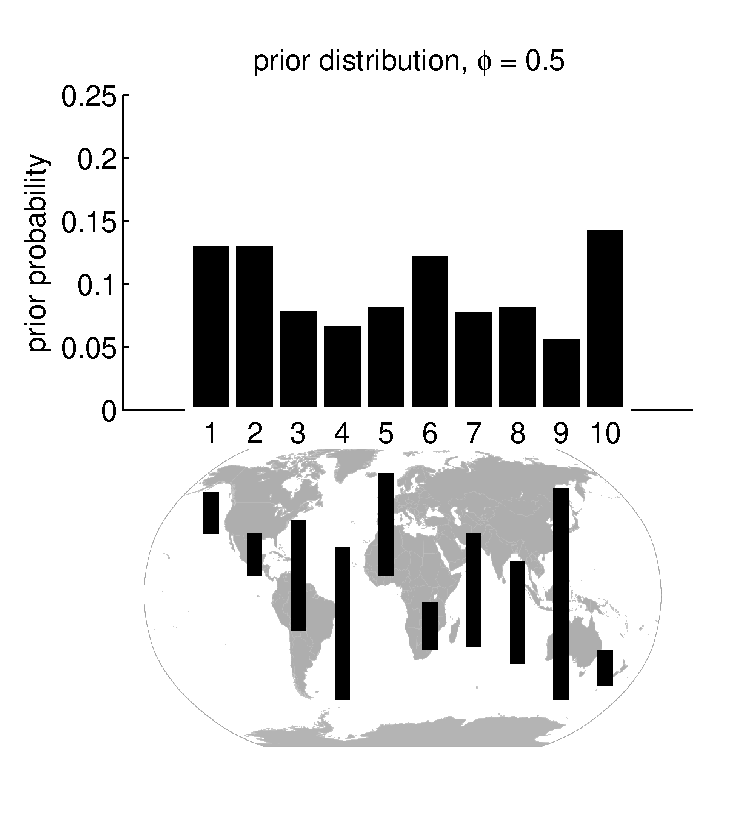
\epsfig{file=./figs/tropicsprior1.eps,width=5.5cm} &
\hspace*{-.65cm}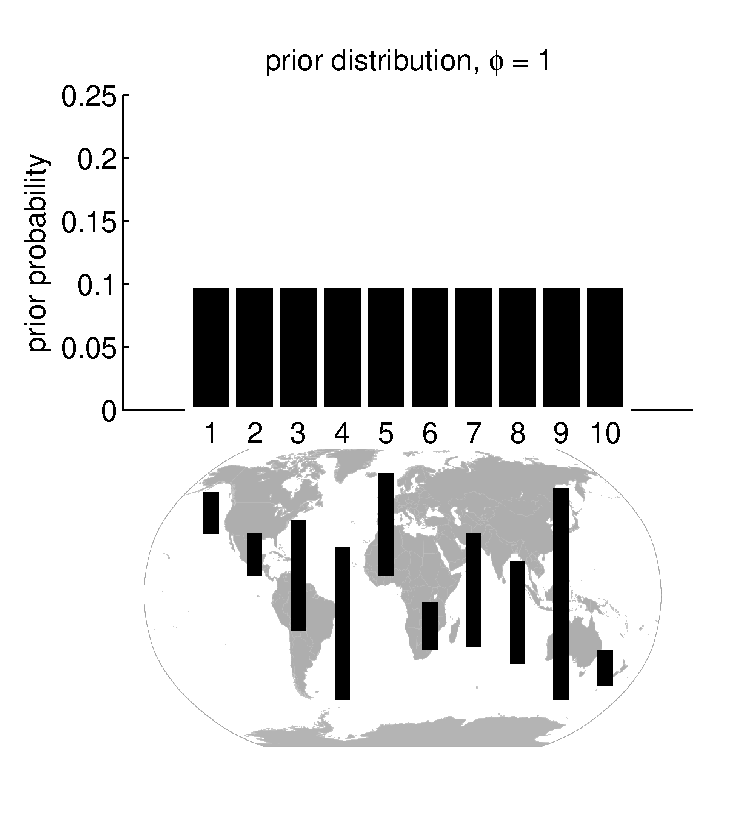
\epsfig{file=./figs/tropicsprior2.eps,width=5.5cm} &
\hspace*{-.65cm}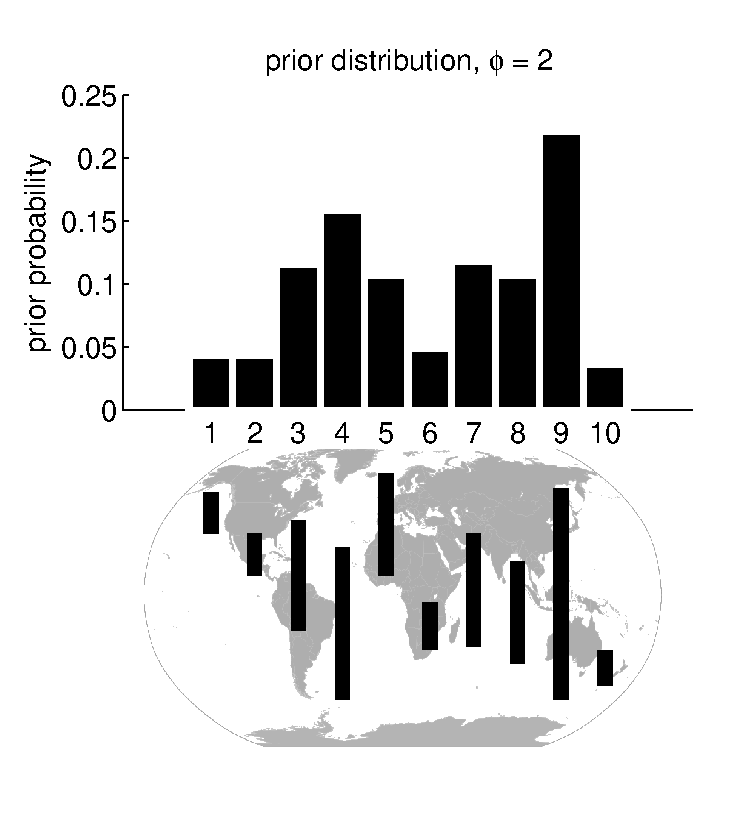
\epsfig{file=./figs/tropicsprior3.eps,width=5.5cm}
\end{tabular}
\caption{The tropics prior. Lower panels show 10 different hypotheses the learner might have regarding how far the tropics extend. The top panels plot the prior degree of belief that a learner might have, depending on the value of $\phi$.}
\label{tropicsprior}
\end{center}
\end{figure}


\begin{figure}
\begin{center}
\begin{tabular}{ccc}
\hspace*{-.65cm}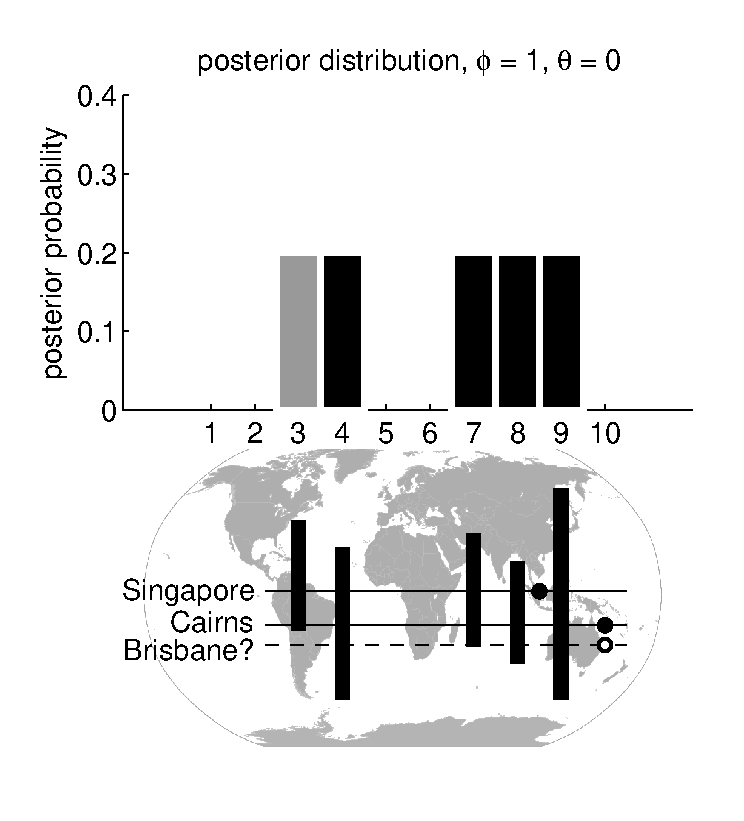
\epsfig{file=./figs/tropicsposterior1.eps,width=5.5cm} &
\hspace*{-.65cm}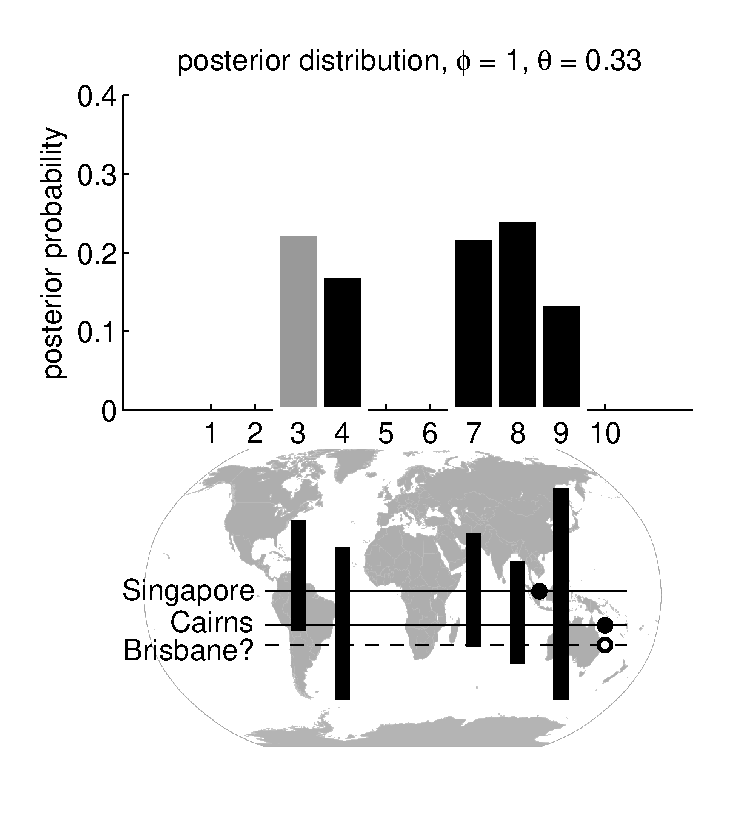
\epsfig{file=./figs/tropicsposterior2.eps,width=5.5cm} &
\hspace*{-.65cm}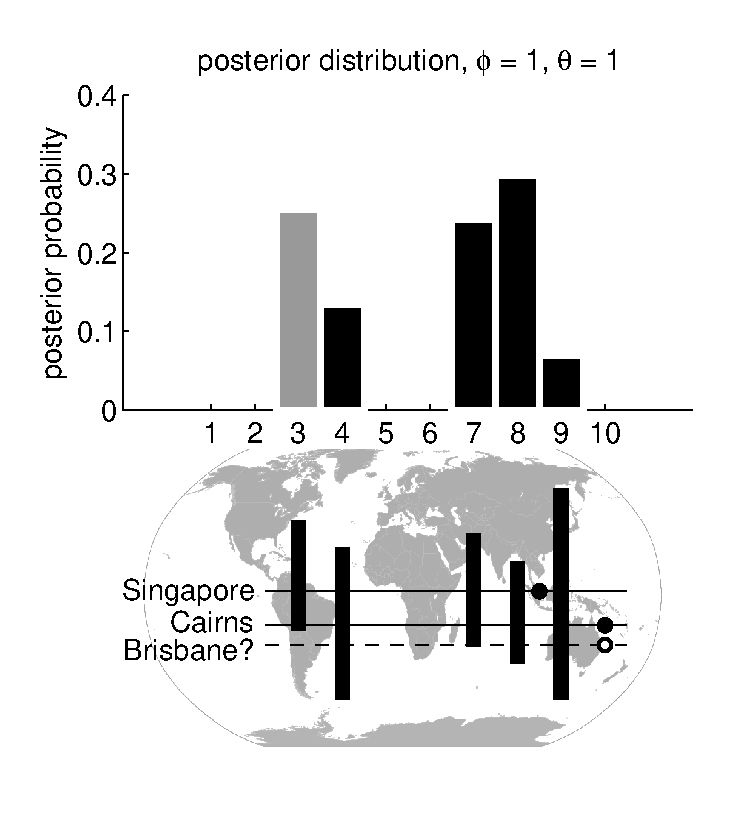
\epsfig{file=./figs/tropicsposterior3.eps,width=5.5cm}
\end{tabular}
\caption{The tropics posterior. Lower panels show 5 hypotheses that are consistent with the observed data (i.e., the fact that Singapore and Cairns are both tropical), while the upper panels show the posterior degree of belief that the learner might have, depending on the sampling assumptions $\theta$ (assuming that $\phi = 1$). The black bars depict hypotheses that would predict Brisbane to be tropical as well, while the grey bars correspond to the hypothesis that predicts Brisbane not to be tropical.}
\label{tropicsposterior}
\end{center}
\end{figure}

Now that we have both the prior and the likelihood specified, the influence of the sampling assumptions $\theta$ can be made explicit. Figure~\ref{tropicsposterior} plots three posterior distribution for the tropics problem, where the prior distribution is assumed to be uniform (as per the middle panel of Figure~\ref{tropicsprior}), using a weak sampling model ($\theta=0$), a strong sampling model ($\theta=1$) and an intermediate model ($\theta=.33$). Note that the pattern of falsification is the same in all three cases: regardless of the value of $\theta$, hypotheses 1, 2, 5, 6 and 10 are all inconsistent with the data, because the corresponding regions do not contain both Singapore and Cairns. Thus the posterior probability for these regions is zero. In weak sampling (left panel), this is the only change from the prior distribution, and so the five remaining hypotheses are equally weighted. Since the only one of the remaining hypotheses not to contain Brisbane is hypothesis 3 (shown in grey), in this case the learner would say that there is an 80\% chance that Brisbane lies in the tropics. However, if $\theta>0$ then the likelihood favors the smallest regions that are consistent with the data (i.e., contain Singapore and Cairns). Thus, the likelihood will always favor hypothesis 8 most strongly, followed by hypotheses 3, 7, 4 and 9 in that order. When $\theta$ is near 1, this effect is very strong (right panel of Figure~\ref{tropicsposterior}) whereas for $\theta$ close to 0 this effect is much smaller. As a result, when $\theta=.33$ the learner's estimate of the probability that Brisbane is tropical falls to 77\%, which drops to 75\% when $\theta=1$.

\subsection{Constructing a Generalization Gradient}

Up to this point, the tropics example that we have used to illustrate model behavior has relied on an ad hoc hypothesis space consisting of only 10 possible consequential regions. Moreover, we have only examined the model predictions for a single query item (i.e., Brisbane, latitude $-24.4^\circ$). However, in order to understand the overall behavior of the model, we need to remove both of these restrictions. To start with, suppose we expanded the hypothesis space to include all regions where the edge points are a member of the set $.05, .15, \ldots, .85, .95$ (that is, a very crude discrete approximation to $\mathcal{R}$). Using this expanded hypothesis space, we can then calculate the posterior distribution over possible regions $P(\rt = r \condon \xn, \xn \in \rt)$ for different choices of the two parameters $\theta$ and $\phi$, as well as the generalization probability $P(y \in \rt \condon \xn, \xn \in \rt)$ for all possible query items $y$.

In the simplest case, suppose the learner has a uniform prior over regions $\phi = 1$ and applies a weak sampling model $\theta = 0$. This case is illustrated in the left panels of Figure~\ref{discreteexample}. The lower part of the plot draws all of those regions that are consistent with the two observations (Singapore and Cairns). Since all of these regions were equally likely in the prior, and the weak sampling likelihood function {\it only} acts to falsify regions that do not contain the data, all of these regions remain equally likely in the posterior (illustrated schematically by the fact that all of the lines are of the same thickness). In the top part of the panel, we plot the generalization probability $P(y \in \rt \condon \xn, \xn \in \rt)$ for all possible latitudes of the query item $y$. Since all of the regions in the lower panel are weighted equally, for any given value of $y$ this probability is just a count of the proportion of non-falsified regions that contain the query item.

When we use other parameter values, it is no longer the case that all regions are equally likely. For instance, suppose the learner switched from a weak sampling model to a strong sampling model, by increasing $\theta$ from 0 to 1. It is now the case that the likelihood function strongly favors the {\it smallest} regions that contain both Singapore and Cairns. This situation is shown in the middle panel of Figure~\ref{discreteexample}. The lower part of the plot schematically illustrates the effect of the likelihood on the posterior distribution over regions: smaller regions are more likely, and are thus drawn with thicker lines. The upper panel shows what effect this has on the generalization gradient: it ``tightens'' around the data, because the narrowest regions are preferred by the learner.

The right hand panel of Figure~\ref{discreteexample} shows what influence the prior has, by raising $\phi$ from 1 to 5. By choosing a prior with $\phi = 5$, the learner has a prior bias to believe that the region is large (i.e., that the tropics covers a very wide band of latitudes). Even though the learner has a weak sampling likelihood function (i.e., $\theta = 0$) the posterior distribution in the lower panel is quite uneven, as a result of the learner's prior biases. In this case, because the prior bias was to favor large regions, the effect of the generalization gradient is the opposite of the effect we observed in the middle panel: the generalization gradient spreads out, and in fact becomes convex.

One critical implication of this phenomenon should be made explicit: the effects of $\phi$ and $\theta$ are very similar if we consider only a single generalization gradient. That is, raising $\theta$ has the same effect as reducing $\phi$. Indeed, this is a general property of Bayesian models. In order to disentangle the influence of the learner's prior beliefs ($\phi$) from their assumptions about data ($\theta$) it is necessary to look at how the overall pattern of generalizations changes across {\it multiple} generalization gradients.


\begin{figure}
\begin{center}
\begin{tabular}{ccc}
\hspace*{-.65cm}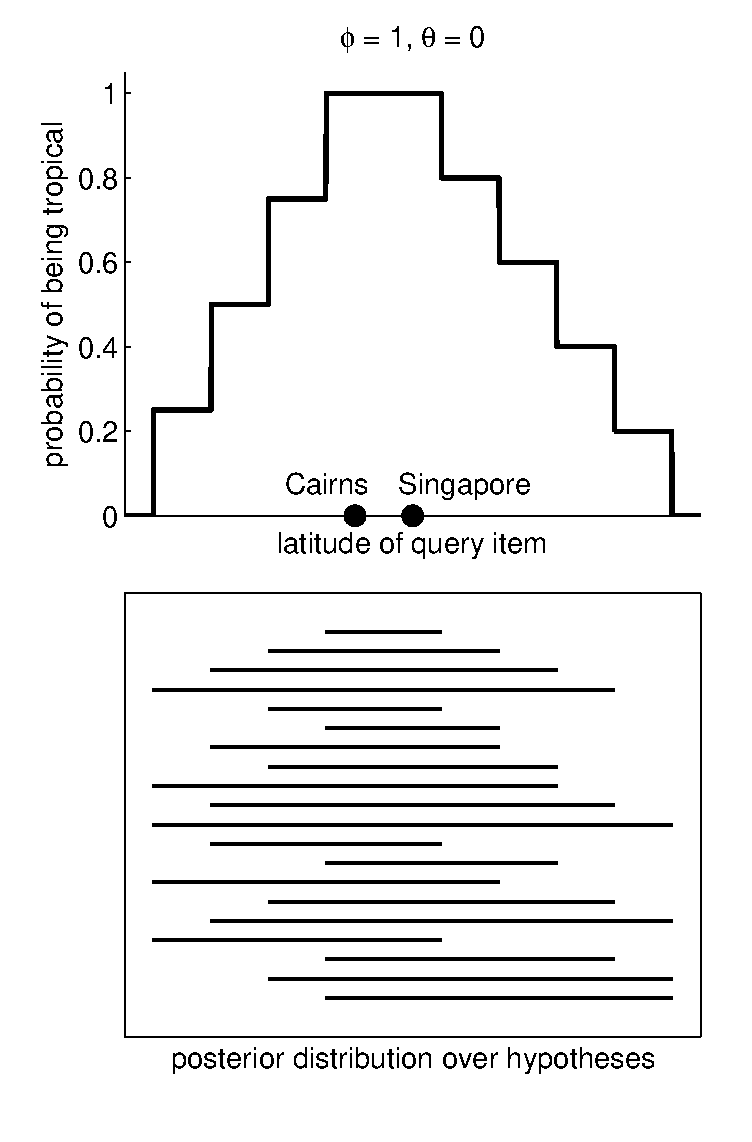
\epsfig{file=./figs/discreteexample1.eps,width=5.5cm} &
\hspace*{-.65cm}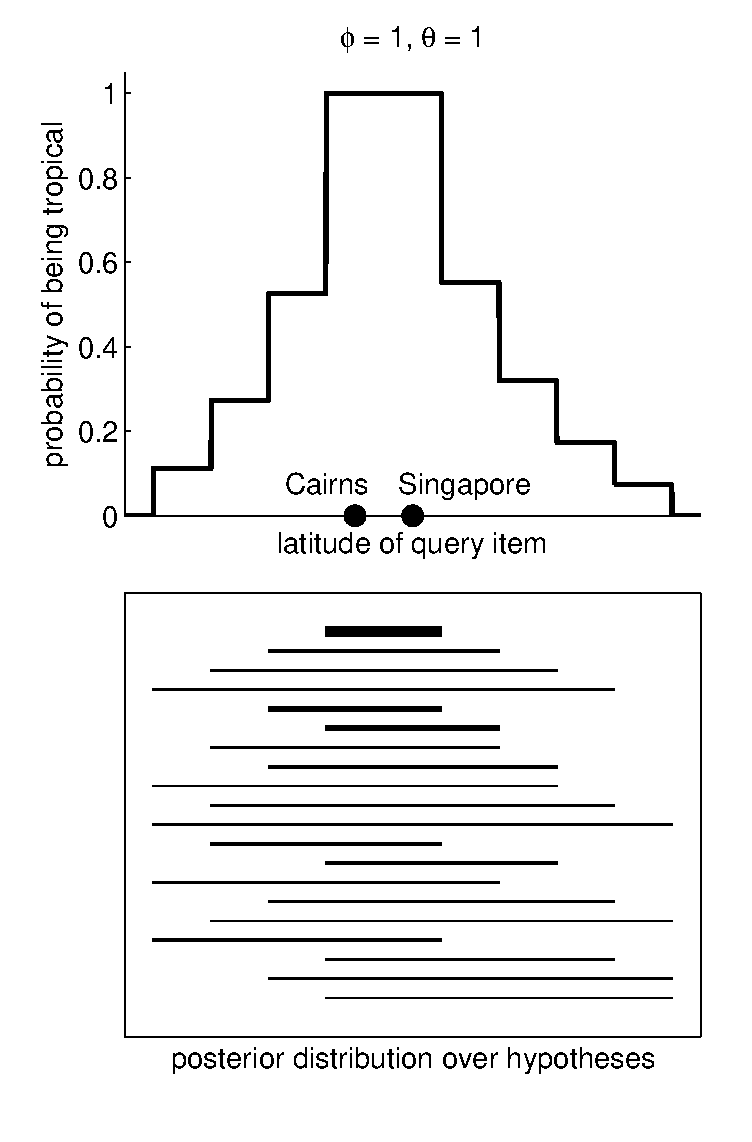
\epsfig{file=./figs/discreteexample2.eps,width=5.5cm} &
\hspace*{-.65cm}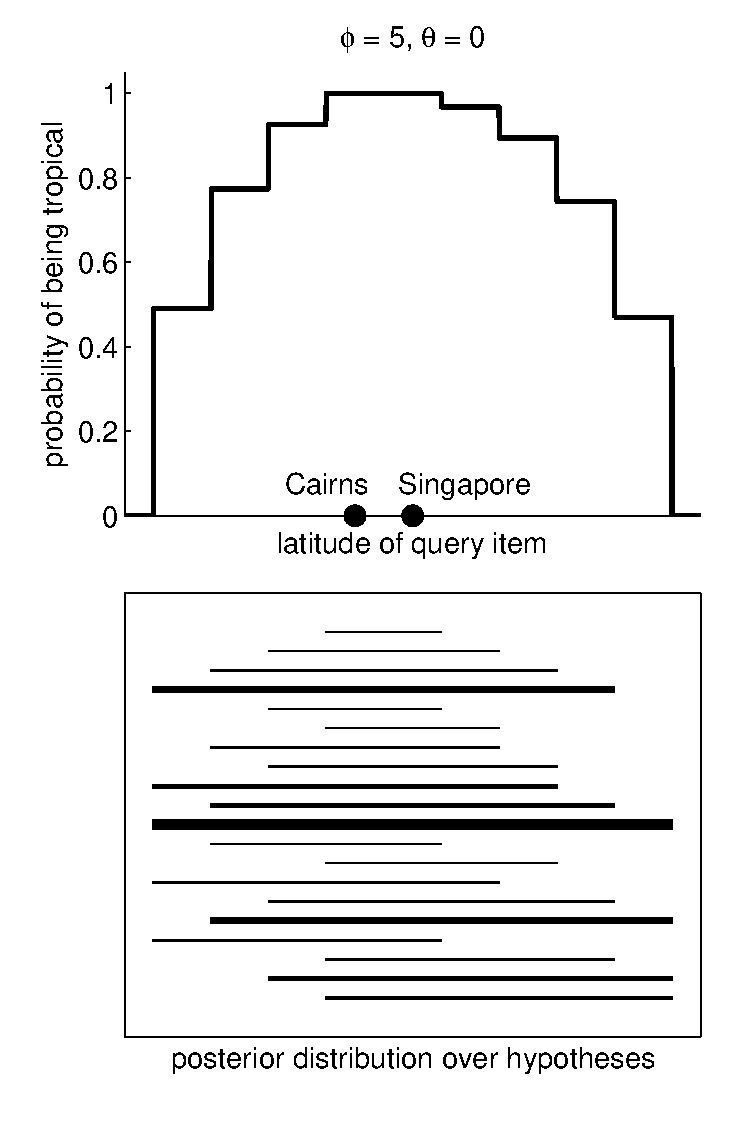
\epsfig{file=./figs/discreteexample3.eps,width=5.5cm}
\end{tabular}
\caption{Construction of the generalization gradients. The lower three panels show a collection of hypotheses that are consistent with the training data in the tropics problem (i.e., Cairns and Singapore), where the width of each line illustrates the degree of belief that the learner has in that hypothesis. The generalization gradients at the top are constructed by calculating the probability of being tropical for all possible query items, as a function of their latitude. The differences between the plots arise due to differences in sampling models and priors.}
\label{discreteexample}
\end{center}
\end{figure}

Obviously, the stepped generalization functions shown in Figure~\ref{discreteexample} are not psychologically plausible. This lack of smoothness is an artifact of limiting the hypothesis space to a discrete approximation. If we expand the hypothesis space to consist of all possible regions, the problem becomes continuous, as do the corresponding generalization gradients. In the Appendix, we present solutions to the integrals involved in the continuous case, allowing us to directly calculate smooth generalization gradients rather than relying on numerical approximations.

\subsection{Generalization Gradients in the Full Model}

Having illustrated how the model predictions are constructed, we now turn to a discussion of what kinds of generalization patterns can be produced by varying the prior (via $\phi$) and the likelihood (via $\theta$). Of the two parameters, the one in which we are interested is $\theta$, but it is important to show how to disambiguate the two. To do this, consider what happens to the generalization gradients when the learner makes three observations, but sees them one at a time. For simplicity, assume that $\phi =1$ so the learner treats all regions as equally plausible a priori. The generalizations that are possible in this situation are illustrated in Figure~\ref{varytheta}. In the weak sampling case, the generalization gradients are linear and do not tighten.\footnote{The linearity may seem surprising, since Shepard's \citeyear{Shepard1987} analysis produced exponential gradients: the difference is partly due to the priors and partly due to the restriction to finite range.} Critically, notice that for any $\theta>0$ the generalization gradients get tighter as more data are observed (from left to right). As will become clear when we discuss the priors, this is the critical prediction -- the nonlinear shapes of the gradients in the lower panels can easily be mimicked by weak sampling if we choose the priors in the right way, but the tightening from left to right cannot. This is illustrated in Figure~\ref{varyphiweak}, which shows what happens when we vary $\phi$ (while keeping $\theta$ fixed at 0). The prior cannot influence the manner in which generalizations {\it change} as a function of data. It is this critical regularity that we seek to investigate experimentally.

\begin{figure}
\begin{center}
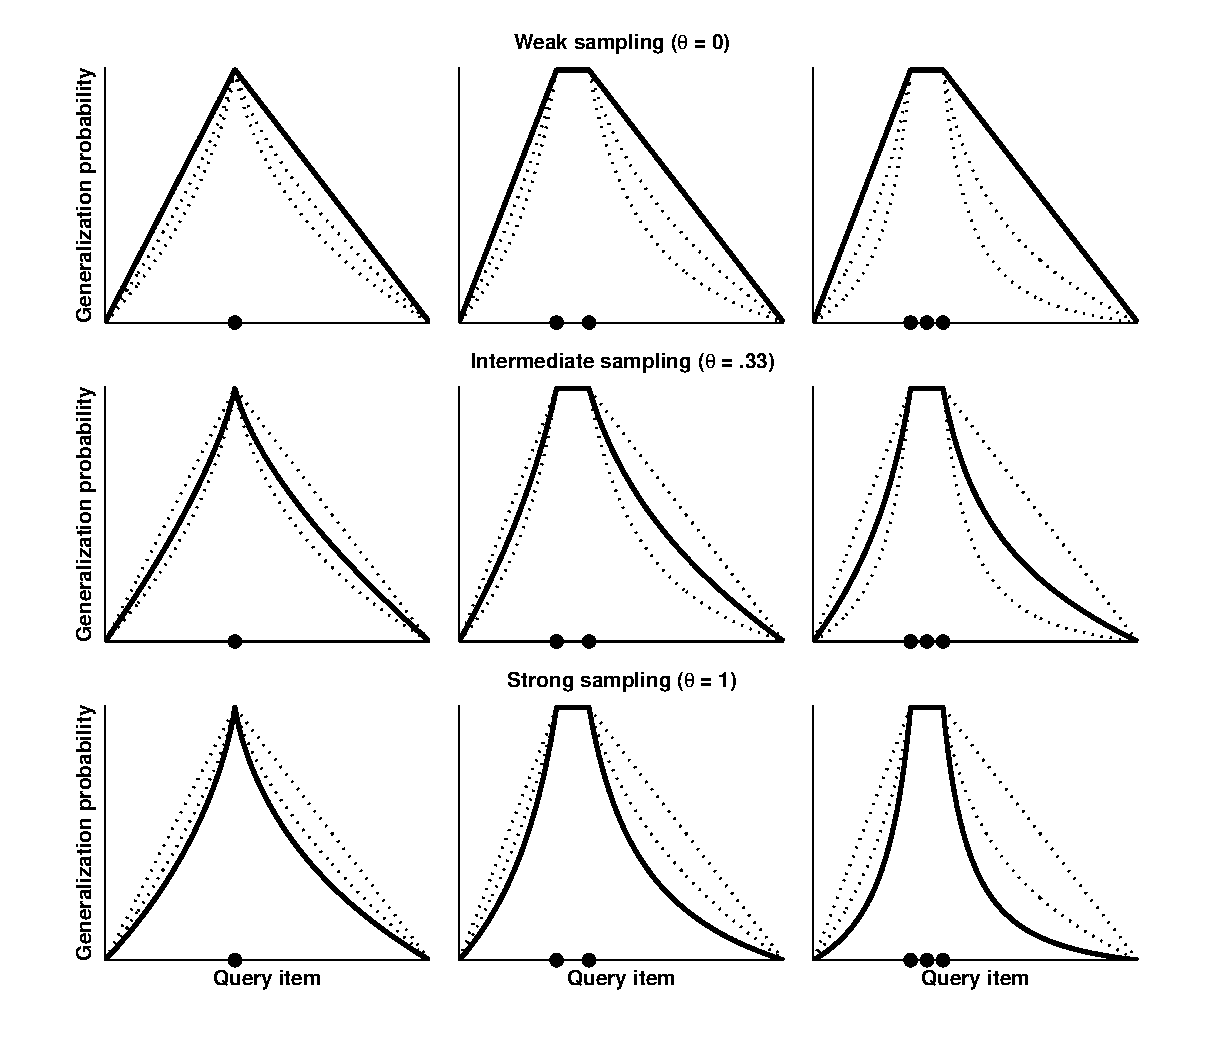
\epsfig{file=./figs/samplingmodelvariation.eps,width=13cm}
\caption{The effect of varying the sampling model $\theta$, for a situation in which the learner places uniform priors over all possible connected regions that contain the training items. The top panels show the weak sampling case ($\theta=0$), with the three panels showing the situation when the learner has observed one, two and three training items respectively. Note that in the weak sampling case, the generalization gradients do not tighten. In contrast, the middle panel shows an intermediate case ($\theta=.33$) while the lower panel shows the strong sampling case ($\theta=1$); in both cases the gradients get steeper from left to right. Note also that including some strong sampling in the mixture has a clear effect, in the sense that the curves for $\theta=.33$ are more similar to those for $\theta=1$ than they are for $\theta=0$.}
\label{varytheta}
\end{center}
\end{figure}

\begin{figure}
\begin{center}
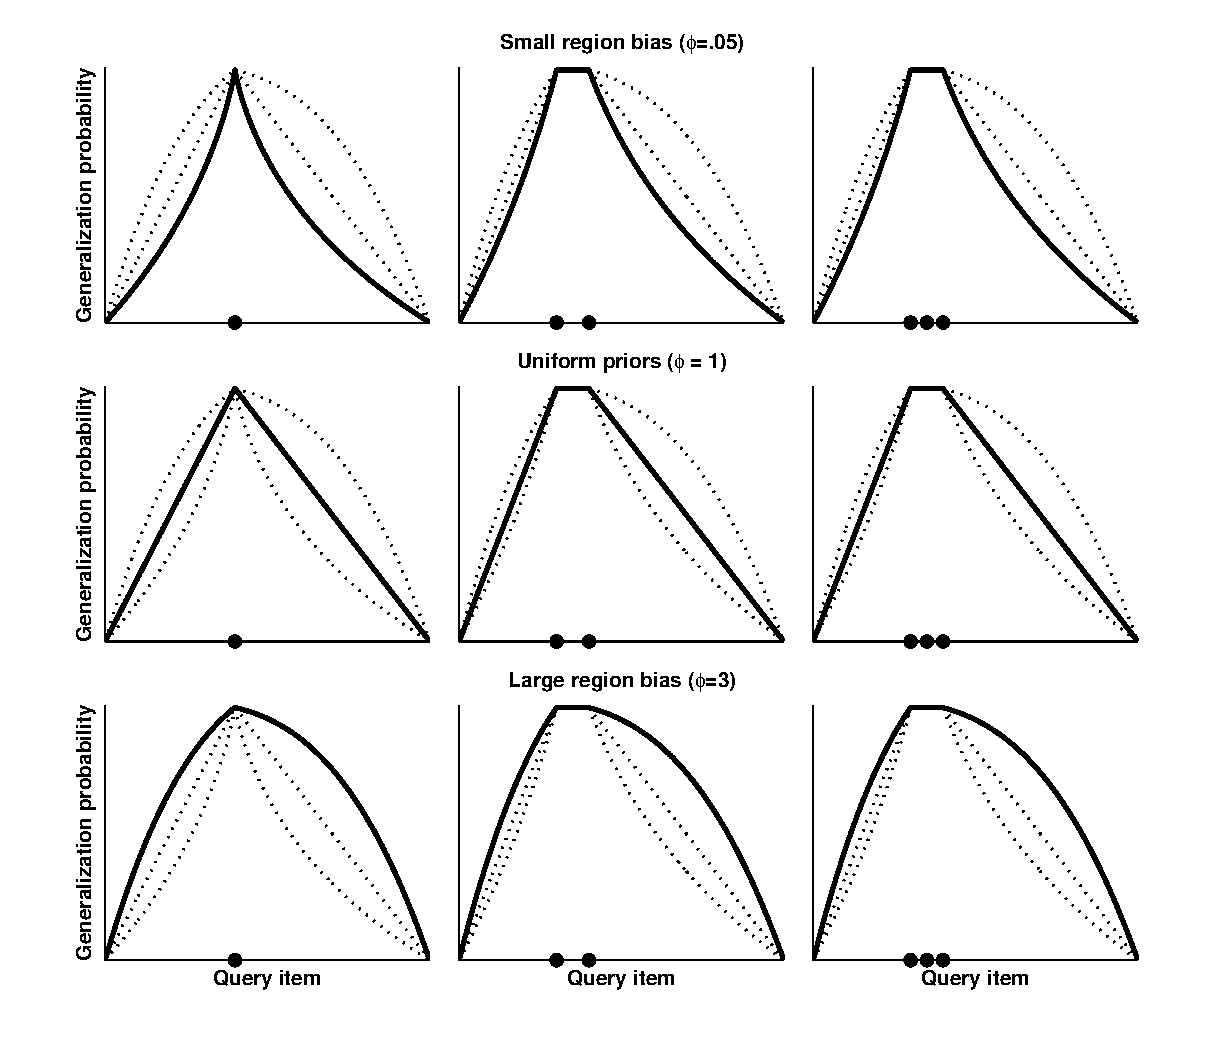
\epsfig{file=./figs/priorvariation.eps,width=13cm}
\caption{The effect of varying $\phi$, when the sampling model is weak ($\theta=0$) for a case involving three training items (black dots). The middle row shows the case where the prior is uniform ($\phi=1$), and is thus identical to the top row in Figure~\protect\ref{varytheta}. The top row shows a situation where the learner has a prior bias to expect the region to be small ($\phi=.05$), yielding convex gradients that look very similar to those observed in the lower panels of  Figure~\protect\ref{varytheta}. The bottom row, on the other hand, shows what happens when the learner has a prior bias to believe that the region will be large: the generalization gradients become concave.}
\label{varyphiweak}
\end{center}
\end{figure}

\section{Experiment One}

The question we want to investigate in this experiment is the extent to which people change their generalizations as a function of the number of observations they make. According to the weak sampling hypothesis \cite<as per>{Shepard1987,Heit1998,Kemp2009}, the generalization gradients should not tighten purely because more data are available. In contrast, the strong sampling hypothesis \cite<as per>{Tenenbaum2001,Sanjana2003} implies that the generalization gradients should narrow as data arrive, even if the new observations fall within the same range as the old ones.

\begin{figure*}[t]
\begin{center}
\hspace*{-1.2cm}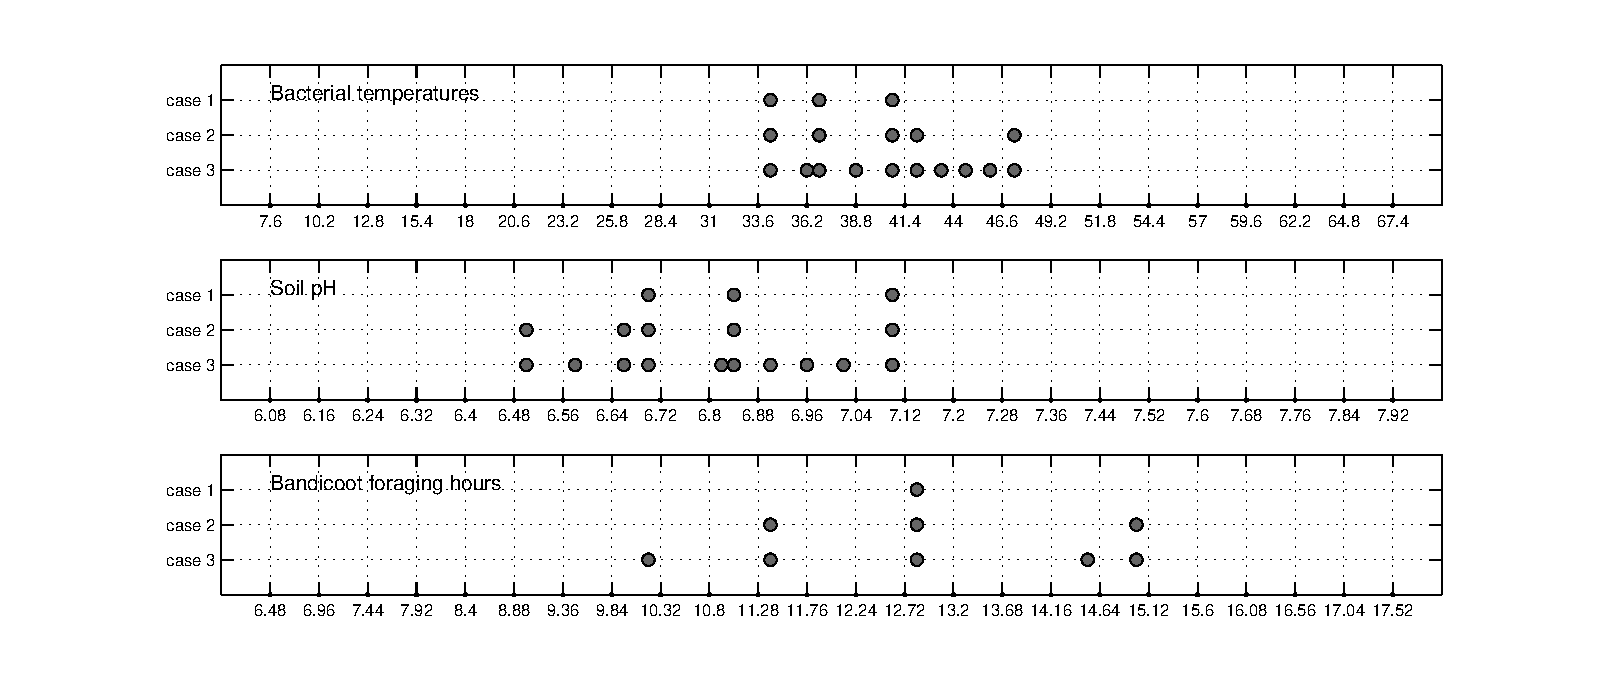
\epsfig{file=./figs/design2.eps, width=18cm}
\caption{The experimental design. Each panel corresponds to one of the three scenarios, and shows the three different sets of stimuli known to possess the property. The tick marks are located at each of the test points. See main text for details.}
\label{design}
\end{center}
\end{figure*}

\subsection{Method}

\subsubsection{Participants} Participants were twenty-two undergraduates (16 female, 6 male) from the University of Adelaide, who were given a \$10 book voucher for their participation.

\subsubsection{Materials \& Procedure} Participants were asked about three different induction problems, presented in a random order via computer. All problems involved stimuli that varied along one continuous dimension. One problem involved the temperatures at which a bacterium can survive, another asked about the range of soil acidity levels that produce a particular colored flower, and the third related to the times at which a nocturnal animal might forage. The cover story then explained that a small number of ``training'' observations were available -- in the bacterial scenario, for instance, it would indicate temperatures at which the bacterium was known to survive -- and asked participants to make guesses about whether or not the property generalized to different stimulus values (the ``query'' items).  The cover stories are provided in the Appendix.

To minimize any differences between the psychological representation of the stimuli and the intended one, participants were shown a visual representation of the data, which marked the locations of training items with a black dot, and the query item was shown using a red question mark. The cover stories were constructed to imply that the to-be-inferred property did not hold for beyond the range shown on screen. Responses were obtained by allowing people to position a slider bar using the mouse, with response values ranging from 0\% probability to 100\% probability. Once the participant was satisfied with the positioning of the slider bar, they clicked a button to move to the next question. For every set of training data, we presented 24 query items, spread evenly across the range of possible items and presented in a random order.

Since it is impossible to infer the sampling model from a single generalization gradient, we measured three generalization gradients for each problem, as illustrated in Figure~\ref{design}. Initially, participants were asked to make generalizations from a small number of observations. These were then supplemented with additional observations, and people were asked to generalize from this larger sample. Finally, the data set was expanded a third time to allow us to measure a third generalization gradient. In effect, we present people with three samples---collectively referred to as a ``data structure''---and obtain the corresponding generalization gradients. The assignment of cover stories (bacterial, soil, foraging) to data structures was fixed rather than randomized, as illustrated in Figure~\ref{design} (we address this in experiment two). For example, the top panel shows the data structure associated with the bacterial cover story. Each of the three rows corresponds to the three samples: three known observations were initially given, which was then expanded to five data points, and then finally to a sample of ten observations. In total, each participant made 216 judgments (3 scenarios $\times$ 3 samples $\times$ 24 queries).

\subsection{Basic Results}

\begin{figure}[t]
\begin{center}
\begin{tabular}{c}
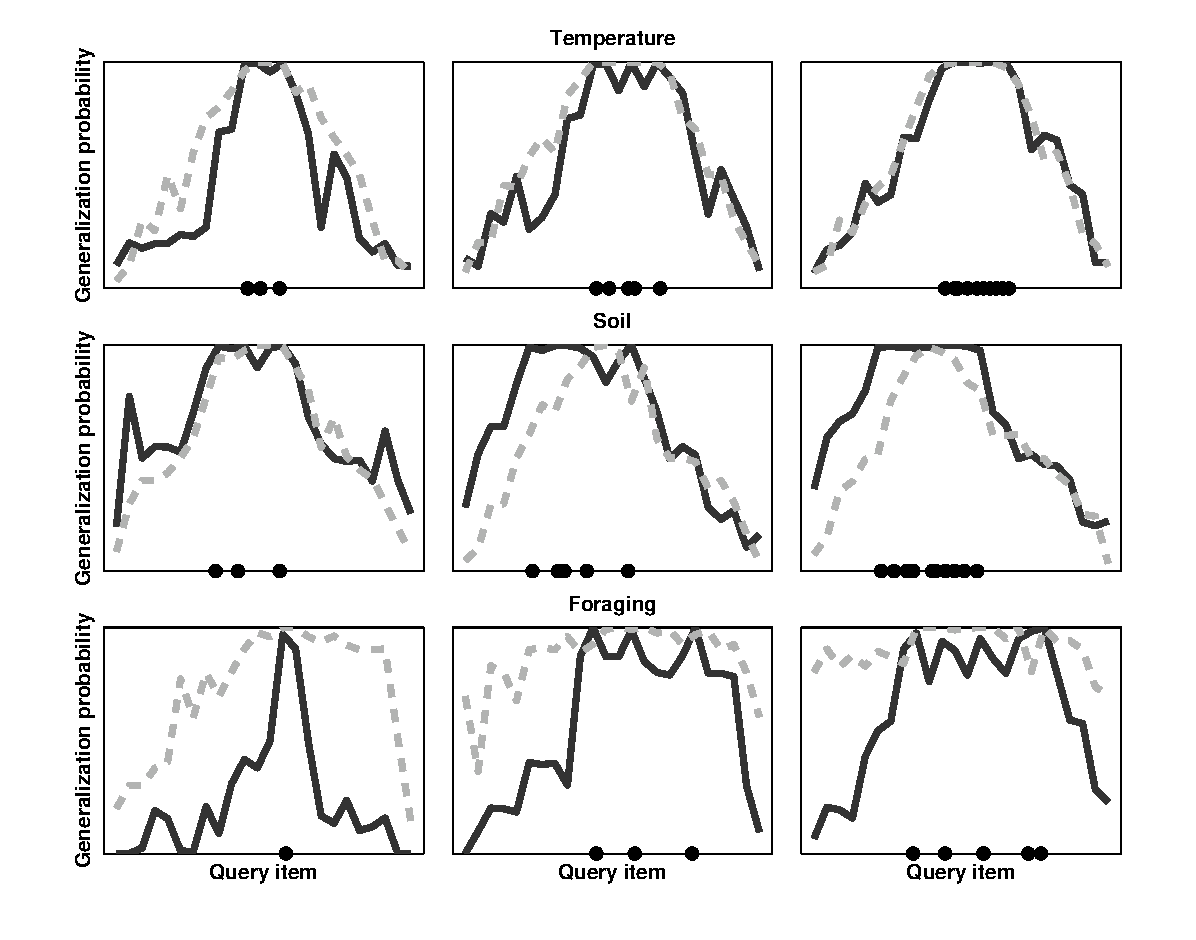
\epsfig{file=./figs/rawdata_participant14and2expt1.eps, width=13cm}
\end{tabular}
\caption{All 216 judgments made by participant 14 (dark solid lines) and participant 2 (light dashed lines). The gradients are all sensible, but the participants clearly differ from one another.}
\label{sampleraw}
\end{center}
\end{figure}

Figure~\ref{sampleraw} plots all 216 judgments made by two of the participants. In both cases the judgments appear sensible, but it is clear that the generalization gradients are quite different from one another. Indeed, inspection of the raw data across all 22 participants made clear that individual differences are the norm rather than the exception. With this in mind, in the model-based analyses we present later in this section we took care not to average data across participants. Moreover, later in the paper we examine the individual-level data in some detail. However, before modeling the data, we present some more basic analyses.



As discussed earlier, the basic effect that we are looking for is the ``gradient tightening'' effect shown in Figure~\ref{varytheta}. That is, do people narrow their generalization gradients as sample size increases? A simple way to test this proposition is to note that the experimental design is such that there are multiple occasions where more data are added to the sample, but at least one of the two edge points remains unchanged (Figure~\ref{design}). For instance, one of the seven cases corresponds to the transition from the first to second sample in the bacterial scenario: on the left hand side, the edge point does not change. To a first approximation, it is reasonable to assume that if $\theta>0$, the generalization probabilities should decrease for the query items that lie beyond this edge.\footnote{This is not strictly correct, insofar as the behavior of a strong sampling model can sometimes depend on what happens to both of the edge points, not just the nearest one. Even so, the results of this simple analysis are in accordance with the results of the more detailed model fitting presented later in the paper.}   In total, there are seven situations in which the edge point does not change, yielding a total of 64 pairs of queries.  Since there are 11 query items to the left of the leftmost training example in this instance, this contributes 11 of the 64 query pairs that we can consider, and thus a total of $22 \times 64 = 1408$ pairs of responses. For each such pair of queries, we are interested in the difference between generalization probabilities reported by each participant, since this provides a measure of the extent of ``gradient tightening.'' On average, people showed a small but significant amount of gradient tightening:  the generalization probabilities are lower on average when the sample size is larger ($t_{1407}=-4.98$, $p<.001$). Individually, the trend is the correct direction for 51 of the 64 query pairs, and for 17 of the 22 participants. However, notice that this a small effect: the raw judgments vary from a probability of 0\% to 100\%, but the average change corresponds to a decrease in generalization probability of only 2.3\% from one case to the next.



\subsection{Model-Based Analyses}

\begin{figure}[t]
\begin{center}
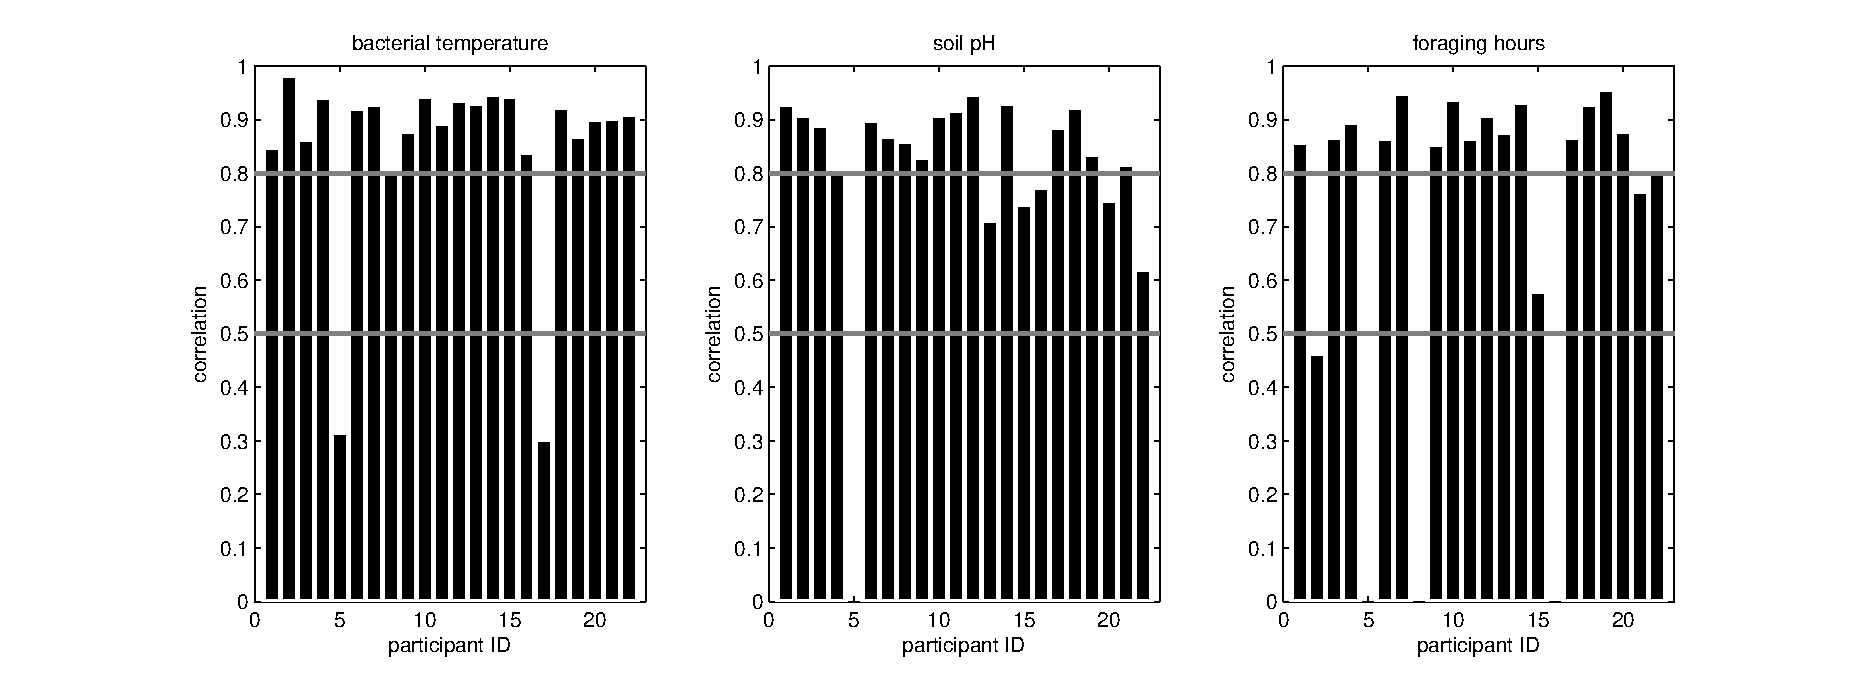
\epsfig{file=./figs/correlations1.eps,width=16cm}
\caption{Correlations between human data and model predictions in experiment 1, displayed for all 22 participants and all 3 scenarios. After making degrees-of-freedom corrections for the two extra free parameters ($\theta$ and $\phi$), there are 4 non-significant correlations among the 66 cases, involving participants 5 (scenarios 2 and 3) 8 (scenario 3) and 16 (scenario 16). These four cases are plotted as having a correlation of zero. Of the remaining 62 significant correlations, 61 are significant at the .001 level and 1 is significant at the .01 level. Grey bars plot the thresholds used to classify model performance as ``good'', ``moderate'' or ``poor''.}
\label{correl1}
\end{center}
\end{figure}


The simplified analysis in the previous section provides some evidence that the ``gradient tightening'' effect is present in these data, but the effect is quite weak, and leaves a great many questions unanswered. Is the tightening effect actually consistent with the strong sampling model proposed by \citeA{Tenenbaum2001}, or indeed with any of the sampling models discussed in this paper? Is the effect present for all scenarios, or only one or two? Do people tend to rely on the same sampling assumptions, or do people differ in this respect? In order to answer these questions, we need to fit the model to data explicitly. In this section we present an analysis that discusses two key questions: (1) the extent to which the Bayesian model successfully fits the data, and (2) what assumptions about $\theta$ are implied by these data. However, although we are careful not to average data across participants because of the individual differences that exist, we do not discuss these differences in any detail in this section: we return to this topic later in the paper.

The first question of interest relates to the adequacy of the generalization model. In order to address this question, we estimated the best fitting values of $\theta$ and $\phi$ separately for all 22 participants and all 3 scenarios, yielding a total of 66 parameter estimates (details are provided in the Appendix). We then measured the correlation between human responses and the model predictions at these best-fitting parameters, where the correlation is taken over the 72 judgments (24 queries $\times$ 3 cases) that each participant made in each scenario. Note that this set up means that the model needs to predict every single judgment made by every participant: no aggregation of data at any level is involved. The resulting correlations are plotted in Figure~\ref{correl1}. After making a degrees of freedom adjustment to account for the two extra free parameters (i.e., $\theta$ and $\phi$), almost all correlations (62 of 66) are significant. More importantly, the correlations are quite strong, especially in view of the fine grain at which we are modeling the data: the median correlation is 0.77, with an interquartile range of [.65, .85]. Overall, it is clear that the model is able to describe the data well.



\begin{figure}[t]
\begin{center}
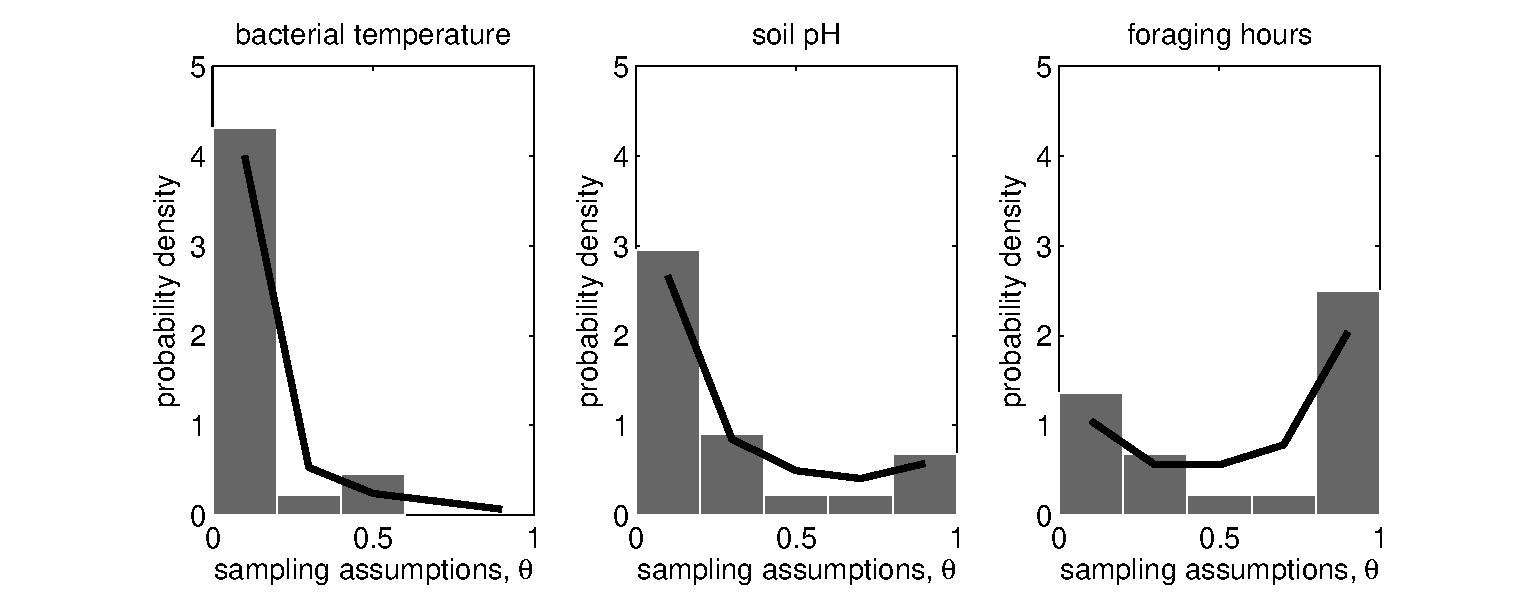
\epsfig{file=./figs/marginalposteriors_expt1.eps,width=15cm}
\caption{Distributions over $\theta$ observed in experiment 1. Each panel plots the distribution of best estimates (grey histograms) across the 20 participants, with each panel corresponding to one of the three scenarios. The black lines plot essentially the same analysis, but using the full posterior distributions over $\theta$ rather than just the best estimate for each participant. Reassuringly, the two versions of the analysis are in close agreement.}
\label{margpost1}
\end{center}
\end{figure}



Given that the model fits appear to be quite good, it is natural to ask what values of $\theta$ are involved. As the histograms in Figure~\ref{margpost1} illustrate, there is evidence for both strong sampling and weak sampling in this task. However, it is also there are clear differences between people and between scenarios. While the distributions are unimodal and biased towards weak sampling (small $\theta$) in two of the three scenarios,  the distribution of estimates for the foraging scenario is rather bimodal.


\subsection{Discussion}

The overall pattern of results to experiment one highlights several points. Firstly, there is quite strong evidence that the Bayesian generalization model is able to describe accurately the behavior of participants at a quite fine-grained level of analysis (prediction of every judgment in the experiment). However, it is important to take note of the technical literature that discusses how to  measure safely the adequacy of a model's performance, addressing issues such as model complexity \cite<e.g.>{Myung2000b,Pitt2002,Myung2006}, individual differences \cite<e.g.>{Lee2005b,Navarro2006a} and contaminant processes \cite<e.g.>{Huber1981,Ratcliff2002,Zeigenfuseinpress}. In fact, although we glossed over the details, our analysis does in fact accommodate all of these topics: the Appendix provides a discussion of how this was done.

Secondly, the data are quite informative as regards the default assumptions that people make about how observations are generated (at least in some contexts). Notice that the scenario descriptions did not explicitly state how the data were generated: participants were expected to supply the missing ``sampling'' assumption on their own. That said, there is a sense in which the data themselves suggest a strong sampling model, since participants only ever observed positive examples of a category. If people relied solely on this as a cue, then we would expect a bias towards larger values of $\theta$. Despite this, the reverse is true: on the whole, smaller values of $\theta$ tended to predominate.

Thirdly, the pattern of variation in the estimated $\theta$ values between scenarios is interesting. When the scenarios were originally designed we did not anticipate finding any differences between them: it was assumed that these differences would be presentational gloss and no more. Nevertheless, what we in fact observed is a relatively substantial difference in the distributions over $\theta$. People did seem to have a strong bias towards weak sampling in two of the scenarios, and a weak bias to prefer strong sampling in the third.

This third point deserves further investigation. Specifically, the fact that we found differences across the scenarios raises additional questions regarding the origin of these differences. In particular, we note that the ``foraging'' scenario (which induced larger $\theta$ values than the other two) differed from the other two problems in two respects. Firstly, as illustrated in Figure~\ref{design}, the changes in sample size involves an increase from 1 to 3 data points, and from 3 to 5 data points. In contrast, while the other two scenarios also have a jump from 3 to 5, the jump from 5 to 10 data points involves a smaller proportional increase (doubling) than the jump from 1 to 3 (tripling). One possible explanation for the use of strong sampling in this situation is that the ratios in the ``1:3:5'' structure are larger than in the ``3:5:10'' case, which (a) makes it easier for us to detect an effect, and (b) may make the sampling regime more salient to people. More generally, the data structures involved in the three cases are noticeably different to one another, suggesting the possibility that this is the source of the difference.

An alternative explanation involves the cover stories themselves. In particular, the bacterial temperature and soil pH scenarios both suggested an element of ``experimental control'', whereas the bandicoot foraging scenario did not. Experimental control over the sampling locations means that the absence of data in other locations is uninformative. That is, if an experimenter chooses the locations at which observations are to made, then these locations clearly are not sampled from the true hypothesis. Thus for the purposes of generalization it implies weak sampling. Accordingly, the effect may be due to the cover story and not the data structure. In essence, the cover stories may have subtly given participants instructions as to which sampling model is most plausible. Given that we have multiple hypotheses for the origin of the effect, the next section describes an experiment that disambiguates between the two.


\section{Experiment Two}

The goals for experiment two were threefold. Firstly, we aimed to replicate the effects from experiment one using a new set of cover stories. Secondly, we aimed to disambiguate between the ``different data structure'' explanation from the ``implicit instruction'' explanation for the scenario differences. Finally, we altered methodological aspects the task slightly, to check that the results are robust to these manipulations. Specifically, queries were phrased as confidence judgments rather than probability estimates, and responses given on a Likert scale rather than by positioning a continuous slider bar.

\subsection{Method}

\subsubsection{Participants} Twenty participants (7 male, 13 female, aged 18-36) were recruited from the general university community. Since the cover story manipulation relied on  participants' reading the materials carefully and understanding the nuances, all participants were fluent English speakers, and most were graduate students. All were naive to the goals of the study, though one was familiar with Bayesian generalization models.

\subsubsection{Materials \& Procedure} The experiment presented people with a cover story in which they were asked to imagine themselves as an explorer collecting samples of tropical plants and animals, and asked them to make inferences about the different types of foods encountered on the journey. There were three scenarios, relating to ``bobo fruit'', ``walking birds'' and ``pikki-pikki leaves''. After presenting people with introductory text explaining the experiment, text appeared on screen introducing one of the three scenarios.

Participants were then shown a number of stimuli and asked to make generalizations, under an implicit ``strong sampling'' or implicit ``weak sampling'' regime. For instance, if the scenario was bobo fruit and the sampling regime was strong, the text indicated that a local guide gives them delicious fruit to eat. This is presumably a strong sampling situation, since a helpful guide is not going to choose bad-tasting fruit as an example of the local cuisine. In contrast, under a weak sampling regime the text implied that the participant had collected the fruit themselves, more or less at random.

Participants responded using the keyboard, indicating their confidence on a nine-point Likert scale (1 = very low confidence and 9 = very high confidence). The locations of the training data and the generalization questions were identical to those used in experiment 1. Each participant saw all three data structures (i.e., all three panels in Figure~\ref{design}), and all three cover stories (bobo fruit, walking bird, pikki-pikki leaves). The assignment of cover story to data structure was randomized, and the data structures were presented in a randomized order. Participants either saw all three scenarios in the strong sampling form, or all three in weak sampling form. Twelve participants saw the weak sampling version and eight saw the strong sampling version.

In order to make the cover story feel more engaging to participants, the actual task was accompanied by thematically-appropriate background music, various props (including pith helmets among other things) and the onscreen display had images of cartoon tropical trees to add to the atmosphere. Qualitative feedback from participants did suggest that they found the task both engaging and enjoyable, and indicated that they did spend some time thinking about the scenarios.

\begin{figure}[t]
\begin{center}
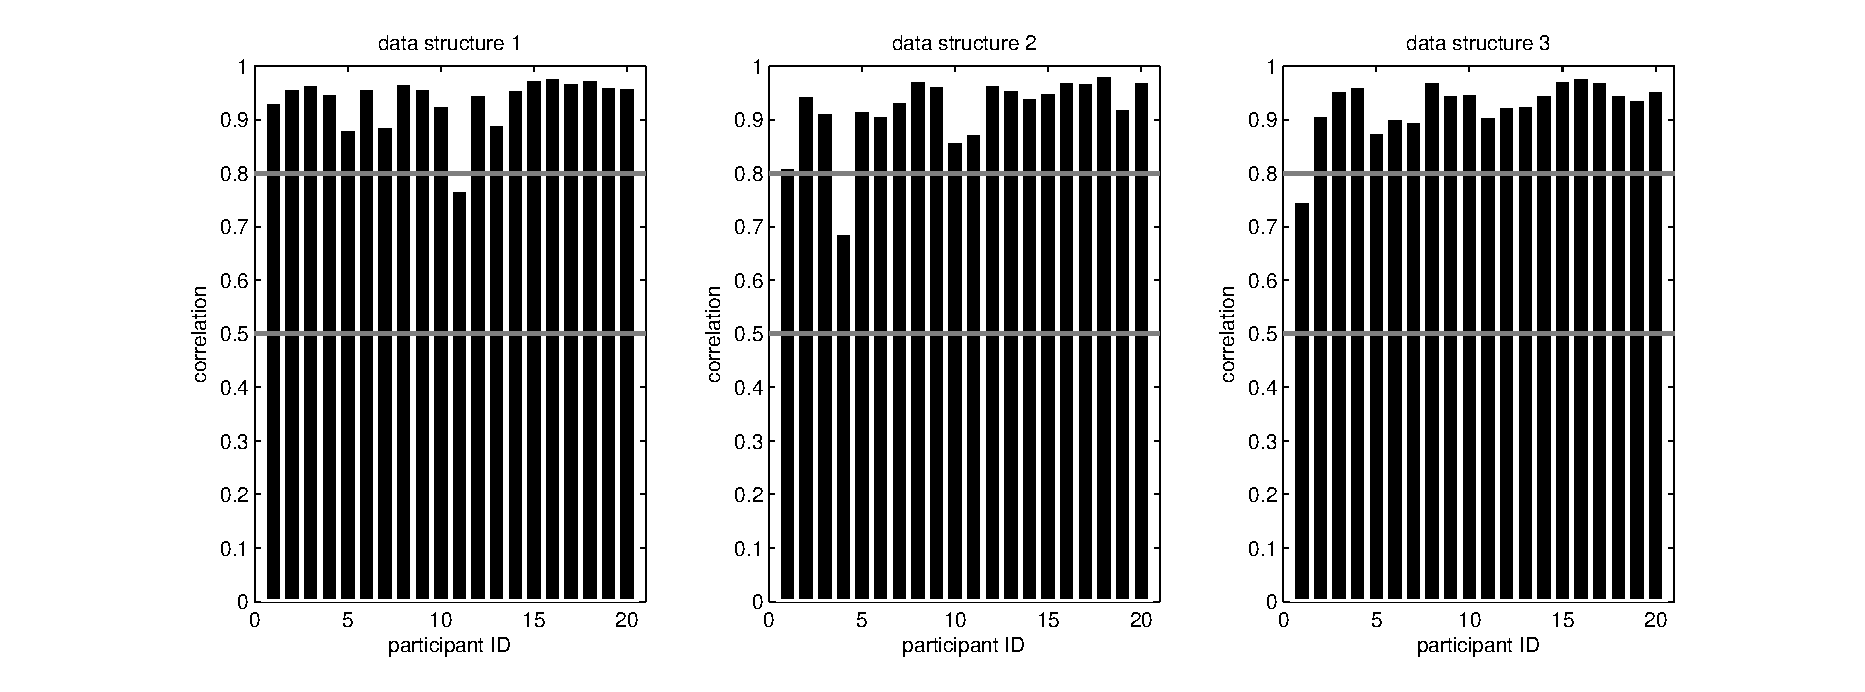
\epsfig{file=./figs/correlations2.eps,width=16cm}
\caption{Correlations between human data and model predictions in experiment 1, displayed for all 22 participants and all 3 data structures. All 60 correlations are significant at the .001 level, even after making degrees-of-freedom corrections for the two extra free parameters ($\theta$ and $\phi$). Grey bars plot the thresholds used to classify model performance as ``good'', ``moderate'' or ``poor''.}
\label{correl2}
\end{center}
\end{figure}


\subsection{Basic Results}

The analysis for experiment two proceeds in the same fashion as for experiment one. As before, we examine the 64 simple test cases to see whether the generalization gradients tighten due to sample size. If we translate the Likert scale responses to probability judgments in the obvious way (i.e., treating 1 as 0\%, 9 as 100\%, and interpolating linearly for all other values) then what we observe in the data corresponds to an average decrease in generalization probabilities of 3.0\%. Once again, this is significant ($t_{1299}=-6.5$, $p<.001$) but weak effect, of a similar magnitude to the 2.3\% decrease found in experiment one.


\subsection{Model-Based Analyses}

As with experiment one, we found the best-fitting values of $\theta$ and $\phi$ for each participant and each scenario. The correlations between model predictions and human responses were somewhat higher in experiment two. As shown in Figure~\ref{correl2}, all 60 correlations were significant, with a median of .90 and interquartile range of [.83, .94]. Overall, the model performance is at least moderately good in all cases, and is usually very good.

The main difference between experiment one and experiment two is that the cover story, data structure and the sampling scheme implied by the cover story were all varied independently. After checking that (as expected) there were no effects of the cover story itself (i.e., no differences between bobo fruits, walking birds and pikki-pikki leaves) and no interaction effects, we ran a $3 \times 2$ ANOVA with main effect terms for data structure and sampling scheme (weak vs strong) implied by the cover story, using the best-fitting value of $\theta$ as the dependent variable. The results suggest that the data structure influenced the choice of $\theta$ ($F_{2,52}=2.98, p = .06$), but that people did not make adjustments to $\theta$ as a result of the different sampling schemes implied by the cover story  ($F_{1,52}=0.004, p = .95$).

\begin{figure}[t]
\begin{center}
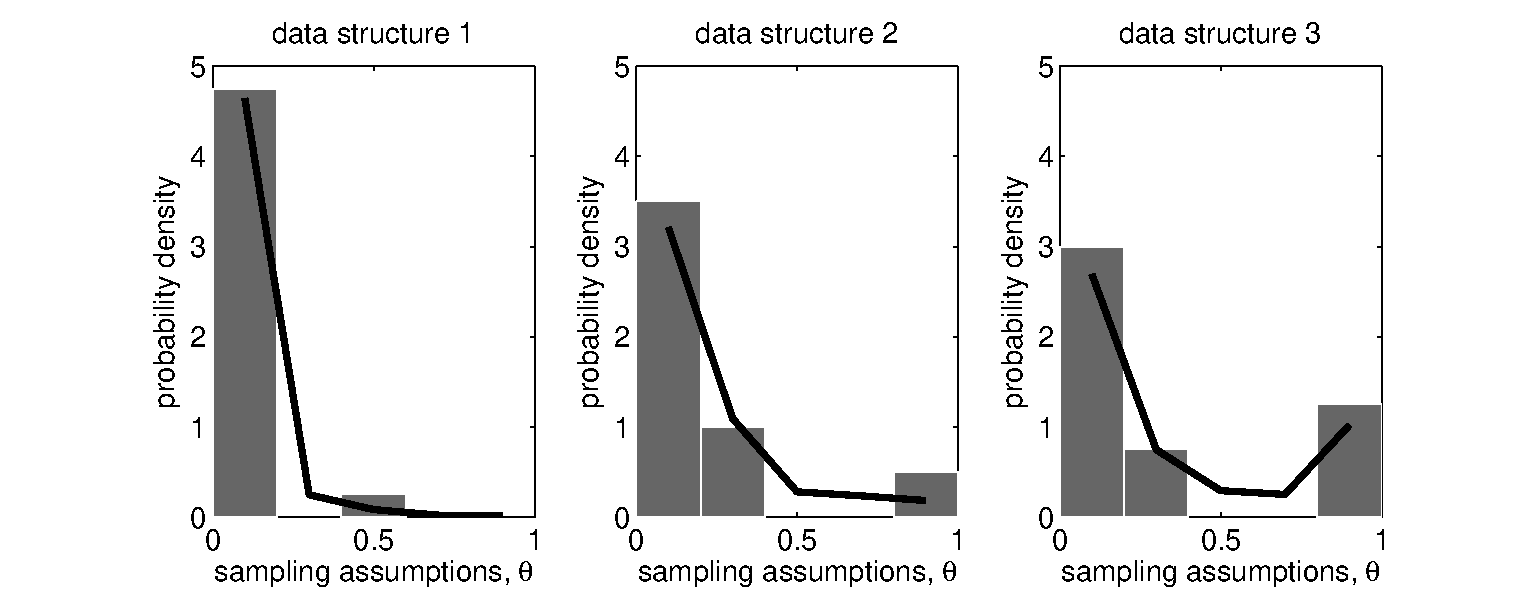
\epsfig{file=./figs/marginalposteriors_expt2.eps,width=15cm}
\caption{Distributions over $\theta$ observed in experiment 2. Each panel plots the distribution of best estimates (grey histograms) across the 20 participants, with each panel corresponding to one of the three data structures. (Black lines plot essentially the same analysis, but using the full posterior distributions over $\theta$ rather than just the best estimate for each participant).}
\label{margpost2}
\end{center}
\end{figure}

\subsection{Discussion}

Overall, the results from experiment two replicate those from experiment one, and suggest that the differences in $\theta$ across conditions are largely due to the data structure and not to an implicit instruction buried in the cover story. Consistent with our original intuition, the cover stories in these experiments are too ``generic'' to induce strong differences in people's sampling assumptions.

A question that these results raise is why there was no effect of cover story, especially in light of the results of \citeA{Xu2007b}. One possibility might be that the participants simply did not read the cover story closely, and hence did not take the implied sampling scheme into account. This seems rather unlikely, since the participants were explicitly told to pay close attention to the story. This is no guarantee that they did, but most participants did spend some time reading the stories. More plausibly, the manipulation may simply have been too subtle: people may not have given a great deal of thought to the implied sampling assumptions, and made no accommodation of them as a result. This suggests that a more overt manipulation of actual sampling procedures (such as the one used by \citeA{Xu2007b}) is likely to have an effect, but subtle differences in cover story may not. In the meantime, it seems that it is the data structure that is the origin of the effect. One possible reason for this might be that people are learning about the sampling model itself as the experiment progresses, and that the 1:3:5 structure induces a different amount of learning to the 3:5:10 scenarios. Future research might address this possibility.








\section{The Sampling Assumptions of Individuals}



Between the two experiments there are a total of 126 posterior distributions over $\theta$ (42 participants $\times$ 3 scenarios each). In the analyses presented up to this point we have attempted to summarize these individual distributions in terms of the marginal distributions in Figures~\ref{margpost1} and \ref{margpost2}. However, the aggregate distributions do not tell the whole story.

\begin{figure}[t]
\begin{center}
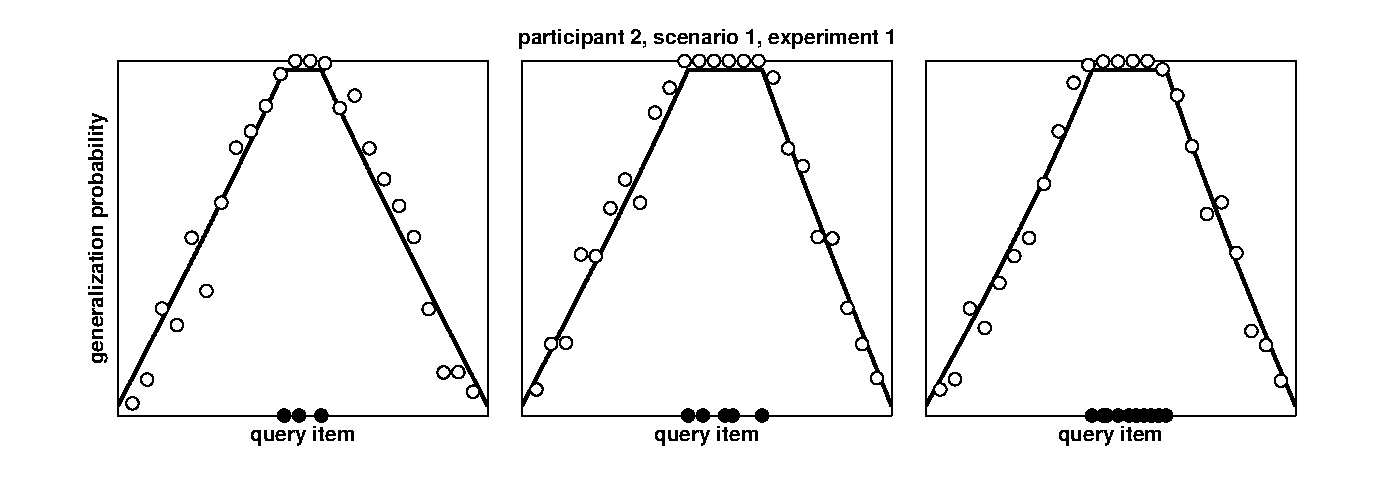
\epsfig{file=./figs/p2s1e1.eps, width=14cm}
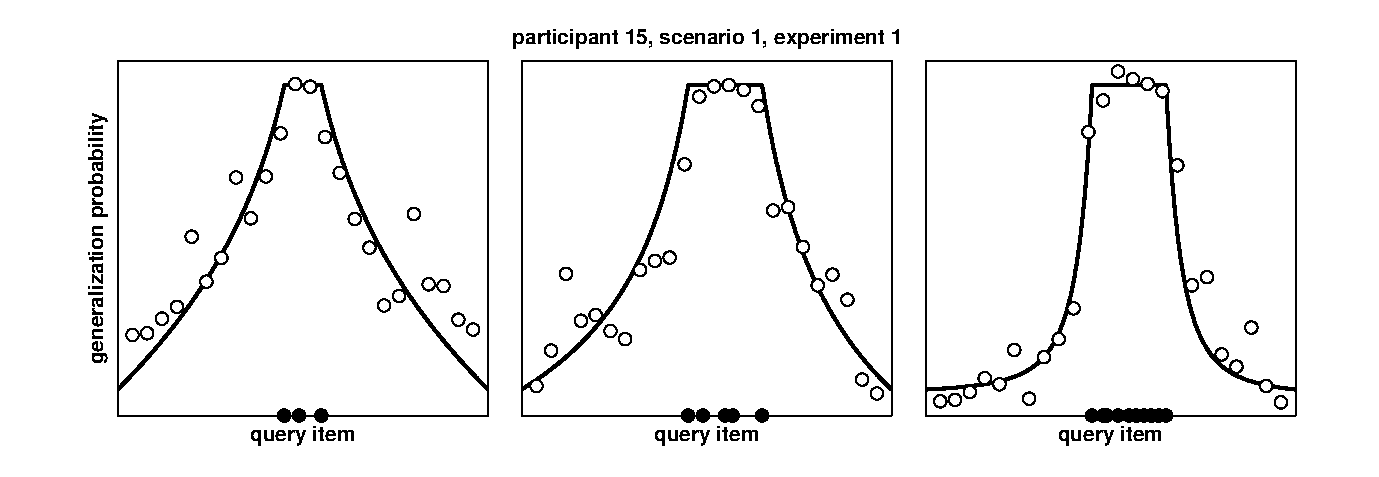
\epsfig{file=./figs/p15s1e1.eps, width=14cm}
\caption{A comparison between partipants 2 (top) and 15 (bottom) on scenario 1 (bacterial temperature), as the sample size is increased (from left to right). The solid black lines are the theoretical generalization gradients, and white circles denote the actual responses given. Black circles show the observations given to the participants. Parameter estimates are $\theta = .02$ and $\phi = 1.03$ for participant 2, and $\theta = .47$ and $\phi = 1.71$ for participant 15.}
\label{comp1}
\end{center}
\end{figure}

\begin{figure}[t]
\begin{center}
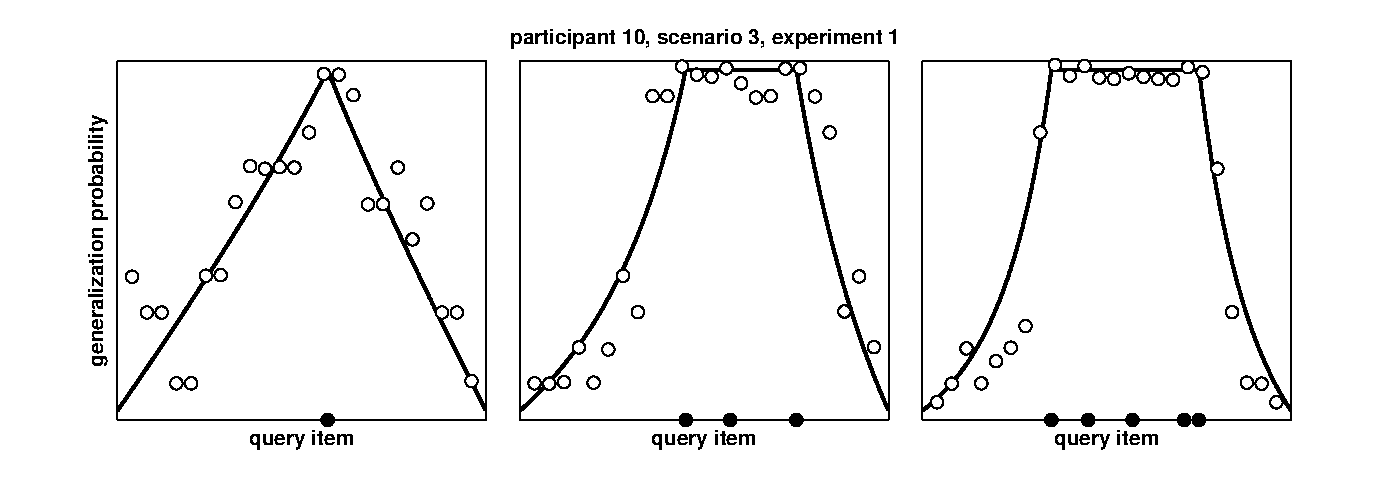
\epsfig{file=./figs/p10s3e1.eps, width=14cm}
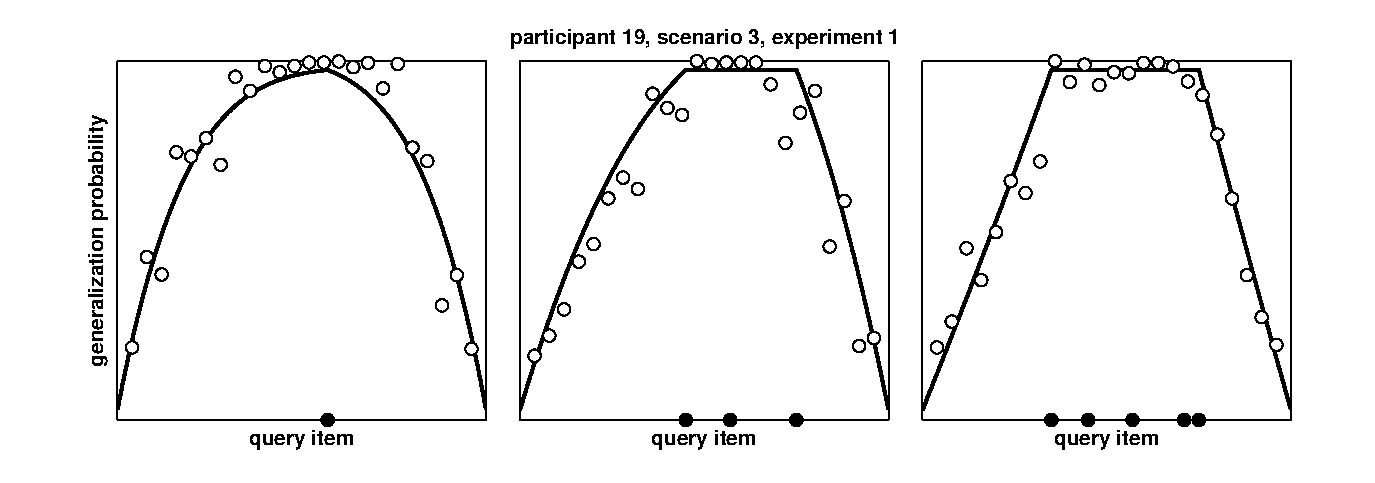
\epsfig{file=./figs/p19s3e1.eps, width=14cm}
\caption{Comparing two people with different priors and the same likelihood. Data are from participants 10 (top) and 19 (bottom), for the foraging scenario. For both participants the most likely sampling model was a purely strong account, with $\theta = 1$, but the best fitting value of $\phi$ differed. Participant 10 uses a prior that has very little by way of bias ($\phi = 1.79$) whereas participant 19 has a quite strong prior bias to expect the concept to have fairly broad extension ($\phi = 5.77$). The key thing to note is that the participants have very different generalization profiles when only a single datum is observed (left panels), but these differences begin to disappear as more data arrive (right panels).}
\label{comp2}
\end{center}
\end{figure}




Firstly, a focus on the aggregate distributions and goodness of fit statistics tends to obscure the actual behavior of people and the model. For instance, consider the comparison between the data from participants 2 and 15 in the bacterial temperatures scenario from experiment 1, shown in Figure~\ref{comp1}. In the first panel, the generalization gradients are quite similar, because the differences in priors ($\phi = 1.03$ and $\phi = 1.71$ respectively) are almost perfectly balanced by the differences in sampling assumptions ($\theta = .02$ and $\theta = .47$) when the learner has seen only three observations. However, as more data are observed, the two people diverge in their predictions, because the differences in the likelihood functions comes to dominate their beliefs. Analogous examples can be found in experiment 2.

The opposite effect can be seen by comparing participants 10 and 19 on scenario 3 in experiment 1. These two people have different priors ($\phi =1.79$ and $\phi = 5.77$ respectively) but the same likelihood (best fitting value is $\theta =1$ in both cases). When only a single datum is observed (left panels) these participants behave in quite different ways, but these differences begin to disappear as more data arrive (right panels). As is generally the case with Bayesian models, the data ``swamp'' the prior. That is, in the previous comparison (Figure~\ref{comp1}), participants made different assumptions about sampling, and so grew more dissimilar as the sample size increased. However, in this second comparison (Figure~\ref{comp2}), participants agree about how data are produced: as a consequence, their prior differences are erased as the sample size increases from left to right.

The second thing that is missing from the earlier analyses is a detailed examination of the posterior distributions over $\theta$ for each participant. In analyses to this point we have focused on the best fitting values of $\theta$, giving little consideration to the full posterior distribution. Nevertheless, for each participant and each scenario we have 72 judgments available, so the analysis is worth doing. We used standard Markov chain Monte Carlo techniques \cite<MCMC; >{Gilks1996} to estimate a complete posterior distribution over $\theta$ for every participant and every scenario (assuming a uniform prior). Specifically, we employ a Metropolis sampler with Gaussian proposal distribution, with burn in of 1000 iterations, and the distributions are estimated using 5000 samples drawn at a lag of 10 iterations between successive samples.

For experiment one, Figure~\ref{indiv1} plots each of the 66 posterior distributions over $\theta$ separately. As is clear from inspection, the apparent bimodality involved in the foraging scenario is an artifact of aggregating over participants. All of the individual distributions over $\theta$ are unimodal, but they are centered on different values. For both the bacterial and soil scenarios, most people either adopted a weak sampling model, or else used a mixed sampling model centered on a fairly modest value of $\theta$. For the foraging scenario, however, larger values of $\theta$ dominate, with only a few participants adopting weak sampling assumptions. The corresponding plots for experiment two are shown in Figure~\ref{indiv2}, and shows a similar pattern.




\begin{figure}
\begin{center}
\begin{tabular}{c}
(a) bacterial temperature scenario \\
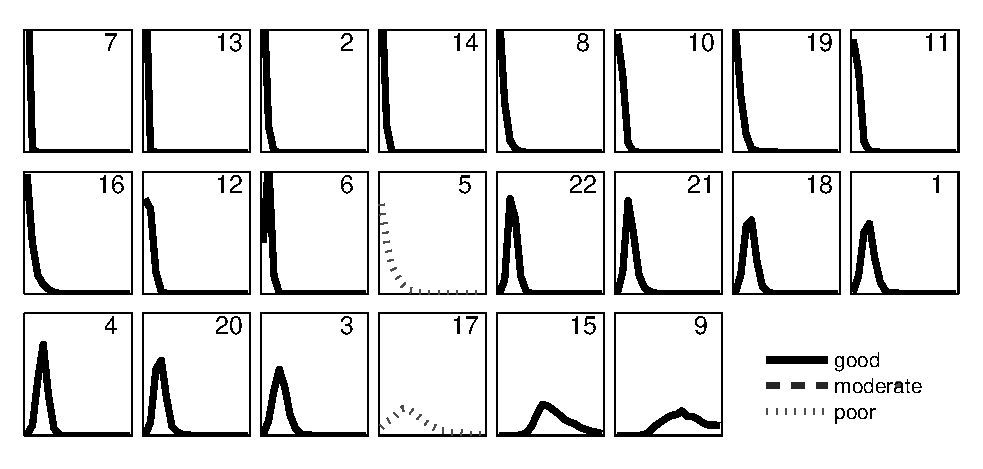
\epsfig{file=./figs/indivsubjexpt1cond1.eps,width=12cm} \\
(b) soil pH scenario \\
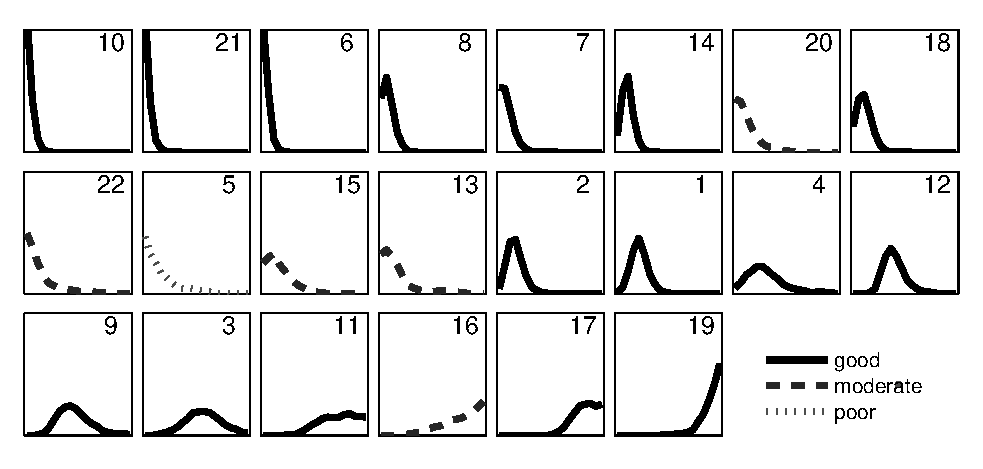
\epsfig{file=./figs/indivsubjexpt1cond2.eps,width=12cm} \\
(c) foraging hours scenario \\
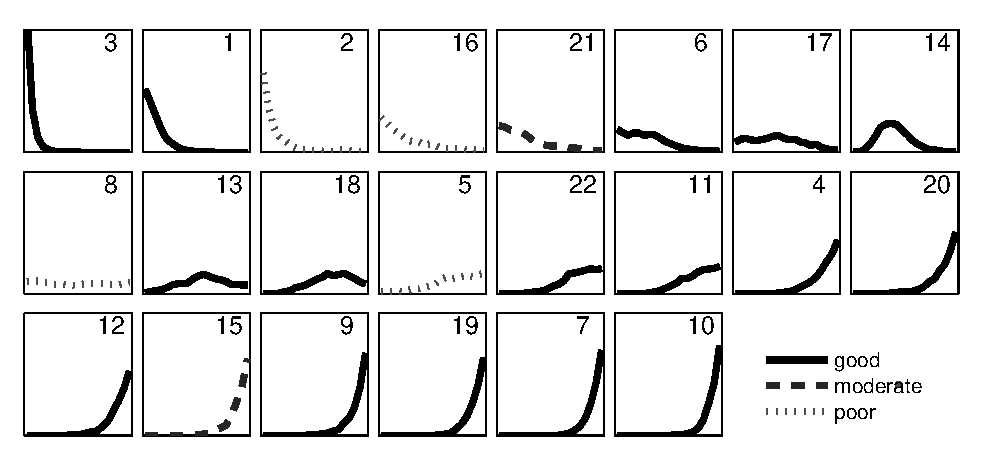
\epsfig{file=./figs/indivsubjexpt1cond3.eps,width=12cm}
\end{tabular}
\caption{Posterior distributions over $\theta$ for each participant, for all three scenarios in experiment 1. In these plots, we treated the model fit as ``good'' if the model correlated above 0.8 with the raw data, ``moderate'' if the correlation was between 0.5 and 0.8, and ``poor'' if the correlation fell below 0.5. All plots are on the same scale, with $\theta$ ranging from 0 to 1 on the horizontal axis and the probability density ranging from 0 to 12 on the vertical axis.}
\label{indiv1}
\end{center}
\end{figure}

\begin{figure}
\begin{center}
\begin{tabular}{c}
(a) data structure 1 \\
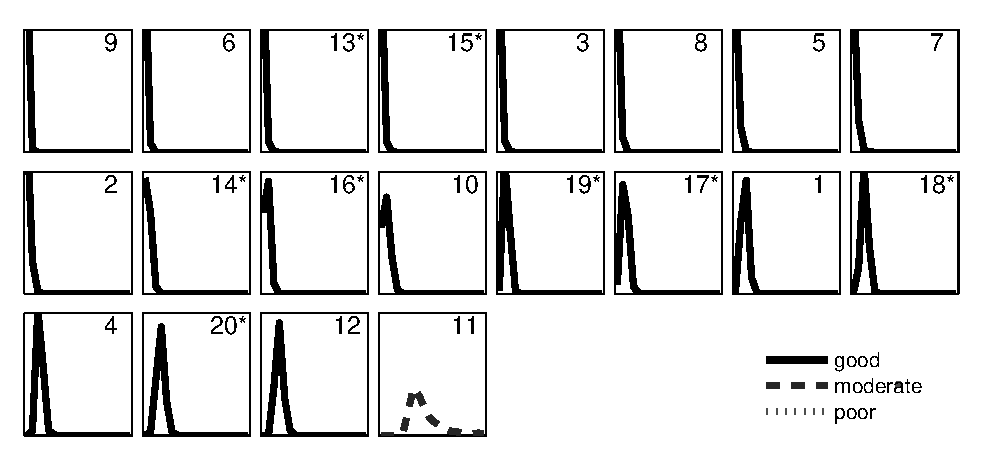
\epsfig{file=./figs/indivsubjexpt2cond1.eps,width=12cm} \\
(b) data structure 2 \\
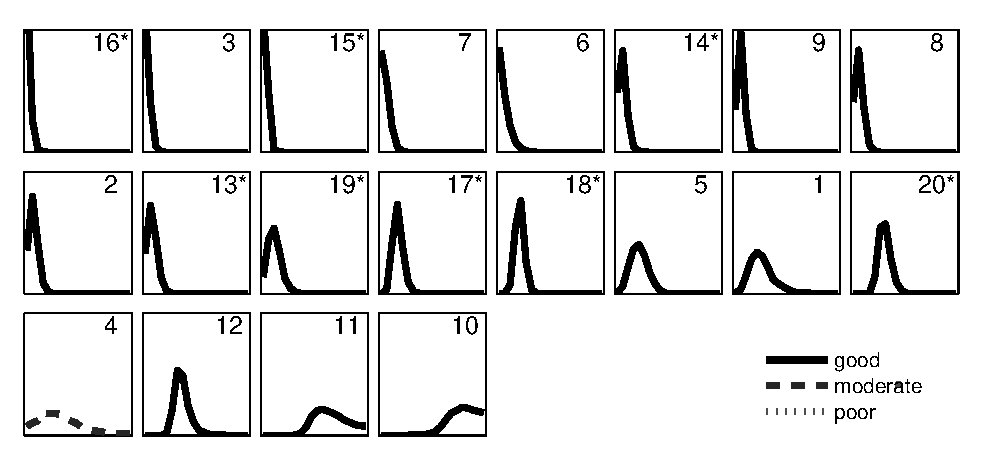
\epsfig{file=./figs/indivsubjexpt2cond2.eps,width=12cm} \\
(c) data structure 3 \\
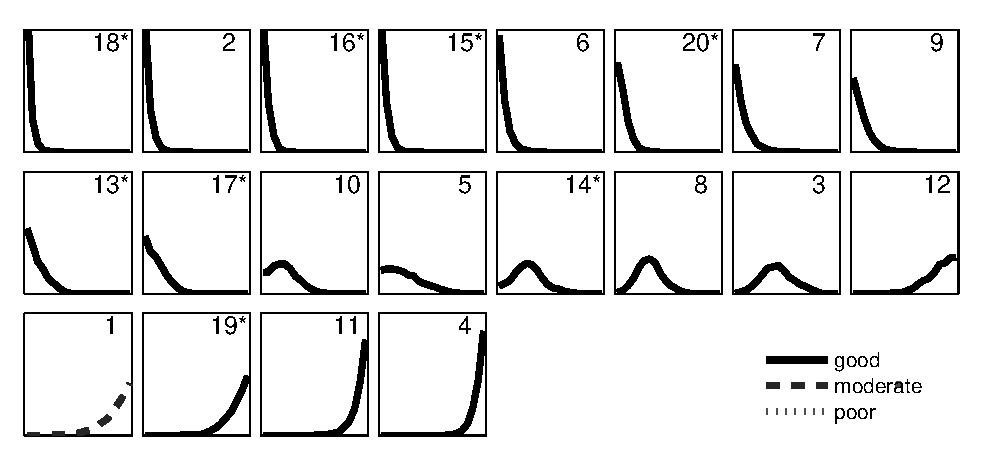
\epsfig{file=./figs/indivsubjexpt2cond3.eps,width=12cm}
\end{tabular}
\caption{Posterior distributions over $\theta$ for each participant, for all three data structures in experiment 2. Starred cases correspond to participants who saw the cover story in the strong sampling form. In these plots, we treated the model fit as ``good'' if the model correlated above 0.8 with the raw data, ``moderate'' if the correlation was between 0.5 and 0.8, and ``poor'' if the correlation fell below 0.5. All plots are on the same scale, with $\theta$ ranging from 0 to 1 on the horizontal axis and the probability density ranging from 0 to 12 on the vertical axis.}
\label{indiv2}
\end{center}
\end{figure}




\section{General Discussion}

The tendency to observe modest but non-zero values of $\theta$ in the experiments is strikingly similar to the phenomenon of conservatism in decision-making: people's belief revision tends to be slower than the rate predicted by simple Bayesian models  \cite<e.g.,>{Phillips1966}. In the experiments reported here, there is a sense in which $\theta=1$ is the ``correct'' sampling model to use, since the experimental design was such that all observed data points were constrained to lie inside the true consequential region $r$. Nevertheless, although some participants show clear evidence of having done so, most are at least a little conservative ($\theta <1$). Indeed, some participants do not adjust their generalization gradients at all ($\theta = 0$), appearing to be insensitive to the effects of increasing the sample size \cite<as per>{Tversky1974}.

Conservative sampling assumptions also help resolve an odd discrepancy between two different types of theory. Most category learning models \cite<e.g.>{Anderson1991a,Kruschke1992,Love2004} do not tighten the generalization gradients as the experiment progresses,\footnote{It is true that these models do adjust the generalization gradients in order to accommodate learned selective attention, the effect is generally to tighten generalization along one dimension at the expense of other dimensions. What is not generally part of the model is an overall tightening along all dimensions, as per strong sampling.} and are capable of fitting empirical data on the basis of this implicit weak sampling assumption. Our findings are more or less consistent with this: although a small number of people did display very strong tendencies to tighten their generalization gradients, most did not. The typical change of 2-3\% is small enough that it would probably not be noticed in a great many categorization experiments. This seems particularly likely in view of the fact that all of our problems were ``positive evidence only'' in design (in which strong sampling is the true model), whereas the majority of category learning experiments involve supervised classification designs (in which weak sampling is the true model). The conservative $\theta=.2$ value even in this case goes a long way toward explaining why strong sampling is not the typical assumption made when modeling category learning.

\begin{figure}[t]
\begin{center}
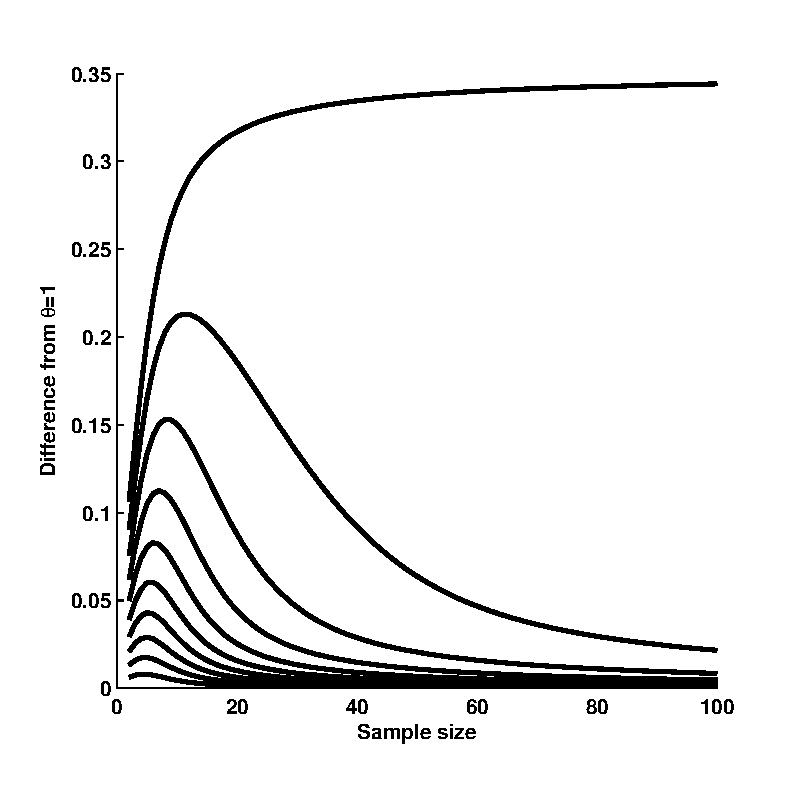
\epsfig{file=./figs/curvediscriminability.eps, width=9cm}
\caption{Distinguishability from the strong sampling case as sample size increases. Distinguishability is measured as the mean absolute difference in generalization probability across the entire range of possible query items [0,1], where training data always span the range [.3,.6]. The topmost curve plots the $\theta=0$ case, with the curves beneath increasing all the way to $\theta=1$ in increments of 0.1. Except for the pure weak sampling case, all sampling models eventually look indistinguishable from strong sampling as the sample size gets large.}
\label{asymptotics}
\end{center}
\end{figure}

In light of this result, the heavy reliance on strong sampling observed in other contexts \cite<e.g.,>{Tenenbaum2001,Xu2007} might seem unjustified. However, note that these models are typically concerned with {\it learnability} questions, often over developmental timeframes. In such cases, the critical problem facing the model is to ask how it is possible for the learner to acquire rich mental representations when exposed only to positive examples \cite{Muggleton1997}, and in order to do so, some variation of the strong sampling assumption is often implicitly adopted. For instance, in a language learning context, the amount of data strictly required to acquire abstract knowledge about syntax may be surprisingly small \cite{Perfors2006,Perforsunderreview}: the data presented to the model by \citeA{Perfors2006} corresponds only to a few hours of verbal input. In real life, of course, children require a great deal more data, presumably because they have other things to learn besides syntax, their raw data are messier than preprocessed corpus data, they have processing constraints that slow the learning, and so on. These factors should act to weaken the sampling model, but, as long as the resulting model is not strictly weak (i.e., as long as $\theta>0$), the learner should eventually acquire the knowledge in question. In fact, as Figure~\ref{asymptotics} illustrates for the spatial generalization problem we considered in this paper, as the sample size gets arbitrarily large, every sampling model {\it except} weak sampling eventually becomes indistinguishable, because they all converge on the true region. Thus, a learner who consistently employed a $\theta=.0001$ model would acquire knowledge in a fashion that is consistent with both the ``strong sampling'' pattern used in some models of language acquisition, and the ``weak sampling'' pattern often found in categorization experiments.



A number of other avenues for future work present themselves. Even within the context of simple spatial generalization problems, the assumption that the underlying hypothesis space consists solely of connected regions is probably too simple \cite{Tenenbaum2001a}. In particular, people may be willing to entertain the notion that the correct hypothesis consists of multiple regions \cite<see>[for a formalization of this idea]{Navarro2006}. To the extent that people believe that categories can cover multiple regions, the effects on the generalization gradients are likely to be twofold. Firstly, consistent with the general findings from our experiments, the generalization gradients over the {\it extrapolation} region (i.e., beyond the training data) should tighten more slowly than would be expected under the simpler model, because the learner remains open to the possibility that there exists some additional region of the stimulus space for which the hypothesis is true, about which they have yet to uncover any information. Secondly, the generalization gradients will not remain flat inside the {\it interpolation} region, because the learner must entertain the hypothesis that the training data that he or she has seen actually come from multiple regions. In fact, Figure~\ref{sampleraw} shows evidence of this effect. Participant 14 (dark lines) decreases the generalization probability in the gaps between training examples, whereas participant 2 (lighter lines) does not. More generally, if we examine the interpolation judgments across experiment one generally there is a weak correlation (Spearman's $\rho=-.16$, $p\approx 10^{-5}$) between the generalization probability and the distance from the nearest training exemplar to the query items. This is both consistent with standard exemplar models, as well as with Bayesian generalization models that allow multiple regions. However, since the experimental designs used in this paper were not optimized for examining interpolative judgments (i.e., there is a strong ceiling effect in these data since most people gave generalization judgments very close to 1 for all interpolation questions) this remains an open question for future work.

The use of uniform distributions as a basic building block is fairly standard for models in which the learner's goal is to identify a ``consequential set'' \cite<e.g.>{Shepard1987,Tenenbaum2001,Sanjana2003,Navarro2006}, and helps avoid the circularity of explaining graded generalizations in terms of graded sampling distributions. However, it is important to recognize that it too is an over-simplification. One of the more interesting extensions that one might consider is the situation in which the learner has to determine {\it both} the extension of the consequential set itself (i.e., which things are admissable members of the category) as well as the distribution over those entities (i.e., which things are more typical members of the category). Along similar lines, we have considered only those situations in which the learner observes positive and noise-free data from a single category. Natural extensions to the work would look at how sampling assumptions operate in other experimental designs, and in the presence of labeling noise.  In the meantime, however, it seems reasonable to conclude that individual participant's inductive generalizations are in close agreement with the predictions of the Bayesian theory, but vary considerably in terms of the default assumptions about how data were generated.


%\bibliography{djn}


\begin{thebibliography}{}

\bibitem[\protect\citeauthoryear{%
Anderson%
}{%
Anderson%
}{%
{\protect\APACyear{1991}}%
}]{%
Anderson1991a}%
\APACinsertmetastar{%
Anderson1991a}%
Anderson, J\BPBI R.%
%
\unskip\
\newblock
\APACrefYearMonthDay{1991}{}{}.
\newblock
\BBOQ{}\APACrefatitle{The adaptive nature of human categorization}{The adaptive
  nature of human categorization}.\BBCQ{}
\newblock
\APACjournalVolNumPages{Psychological Review}{98}{3}{409--429}.
\PrintBackRefs{\CurrentBib}

\bibitem[\protect\citeauthoryear{%
Anderson%
\ \BBA{} Milson%
}{%
Anderson%
\ \BBA{} Milson%
}{%
{\protect\APACyear{1989}}%
}]{%
Anderson1989}%
\APACinsertmetastar{%
Anderson1989}%
Anderson, J\BPBI R.%
\BCBT{}\ \BBA{} Milson, R.%
%
\unskip\
\newblock
\APACrefYearMonthDay{1989}{}{}.
\newblock
\BBOQ{}\APACrefatitle{Human memory: {A}n adaptive perspective}{Human memory:
  {A}n adaptive perspective}.\BBCQ{}
\newblock
\APACjournalVolNumPages{Psychological Review}{96}{}{703-719}.
\PrintBackRefs{\CurrentBib}

\bibitem[\protect\citeauthoryear{%
Anderson%
\ \BBA{} Schooler%
}{%
Anderson%
\ \BBA{} Schooler%
}{%
{\protect\APACyear{1991}}%
}]{%
Anderson1991}%
\APACinsertmetastar{%
Anderson1991}%
Anderson, J\BPBI R.%
\BCBT{}\ \BBA{} Schooler, L\BPBI J.%
%
\unskip\
\newblock
\APACrefYearMonthDay{1991}{}{}.
\newblock
\BBOQ{}\APACrefatitle{Reflections of the environment in memory}{Reflections of
  the environment in memory}.\BBCQ{}
\newblock
\APACjournalVolNumPages{Psychological Science}{2}{}{396-408}.
\PrintBackRefs{\CurrentBib}

\bibitem[\protect\citeauthoryear{%
Ennis%
}{%
Ennis%
}{%
{\protect\APACyear{1988}}%
}]{%
Ennis1988}%
\APACinsertmetastar{%
Ennis1988}%
Ennis, D\BPBI M.%
%
\unskip\
\newblock
\APACrefYearMonthDay{1988}{}{}.
\newblock
\BBOQ{}\APACrefatitle{Confusable and discriminable stimuli: {C}omment on
  {N}osofsky (1986) and {S}hepard (1986)}{Confusable and discriminable stimuli:
  {C}omment on {N}osofsky (1986) and {S}hepard (1986)}.\BBCQ{}
\newblock
\APACjournalVolNumPages{Journal of Experimental Psychology:
  General}{117}{}{408-411}.
\PrintBackRefs{\CurrentBib}

\bibitem[\protect\citeauthoryear{%
Estes%
}{%
Estes%
}{%
{\protect\APACyear{1956}}%
}]{%
Estes1956}%
\APACinsertmetastar{%
Estes1956}%
Estes, W\BPBI K.%
%
\unskip\
\newblock
\APACrefYearMonthDay{1956}{}{}.
\newblock
\BBOQ{}\APACrefatitle{The problem of inference from curves based on group
  data}{The problem of inference from curves based on group data}.\BBCQ{}
\newblock
\APACjournalVolNumPages{Psychological Bulletin}{53}{}{134-140.}
\PrintBackRefs{\CurrentBib}

\bibitem[\protect\citeauthoryear{%
Gigerenzer%
\ \BBA{} Brighton%
}{%
Gigerenzer%
\ \BBA{} Brighton%
}{%
{\protect\APACyear{2009}}%
}]{%
Gigerenzer2009}%
\APACinsertmetastar{%
Gigerenzer2009}%
Gigerenzer, G.%
\BCBT{}\ \BBA{} Brighton, H.%
%
\unskip\
\newblock
\APACrefYearMonthDay{2009}{}{}.
\newblock
\BBOQ{}\APACrefatitle{Homo Heuristicus: Why Biased Minds Make Better
  Inferences}{Homo heuristicus: Why biased minds make better
  inferences}.\BBCQ{}
\newblock
\APACjournalVolNumPages{Topics in Cognitive Science}{1}{}{107Ð143}.
\PrintBackRefs{\CurrentBib}

\bibitem[\protect\citeauthoryear{%
Gigerenzer%
\ \BBA{} Goldstein%
}{%
Gigerenzer%
\ \BBA{} Goldstein%
}{%
{\protect\APACyear{1996}}%
}]{%
Gigerenzer1996}%
\APACinsertmetastar{%
Gigerenzer1996}%
Gigerenzer, G.%
\BCBT{}\ \BBA{} Goldstein, D\BPBI G.%
%
\unskip\
\newblock
\APACrefYearMonthDay{1996}{}{}.
\newblock
\BBOQ{}\APACrefatitle{Reasoning the fast and frugal way: Models of bounded
  rationality}{Reasoning the fast and frugal way: Models of bounded
  rationality}.\BBCQ{}
\newblock
\APACjournalVolNumPages{Psychological Review}{103}{}{650-669}.
\PrintBackRefs{\CurrentBib}

\bibitem[\protect\citeauthoryear{%
Gilks%
, Richardson%
\BCBL{}\ \BBA{} Spiegelhalter%
}{%
Gilks%
\ \protect\BOthers{.}}{%
{\protect\APACyear{1996}}%
}]{%
Gilks1996}%
\APACinsertmetastar{%
Gilks1996}%
Gilks, W.%
, Richardson, S.%
\BCBL{}\ \BBA{} Spiegelhalter, D\BPBI J.%
\ (\BEDS).
\unskip\
\newblock
\APACrefYear{1996}.
\newblock
\APACrefbtitle{Markov Chain {M}onte {C}arlo in Practice}{Markov chain {M}onte
  {C}arlo in practice}.
\newblock
\APACaddressPublisher{Suffolk}{Chapman and Hall}.
\PrintBackRefs{\CurrentBib}

\bibitem[\protect\citeauthoryear{%
Gold%
}{%
Gold%
}{%
{\protect\APACyear{1967}}%
}]{%
Gold1967}%
\APACinsertmetastar{%
Gold1967}%
Gold, E\BPBI M.%
%
\unskip\
\newblock
\APACrefYearMonthDay{1967}{}{}.
\newblock
\BBOQ{}\APACrefatitle{Language identification in the limit}{Language
  identification in the limit}.\BBCQ{}
\newblock
\APACjournalVolNumPages{Information and Control}{10}{}{447-474}.
\PrintBackRefs{\CurrentBib}

\bibitem[\protect\citeauthoryear{%
Goldwater%
, Griffiths%
\BCBL{}\ \BBA{} Johnson%
}{%
Goldwater%
\ \protect\BOthers{.}}{%
{\protect\APACyear{2006}}%
}]{%
Goldwater2006}%
\APACinsertmetastar{%
Goldwater2006}%
Goldwater, S.%
, Griffiths, T\BPBI L.%
\BCBL{}\ \BBA{} Johnson, M.%
%
\unskip\
\newblock
\APACrefYearMonthDay{2006}{}{}.
\newblock
\BBOQ{}\APACrefatitle{Interpolating Between Types and Tokens by Estimating
  Power-Law Generators}{Interpolating between types and tokens by estimating
  power-law generators}.\BBCQ{}
\newblock
\BIn{} \APACrefbtitle{Advances in Neural Information Processing
  Systems}{Advances in neural information processing systems}\ (\BVOL~18).
\PrintBackRefs{\CurrentBib}

\bibitem[\protect\citeauthoryear{%
Goodman%
}{%
Goodman%
}{%
{\protect\APACyear{1955}}%
}]{%
Goodman1955}%
\APACinsertmetastar{%
Goodman1955}%
Goodman, N.%
%
\unskip\
\newblock
\APACrefYear{1955}.
\newblock
\APACrefbtitle{Fact, Fiction, and Forecast}{Fact, fiction, and forecast}.
\newblock
\APACaddressPublisher{Cambridge}{Harvard University Press}.
\PrintBackRefs{\CurrentBib}

\bibitem[\protect\citeauthoryear{%
Hastie%
, Tibshirani%
\BCBL{}\ \BBA{} Friedman%
}{%
Hastie%
\ \protect\BOthers{.}}{%
{\protect\APACyear{2001}}%
}]{%
Hastie2001}%
\APACinsertmetastar{%
Hastie2001}%
Hastie, T.%
, Tibshirani, R.%
\BCBL{}\ \BBA{} Friedman.%
%
\unskip\
\newblock
\APACrefYear{2001}.
\newblock
\APACrefbtitle{The Elements of Statistical Learning}{The elements of
  statistical learning}.
\newblock
\APACaddressPublisher{New York, NY}{Springer}.
\PrintBackRefs{\CurrentBib}

\bibitem[\protect\citeauthoryear{%
Hausser%
\ \BBA{} Strimmer%
}{%
Hausser%
\ \BBA{} Strimmer%
}{%
{\protect\APACyear{2009}}%
}]{%
Hausser2009}%
\APACinsertmetastar{%
Hausser2009}%
Hausser, J.%
\BCBT{}\ \BBA{} Strimmer, K.%
%
\unskip\
\newblock
\APACrefYearMonthDay{2009}{}{}.
\newblock
\BBOQ{}\APACrefatitle{Entropy Inference and the {J}ames-{S}tein Estimator, with
  Application to Nonlinear Gene Association Networks}{Entropy inference and the
  {J}ames-{S}tein estimator, with application to nonlinear gene association
  networks}.\BBCQ{}
\newblock
\APACjournalVolNumPages{Journal of Machine Learning Research}{10}{}{1469-1484}.
\PrintBackRefs{\CurrentBib}

\bibitem[\protect\citeauthoryear{%
Heit%
}{%
Heit%
}{%
{\protect\APACyear{1998}}%
}]{%
Heit1998}%
\APACinsertmetastar{%
Heit1998}%
Heit, E.%
%
\unskip\
\newblock
\APACrefYearMonthDay{1998}{}{}.
\newblock
\BBOQ{}\APACrefatitle{A {B}ayesian analysis of some forms of inductive
  reasoning}{A {B}ayesian analysis of some forms of inductive
  reasoning}.\BBCQ{}
\newblock
\BIn{} M.~Oaksford\ \BBA{} N.~Chater\ (\BEDS), \APACrefbtitle{Rational models
  of cognition}{Rational models of cognition}\ (\BPG~248-274).
\newblock
\APACaddressPublisher{Oxford}{Oxford University Press}.
\PrintBackRefs{\CurrentBib}

\bibitem[\protect\citeauthoryear{%
Hinton%
, McClelland%
\BCBL{}\ \BBA{} Rumelhart%
}{%
Hinton%
\ \protect\BOthers{.}}{%
{\protect\APACyear{1986}}%
}]{%
Hinton1986}%
\APACinsertmetastar{%
Hinton1986}%
Hinton, G\BPBI E.%
, McClelland, J\BPBI L.%
\BCBL{}\ \BBA{} Rumelhart, D\BPBI E.%
%
\unskip\
\newblock
\APACrefYearMonthDay{1986}{}{}.
\newblock
\BBOQ{}\APACrefatitle{Distributed representations}{Distributed
  representations}.\BBCQ{}
\newblock
\BIn{} D\BPBI E.~Rumelhart\ \BBA{} J\BPBI L.~McClelland\ (\BEDS),
  \APACrefbtitle{Parallel Distributed Processing: Explorations in the
  Microstructure of Cognition. Vol. 1: Foundations}{Parallel distributed
  processing: Explorations in the microstructure of cognition. vol. 1:
  Foundations}\ (\BPG~75-109).
\newblock
\APACaddressPublisher{Cambridge, MA}{MIT Press}.
\PrintBackRefs{\CurrentBib}

\bibitem[\protect\citeauthoryear{%
Huber%
}{%
Huber%
}{%
{\protect\APACyear{1981}}%
}]{%
Huber1981}%
\APACinsertmetastar{%
Huber1981}%
Huber, P\BPBI J.%
%
\unskip\
\newblock
\APACrefYear{1981}.
\newblock
\APACrefbtitle{Robust Statistics}{Robust statistics}.
\newblock
\APACaddressPublisher{New York}{Wiley}.
\PrintBackRefs{\CurrentBib}

\bibitem[\protect\citeauthoryear{%
James%
\ \BBA{} Stein%
}{%
James%
\ \BBA{} Stein%
}{%
{\protect\APACyear{1961}}%
}]{%
James1961}%
\APACinsertmetastar{%
James1961}%
James, W.%
\BCBT{}\ \BBA{} Stein, C.%
%
\unskip\
\newblock
\APACrefYearMonthDay{1961}{}{}.
\newblock
\BBOQ{}\APACrefatitle{Estimation with quadratic loss}{Estimation with quadratic
  loss}.\BBCQ{}
\newblock
\BIn{} \APACrefbtitle{Proceedings of the Fourth Berkeley Symposium on
  Mathematical Statistics and Probability, vol 1}{Proceedings of the fourth
  berkeley symposium on mathematical statistics and probability, vol 1}\
  (\BPG~361-379).
\PrintBackRefs{\CurrentBib}

\bibitem[\protect\citeauthoryear{%
Kemp%
\ \BBA{} Tenenbaum%
}{%
Kemp%
\ \BBA{} Tenenbaum%
}{%
{\protect\APACyear{2008}}%
}]{%
Kemp2008}%
\APACinsertmetastar{%
Kemp2008}%
Kemp, C.%
\BCBT{}\ \BBA{} Tenenbaum, J\BPBI B.%
%
\unskip\
\newblock
\APACrefYearMonthDay{2008}{}{}.
\newblock
\BBOQ{}\APACrefatitle{The discovery of structural form}{The discovery of
  structural form}.\BBCQ{}
\newblock
\APACjournalVolNumPages{Proceedings of the National Academy of
  Sciences}{105}{}{10687--10692}.
\PrintBackRefs{\CurrentBib}

\bibitem[\protect\citeauthoryear{%
Kemp%
\ \BBA{} Tenenbaum%
}{%
Kemp%
\ \BBA{} Tenenbaum%
}{%
{\protect\APACyear{2009}}%
}]{%
Kemp2009}%
\APACinsertmetastar{%
Kemp2009}%
Kemp, C.%
\BCBT{}\ \BBA{} Tenenbaum, J\BPBI B.%
%
\unskip\
\newblock
\APACrefYearMonthDay{2009}{}{}.
\newblock
\BBOQ{}\APACrefatitle{Structured statistical models of inductive
  reasoning}{Structured statistical models of inductive reasoning}.\BBCQ{}
\newblock
\APACjournalVolNumPages{Psychological Review}{116}{}{20-58}.
\PrintBackRefs{\CurrentBib}

\bibitem[\protect\citeauthoryear{%
Kruschke%
}{%
Kruschke%
}{%
{\protect\APACyear{1992}}%
}]{%
Kruschke1992}%
\APACinsertmetastar{%
Kruschke1992}%
Kruschke, J\BPBI K.%
%
\unskip\
\newblock
\APACrefYearMonthDay{1992}{}{}.
\newblock
\BBOQ{}\APACrefatitle{ALCOVE: An exemplar-based connectionist model of category
  learning}{Alcove: An exemplar-based connectionist model of category
  learning}.\BBCQ{}
\newblock
\APACjournalVolNumPages{Psychological Review}{99}{1}{22-44}.
\PrintBackRefs{\CurrentBib}

\bibitem[\protect\citeauthoryear{%
Lee%
, Chandrasena%
\BCBL{}\ \BBA{} Navarro%
}{%
Lee%
\ \protect\BOthers{.}}{%
{\protect\APACyear{2002}}%
}]{%
Lee2002c}%
\APACinsertmetastar{%
Lee2002c}%
Lee, M\BPBI D.%
, Chandrasena, L.%
\BCBL{}\ \BBA{} Navarro, D\BPBI J.%
%
\unskip\
\newblock
\APACrefYearMonthDay{2002}{}{}.
\newblock
\BBOQ{}\APACrefatitle{Using cognitive decision models to prioritize
  {E}-mails}{Using cognitive decision models to prioritize {E}-mails}.\BBCQ{}
\newblock
\BIn{} W\BPBI D.~Gray\ \BBA{} C\BPBI D.~Schunn\ (\BEDS),
  \APACrefbtitle{Proceedings of the 24th Annual Conference of the Cognitive
  Science Society (pp 478-483).}{Proceedings of the 24th annual conference of
  the cognitive science society (pp 478-483).}
\newblock
\APACaddressPublisher{Mahwah, NJ}{Lawrence Erlbaum}.
\PrintBackRefs{\CurrentBib}

\bibitem[\protect\citeauthoryear{%
Lee%
\ \BBA{} Webb%
}{%
Lee%
\ \BBA{} Webb%
}{%
{\protect\APACyear{2005}}%
}]{%
Lee2005b}%
\APACinsertmetastar{%
Lee2005b}%
Lee, M\BPBI D.%
\BCBT{}\ \BBA{} Webb, M\BPBI R.%
%
\unskip\
\newblock
\APACrefYearMonthDay{2005}{}{}.
\newblock
\BBOQ{}\APACrefatitle{Modeling individual differences in cognition}{Modeling
  individual differences in cognition}.\BBCQ{}
\newblock
\APACjournalVolNumPages{Psychonomic Bulletin \& Review}{12}{}{605-621}.
\PrintBackRefs{\CurrentBib}

\bibitem[\protect\citeauthoryear{%
Love%
, Medin%
\BCBL{}\ \BBA{} Gureckis%
}{%
Love%
\ \protect\BOthers{.}}{%
{\protect\APACyear{2004}}%
}]{%
Love2004}%
\APACinsertmetastar{%
Love2004}%
Love, B\BPBI C.%
, Medin, D\BPBI L.%
\BCBL{}\ \BBA{} Gureckis, T\BPBI M.%
%
\unskip\
\newblock
\APACrefYearMonthDay{2004}{}{}.
\newblock
\BBOQ{}\APACrefatitle{{SUSTAIN}: A network model of category
  learning}{{SUSTAIN}: A network model of category learning}.\BBCQ{}
\newblock
\APACjournalVolNumPages{Psychological Review}{11}{}{309-332}.
\PrintBackRefs{\CurrentBib}

\bibitem[\protect\citeauthoryear{%
Marr%
}{%
Marr%
}{%
{\protect\APACyear{1982}}%
}]{%
Marr1982}%
\APACinsertmetastar{%
Marr1982}%
Marr, D.%
%
\unskip\
\newblock
\APACrefYear{1982}.
\newblock
\APACrefbtitle{Vision}{Vision}.
\newblock
\APACaddressPublisher{San Francisco, CA}{W. H. Freeman}.
\PrintBackRefs{\CurrentBib}

\bibitem[\protect\citeauthoryear{%
Muggleton%
}{%
Muggleton%
}{%
{\protect\APACyear{1997}}%
}]{%
Muggleton1997}%
\APACinsertmetastar{%
Muggleton1997}%
Muggleton, S.%
%
\unskip\
\newblock
\APACrefYearMonthDay{1997}{}{}.
\newblock
\BBOQ{}\APACrefatitle{Learning from Positive Data}{Learning from positive
  data}.\BBCQ{}
\newblock
\BIn{} \APACrefbtitle{Selected Papers from the 6th International Workshop on
  Inductive Logic Programming}{Selected papers from the 6th international
  workshop on inductive logic programming}\ (\BPG~358-376).
\newblock
\APACaddressPublisher{}{Springer-Verlag}.
\PrintBackRefs{\CurrentBib}

\bibitem[\protect\citeauthoryear{%
I\BPBI J.~Myung%
}{%
I\BPBI J.~Myung%
}{%
{\protect\APACyear{2000}}%
}]{%
Myung2000b}%
\APACinsertmetastar{%
Myung2000b}%
Myung, I\BPBI J.%
%
\unskip\
\newblock
\APACrefYearMonthDay{2000}{}{}.
\newblock
\BBOQ{}\APACrefatitle{The importance of complexity in model selection}{The
  importance of complexity in model selection}.\BBCQ{}
\newblock
\APACjournalVolNumPages{Journal of Mathematical Psychology}{44}{}{190-204}.
\PrintBackRefs{\CurrentBib}

\bibitem[\protect\citeauthoryear{%
J\BPBI I.~Myung%
, Navarro%
\BCBL{}\ \BBA{} Pitt%
}{%
J\BPBI I.~Myung%
\ \protect\BOthers{.}}{%
{\protect\APACyear{2006}}%
}]{%
Myung2006}%
\APACinsertmetastar{%
Myung2006}%
Myung, J\BPBI I.%
, Navarro, D\BPBI J.%
\BCBL{}\ \BBA{} Pitt, M\BPBI A.%
%
\unskip\
\newblock
\APACrefYearMonthDay{2006}{}{}.
\newblock
\BBOQ{}\APACrefatitle{Model selection by {Normalized} {Maximum}
  {Likelihood}}{Model selection by {Normalized} {Maximum} {Likelihood}}.\BBCQ{}
\newblock
\APACjournalVolNumPages{Journal of Mathematical Psychology}{50}{}{167--179}.
\PrintBackRefs{\CurrentBib}

\bibitem[\protect\citeauthoryear{%
Navarro%
}{%
Navarro%
}{%
{\protect\APACyear{2006}}%
}]{%
Navarro2006}%
\APACinsertmetastar{%
Navarro2006}%
Navarro, D\BPBI J.%
%
\unskip\
\newblock
\APACrefYearMonthDay{2006}{}{}.
\newblock
\BBOQ{}\APACrefatitle{From natural kinds to complex categories}{From natural
  kinds to complex categories}.\BBCQ{}
\newblock
\BIn{} \APACrefbtitle{Proceedings of the 28th Annual Conference of the
  Cognitive Science Society}{Proceedings of the 28th annual conference of the
  cognitive science society}\ (\BPGS\ 621--626).
\newblock
\APACaddressPublisher{Mahwah, NJ}{Lawrence Erlbaum}.
\PrintBackRefs{\CurrentBib}

\bibitem[\protect\citeauthoryear{%
Navarro%
, Griffiths%
, Steyvers%
\BCBL{}\ \BBA{} Lee%
}{%
Navarro%
\ \protect\BOthers{.}}{%
{\protect\APACyear{2006}}%
}]{%
Navarro2006a}%
\APACinsertmetastar{%
Navarro2006a}%
Navarro, D\BPBI J.%
, Griffiths, T\BPBI L.%
, Steyvers, M.%
\BCBL{}\ \BBA{} Lee, M\BPBI D.%
%
\unskip\
\newblock
\APACrefYearMonthDay{2006}{}{}.
\newblock
\BBOQ{}\APACrefatitle{Modeling individual differences using {Dirichlet}
  processes}{Modeling individual differences using {Dirichlet}
  processes}.\BBCQ{}
\newblock
\APACjournalVolNumPages{Journal of Mathematical Psychology}{50}{}{101--122}.
\PrintBackRefs{\CurrentBib}

\bibitem[\protect\citeauthoryear{%
Navarro%
\ \BBA{} Perfors%
}{%
Navarro%
\ \BBA{} Perfors%
}{%
{\protect\APACyear{2010}}%
}]{%
Navarroinpress}%
\APACinsertmetastar{%
Navarroinpress}%
Navarro, D\BPBI J.%
\BCBT{}\ \BBA{} Perfors, A\BPBI F.%
%
\unskip\
\newblock
\APACrefYearMonthDay{2010}{}{}.
\newblock
\BBOQ{}\APACrefatitle{Similarity, feature discovery, and the size
  principle}{Similarity, feature discovery, and the size principle}.\BBCQ{}
\newblock
\APACjournalVolNumPages{Acta Psychologica}{133}{}{256-268}.
\PrintBackRefs{\CurrentBib}

\bibitem[\protect\citeauthoryear{%
Navon%
}{%
Navon%
}{%
{\protect\APACyear{1978}}%
}]{%
Navon1978}%
\APACinsertmetastar{%
Navon1978}%
Navon, D.%
%
\unskip\
\newblock
\APACrefYearMonthDay{1978}{}{}.
\newblock
\BBOQ{}\APACrefatitle{The importance of being conservative: {S}ome reflections
  on human {B}ayesian behavior}{The importance of being conservative: {S}ome
  reflections on human {B}ayesian behavior}.\BBCQ{}
\newblock
\APACjournalVolNumPages{British Journal of Mathematical and Statistical
  Psychology}{31}{}{33-48}.
\PrintBackRefs{\CurrentBib}

\bibitem[\protect\citeauthoryear{%
Nosofsky%
}{%
Nosofsky%
}{%
{\protect\APACyear{1984}}%
}]{%
Nosofsky1984}%
\APACinsertmetastar{%
Nosofsky1984}%
Nosofsky, R\BPBI M.%
%
\unskip\
\newblock
\APACrefYearMonthDay{1984}{}{}.
\newblock
\BBOQ{}\APACrefatitle{Choice, similarity and the context theory of
  classification}{Choice, similarity and the context theory of
  classification}.\BBCQ{}
\newblock
\APACjournalVolNumPages{Journal of Experimental Psychology: Learning, Memory,
  and Cognition}{10}{1}{104-114}.
\PrintBackRefs{\CurrentBib}

\bibitem[\protect\citeauthoryear{%
Osherson%
, Smith%
, Wilkie%
, Lopez%
\BCBL{}\ \BBA{} Shafir%
}{%
Osherson%
\ \protect\BOthers{.}}{%
{\protect\APACyear{1990}}%
}]{%
Osherson1990}%
\APACinsertmetastar{%
Osherson1990}%
Osherson, D\BPBI N.%
, Smith, E\BPBI E.%
, Wilkie, O.%
, Lopez, A.%
\BCBL{}\ \BBA{} Shafir, E.%
%
\unskip\
\newblock
\APACrefYearMonthDay{1990}{}{}.
\newblock
\BBOQ{}\APACrefatitle{Category-based induction}{Category-based
  induction}.\BBCQ{}
\newblock
\APACjournalVolNumPages{Psychological Review}{97}{2}{185-200}.
\PrintBackRefs{\CurrentBib}

\bibitem[\protect\citeauthoryear{%
Pavlov%
}{%
Pavlov%
}{%
{\protect\APACyear{1927}}%
}]{%
Pavlov1927}%
\APACinsertmetastar{%
Pavlov1927}%
Pavlov, I\BPBI P.%
%
\unskip\
\newblock
\APACrefYear{1927}.
\newblock
\APACrefbtitle{Conditioned Reflexes}{Conditioned reflexes}.
\newblock
\APACaddressPublisher{London, UK}{Oxford University Press}.
\PrintBackRefs{\CurrentBib}

\bibitem[\protect\citeauthoryear{%
Perfors%
, Tenenbaum%
\BCBL{}\ \BBA{} Regier%
}{%
Perfors%
\ \protect\BOthers{.}}{%
{\protect\APACyear{2006}}%
}]{%
Perfors2006}%
\APACinsertmetastar{%
Perfors2006}%
Perfors, A\BPBI F.%
, Tenenbaum, J\BPBI B.%
\BCBL{}\ \BBA{} Regier, T.%
%
\unskip\
\newblock
\APACrefYearMonthDay{2006}{}{}.
\newblock
\BBOQ{}\APACrefatitle{Poverty of the stimulus? A rational approach}{Poverty of
  the stimulus? a rational approach}.\BBCQ{}
\newblock
\BIn{} \APACrefbtitle{Proceedings of the 28th Annual Conference of the
  Cognitive Science Society.}{Proceedings of the 28th annual conference of the
  cognitive science society.}
\newblock
\APACaddressPublisher{Mahwah, NJ}{Lawrence Erlbaum}.
\PrintBackRefs{\CurrentBib}

\bibitem[\protect\citeauthoryear{%
Perfors%
, Tenenbaum%
\BCBL{}\ \BBA{} Regier%
}{%
Perfors%
\ \protect\BOthers{.}}{%
{\protect\APACyear{under review}}%
}]{%
Perforsunderreview}%
\APACinsertmetastar{%
Perforsunderreview}%
Perfors, A\BPBI F.%
, Tenenbaum, J\BPBI B.%
\BCBL{}\ \BBA{} Regier, T.%
%
\unskip\
\newblock
\APACrefYearMonthDay{under review}{}{}.
\newblock
\BBOQ{}\APACrefatitle{The learnability of abstract syntactic principles}{The
  learnability of abstract syntactic principles}.\BBCQ{}
\newblock
\APACjournalVolNumPages{Manuscript under review}{}{}{}.
\PrintBackRefs{\CurrentBib}

\bibitem[\protect\citeauthoryear{%
Phillips%
\ \BBA{} Edwards%
}{%
Phillips%
\ \BBA{} Edwards%
}{%
{\protect\APACyear{1966}}%
}]{%
Phillips1966}%
\APACinsertmetastar{%
Phillips1966}%
Phillips, L\BPBI D.%
\BCBT{}\ \BBA{} Edwards, W.%
%
\unskip\
\newblock
\APACrefYearMonthDay{1966}{}{}.
\newblock
\BBOQ{}\APACrefatitle{Conservatism in a simple probability inference
  task}{Conservatism in a simple probability inference task}.\BBCQ{}
\newblock
\APACjournalVolNumPages{Journal of Experimental Psychology}{72}{}{346-357}.
\PrintBackRefs{\CurrentBib}

\bibitem[\protect\citeauthoryear{%
Pitt%
, Myung%
\BCBL{}\ \BBA{} Zhang%
}{%
Pitt%
\ \protect\BOthers{.}}{%
{\protect\APACyear{2002}}%
}]{%
Pitt2002}%
\APACinsertmetastar{%
Pitt2002}%
Pitt, M\BPBI A.%
, Myung, I\BPBI J.%
\BCBL{}\ \BBA{} Zhang, S.%
%
\unskip\
\newblock
\APACrefYearMonthDay{2002}{}{}.
\newblock
\BBOQ{}\APACrefatitle{Toward a method of selecting among computational models
  of cognition}{Toward a method of selecting among computational models of
  cognition}.\BBCQ{}
\newblock
\APACjournalVolNumPages{Psychological Review}{109}{3}{472-491}.
\PrintBackRefs{\CurrentBib}

\bibitem[\protect\citeauthoryear{%
Popper%
}{%
Popper%
}{%
{\protect\APACyear{1935/1990}}%
}]{%
Popper1935/1990}%
\APACinsertmetastar{%
Popper1935/1990}%
Popper, K\BPBI R.%
%
\unskip\
\newblock
\APACrefYear{1935/1990}.
\newblock
\APACrefbtitle{The Logic of Scientific Discovery}{The logic of scientific
  discovery}.
\newblock
\APACaddressPublisher{Boston, MA}{Unwin Hyman}.
\PrintBackRefs{\CurrentBib}

\bibitem[\protect\citeauthoryear{%
Ratcliff%
\ \BBA{} Tuerlinckx%
}{%
Ratcliff%
\ \BBA{} Tuerlinckx%
}{%
{\protect\APACyear{2002}}%
}]{%
Ratcliff2002}%
\APACinsertmetastar{%
Ratcliff2002}%
Ratcliff, R.%
\BCBT{}\ \BBA{} Tuerlinckx, F.%
%
\unskip\
\newblock
\APACrefYearMonthDay{2002}{}{}.
\newblock
\BBOQ{}\APACrefatitle{Estimating parameters of the diffusion model: Approaches
  to dealing with contaminant reaction times and parameter
  variability}{Estimating parameters of the diffusion model: Approaches to
  dealing with contaminant reaction times and parameter variability}.\BBCQ{}
\newblock
\APACjournalVolNumPages{Psychonomic Bulletin and Review}{9}{}{438-481}.
\PrintBackRefs{\CurrentBib}

\bibitem[\protect\citeauthoryear{%
Russell%
}{%
Russell%
}{%
{\protect\APACyear{1986}}%
}]{%
Russell1986}%
\APACinsertmetastar{%
Russell1986}%
Russell, S\BPBI J.%
%
\unskip\
\newblock
\APACrefYearMonthDay{1986}{}{}.
\newblock
\BBOQ{}\APACrefatitle{A quantitative analysis of analogy by similarity}{A
  quantitative analysis of analogy by similarity}.\BBCQ{}
\newblock
\BIn{} \APACrefbtitle{Proceedings of the National Conference on Artificial
  Intelligence}{Proceedings of the national conference on artificial
  intelligence}\ (\BPG~284-288).
\newblock
\APACaddressPublisher{Philadelphia, PA}{AAAI}.
\PrintBackRefs{\CurrentBib}

\bibitem[\protect\citeauthoryear{%
Sanjana%
\ \BBA{} Tenenbaum%
}{%
Sanjana%
\ \BBA{} Tenenbaum%
}{%
{\protect\APACyear{2003}}%
}]{%
Sanjana2003}%
\APACinsertmetastar{%
Sanjana2003}%
Sanjana, N\BPBI E.%
\BCBT{}\ \BBA{} Tenenbaum, J\BPBI B.%
%
\unskip\
\newblock
\APACrefYearMonthDay{2003}{}{}.
\newblock
\BBOQ{}\APACrefatitle{Bayesian models of inductive generalization}{Bayesian
  models of inductive generalization}.\BBCQ{}
\newblock
\BIn{} S.~Becker, S.~Thrun\BCBL{}\ \BBA{} K.~Obermayer\ (\BEDS),
  \APACrefbtitle{Advances in Neural Information Processing Systems}{Advances in
  neural information processing systems}\ (\BVOL~15, \BPG~51-58).
\newblock
\APACaddressPublisher{Cambridge, MA}{MIT Press}.
\PrintBackRefs{\CurrentBib}

\bibitem[\protect\citeauthoryear{%
Sch\"afer%
\ \BBA{} Strimmer%
}{%
Sch\"afer%
\ \BBA{} Strimmer%
}{%
{\protect\APACyear{2005}}%
}]{%
Schafer2005}%
\APACinsertmetastar{%
Schafer2005}%
Sch\"afer, J.%
\BCBT{}\ \BBA{} Strimmer, K.%
%
\unskip\
\newblock
\APACrefYearMonthDay{2005}{}{}.
\newblock
\BBOQ{}\APACrefatitle{A shrinkage approach to large-scale covariance matrix
  estimation and implications for functional genomics}{A shrinkage approach to
  large-scale covariance matrix estimation and implications for functional
  genomics}.\BBCQ{}
\newblock
\APACjournalVolNumPages{Statistical Applications in Genetics and Molecular
  Biology}{4}{}{}.
\PrintBackRefs{\CurrentBib}

\bibitem[\protect\citeauthoryear{%
Shepard%
}{%
Shepard%
}{%
{\protect\APACyear{1987}}%
}]{%
Shepard1987}%
\APACinsertmetastar{%
Shepard1987}%
Shepard, R\BPBI N.%
%
\unskip\
\newblock
\APACrefYearMonthDay{1987}{}{}.
\newblock
\BBOQ{}\APACrefatitle{Toward a universal law of generalization for
  psychological science}{Toward a universal law of generalization for
  psychological science}.\BBCQ{}
\newblock
\APACjournalVolNumPages{Science}{237}{}{1317-1323}.
\PrintBackRefs{\CurrentBib}

\bibitem[\protect\citeauthoryear{%
Sloman%
}{%
Sloman%
}{%
{\protect\APACyear{1993}}%
}]{%
Sloman1993}%
\APACinsertmetastar{%
Sloman1993}%
Sloman, S.%
%
\unskip\
\newblock
\APACrefYearMonthDay{1993}{}{}.
\newblock
\BBOQ{}\APACrefatitle{Feature-based induction}{Feature-based induction}.\BBCQ{}
\newblock
\APACjournalVolNumPages{Cognitive Psychology}{25}{}{231-280}.
\PrintBackRefs{\CurrentBib}

\bibitem[\protect\citeauthoryear{%
Solomonoff%
}{%
Solomonoff%
}{%
{\protect\APACyear{1964}}%
}]{%
Solomonoff1964}%
\APACinsertmetastar{%
Solomonoff1964}%
Solomonoff, R\BPBI J.%
%
\unskip\
\newblock
\APACrefYearMonthDay{1964}{}{}.
\newblock
\BBOQ{}\APACrefatitle{A formal theory of inductive inference. {P}art {I}}{A
  formal theory of inductive inference. {P}art {I}}.\BBCQ{}
\newblock
\APACjournalVolNumPages{Information and Control}{7}{}{1-22}.
\PrintBackRefs{\CurrentBib}

\bibitem[\protect\citeauthoryear{%
Stein%
}{%
Stein%
}{%
{\protect\APACyear{1956}}%
}]{%
Stein1956}%
\APACinsertmetastar{%
Stein1956}%
Stein, C.%
%
\unskip\
\newblock
\APACrefYearMonthDay{1956}{}{}.
\newblock
\BBOQ{}\APACrefatitle{Inadmissibility of the usual estimator for the mean of a
  multivariate distribution}{Inadmissibility of the usual estimator for the
  mean of a multivariate distribution}.\BBCQ{}
\newblock
\BIn{} \APACrefbtitle{Proceedings of the Third Berkeley Symposium on
  Mathematical Statistics and Probability, vol 1}{Proceedings of the third
  berkeley symposium on mathematical statistics and probability, vol 1}\
  (\BPG~197-206).
\PrintBackRefs{\CurrentBib}

\bibitem[\protect\citeauthoryear{%
Tenenbaum%
}{%
Tenenbaum%
}{%
{\protect\APACyear{1999}}%
}]{%
Tenenbaum1999}%
\APACinsertmetastar{%
Tenenbaum1999}%
Tenenbaum, J\BPBI B.%
%
\unskip\
\newblock
\APACrefYear{1999}.
\newblock
\APACrefbtitle{A {B}ayesian framework for concept learning}{A {B}ayesian
  framework for concept learning}.
\newblock
\BUPhD, Massachussets Institute of Technology, Cambridge, MA.
\PrintBackRefs{\CurrentBib}

\bibitem[\protect\citeauthoryear{%
Tenenbaum%
\ \BBA{} Griffiths%
}{%
Tenenbaum%
\ \BBA{} Griffiths%
}{%
{\protect\APACyear{2001}}%
{\protect\APACexlab{{\protect\BCnt{1}}}}}]{%
Tenenbaum2001}%
\APACinsertmetastar{%
Tenenbaum2001}%
Tenenbaum, J\BPBI B.%
\BCBT{}\ \BBA{} Griffiths, T\BPBI L.%
%
\unskip\
\newblock
\APACrefYearMonthDay{2001{\protect\BCnt{1}}}{}{}.
\newblock
\BBOQ{}\APACrefatitle{Generalization, similarity, and {B}ayesian
  inference}{Generalization, similarity, and {B}ayesian inference}.\BBCQ{}
\newblock
\APACjournalVolNumPages{Behavioral and Brain Sciences}{24}{}{629-641}.
\PrintBackRefs{\CurrentBib}

\bibitem[\protect\citeauthoryear{%
Tenenbaum%
\ \BBA{} Griffiths%
}{%
Tenenbaum%
\ \BBA{} Griffiths%
}{%
{\protect\APACyear{2001}}%
{\protect\APACexlab{{\protect\BCnt{2}}}}}]{%
Tenenbaum2001a}%
\APACinsertmetastar{%
Tenenbaum2001a}%
Tenenbaum, J\BPBI B.%
\BCBT{}\ \BBA{} Griffiths, T\BPBI L.%
%
\unskip\
\newblock
\APACrefYearMonthDay{2001{\protect\BCnt{2}}}{}{}.
\newblock
\BBOQ{}\APACrefatitle{Some specifics about generalization}{Some specifics about
  generalization}.\BBCQ{}
\newblock
\APACjournalVolNumPages{Behavioral and {Brain} {Sciences}}{24}{}{762-778}.
\PrintBackRefs{\CurrentBib}

\bibitem[\protect\citeauthoryear{%
Tversky%
}{%
Tversky%
}{%
{\protect\APACyear{1977}}%
}]{%
Tversky1977}%
\APACinsertmetastar{%
Tversky1977}%
Tversky, A.%
%
\unskip\
\newblock
\APACrefYearMonthDay{1977}{}{}.
\newblock
\BBOQ{}\APACrefatitle{Features of similarity}{Features of similarity}.\BBCQ{}
\newblock
\APACjournalVolNumPages{Psychological Review}{84}{4}{327-352}.
\PrintBackRefs{\CurrentBib}

\bibitem[\protect\citeauthoryear{%
Tversky%
\ \BBA{} Kahneman%
}{%
Tversky%
\ \BBA{} Kahneman%
}{%
{\protect\APACyear{1974}}%
}]{%
Tversky1974}%
\APACinsertmetastar{%
Tversky1974}%
Tversky, A.%
\BCBT{}\ \BBA{} Kahneman, D.%
%
\unskip\
\newblock
\APACrefYearMonthDay{1974}{}{}.
\newblock
\BBOQ{}\APACrefatitle{Judgment under uncertainty: heuristics and
  biases}{Judgment under uncertainty: heuristics and biases}.\BBCQ{}
\newblock
\APACjournalVolNumPages{Science}{185}{}{1124-1131}.
\PrintBackRefs{\CurrentBib}

\bibitem[\protect\citeauthoryear{%
Welsh%
\ \BBA{} Navarro%
}{%
Welsh%
\ \BBA{} Navarro%
}{%
{\protect\APACyear{2007}}%
}]{%
Welsh2007}%
\APACinsertmetastar{%
Welsh2007}%
Welsh, M\BPBI B.%
\BCBT{}\ \BBA{} Navarro, D\BPBI J.%
%
\unskip\
\newblock
\APACrefYear{2007}.
\newblock
\APACrefbtitle{Seeing is believing: {Priors}, trust and base rate
  neglect}{Seeing is believing: {Priors}, trust and base rate neglect}.
\newblock
\APACaddressPublisher{}{Proceedings of the 29th Annual Conference of the
  Cognitive Science Society}.
\PrintBackRefs{\CurrentBib}

\bibitem[\protect\citeauthoryear{%
Xu%
\ \BBA{} Tenenbaum%
}{%
Xu%
\ \BBA{} Tenenbaum%
}{%
{\protect\APACyear{2007}}%
{\protect\APACexlab{{\protect\BCnt{1}}}}}]{%
Xu2007b}%
\APACinsertmetastar{%
Xu2007b}%
Xu, F.%
\BCBT{}\ \BBA{} Tenenbaum, J\BPBI B.%
%
\unskip\
\newblock
\APACrefYearMonthDay{2007{\protect\BCnt{1}}}{}{}.
\newblock
\BBOQ{}\APACrefatitle{Sensitivity to sampling in {B}ayesian word
  learning}{Sensitivity to sampling in {B}ayesian word learning}.\BBCQ{}
\newblock
\APACjournalVolNumPages{Developmental Science}{10}{}{288-297}.
\PrintBackRefs{\CurrentBib}

\bibitem[\protect\citeauthoryear{%
Xu%
\ \BBA{} Tenenbaum%
}{%
Xu%
\ \BBA{} Tenenbaum%
}{%
{\protect\APACyear{2007}}%
{\protect\APACexlab{{\protect\BCnt{2}}}}}]{%
Xu2007}%
\APACinsertmetastar{%
Xu2007}%
Xu, F.%
\BCBT{}\ \BBA{} Tenenbaum, J\BPBI B.%
%
\unskip\
\newblock
\APACrefYearMonthDay{2007{\protect\BCnt{2}}}{}{}.
\newblock
\BBOQ{}\APACrefatitle{Word learning as {B}ayesian inference}{Word learning as
  {B}ayesian inference}.\BBCQ{}
\newblock
\APACjournalVolNumPages{Psychological Review}{114}{}{245-272}.
\PrintBackRefs{\CurrentBib}

\bibitem[\protect\citeauthoryear{%
Zeigenfuse%
\ \BBA{} Lee%
}{%
Zeigenfuse%
\ \BBA{} Lee%
}{%
{\protect\APACyear{2010}}%
}]{%
Zeigenfuseinpress}%
\APACinsertmetastar{%
Zeigenfuseinpress}%
Zeigenfuse, M\BPBI D.%
\BCBT{}\ \BBA{} Lee, M\BPBI D.%
%
\unskip\
\newblock
\APACrefYearMonthDay{2010}{}{}.
\newblock
\BBOQ{}\APACrefatitle{A general latent-assignment approach for modeling
  psychological contaminants}{A general latent-assignment approach for modeling
  psychological contaminants}.\BBCQ{}
\newblock
\APACjournalVolNumPages{Journal of Mathematical Psychology}{54}{}{354-362}.
\PrintBackRefs{\CurrentBib}

\end{thebibliography}
\clearpage

\appendix \section{}


\subsection{1. Analytic Expressions for the Generalization Model}
In this section, we derive exact expressions for the generalization probabilities referred to in the main text. We start by deriving the basic form for all such probabilities, then dealing with the weak sampling, strong sampling and mixed sampling cases in turn, under the assumption of uniform priors. We then extend this to the non-uniform case.

\subsubsection{Preliminaries} Let $x_i \in \mathcal{X}$ denote the location of the $i$th observed item, and let $\xn=(x_1, \ldots, x_n)$ denote the set of items known to belong to the same category. The learner assumes that every element of $\xn$ belongs to a single true region $\rt \in \mathcal{R}$. Since the tasks that we consider explicitly provide upper and lower bounds, we may assume without loss of generality that $\mathcal{X}=[0,1]$ and $\mathcal{R}$ consists of all closed intervals on $\mathcal{X}$. Given a novel stimulus with co-ordinate value $y$ are interested in $\p(y\in \rt \condon  \xn, \xn \in \rt)$, the probability that it is also in $\rt$.
\begin{eqnarray}
\p(y \in \rt \condon  \xn, \xn \in \rt) &=& \int_{\mathcal{R}} \p(y \in \rt \condon  \rt = r) \p(\rt = r \condon  \xn, \xn \in \rt) \ dr
\end{eqnarray}
where $r$ denotes one possibility as to the identity of the true region $\rt$, and the integration is taken over $\mathcal{R}$, the set of all such regions. Noting that $\p(y \in \rt \condon  \rt = r)$ equals 1 if $y$ falls inside $r$ and zero if it does not, we can expand the integral, and obtain:
\begin{eqnarray}
\p(y \in \rt \condon  \xn, \xn \in \rt) &=& \int_{\mathcal{R}} \p(y \in \rt \condon  \rt = r) \p(\rt = r \condon  \xn, \xn \in \rt) \ dr \nonumber \\
&=& \int_{\mathcal{R}_y}  \p(\rt = r \condon  \xn, \xn \in \rt) \ dr \nonumber \\
&=& \int_{\mathcal{R}_y} \frac{\p(\xn, \xn \in \rt \condon  \rt = r) \p(\rt=r)}{\p(\xn, \xn \in \rt)}  \ dr \nonumber \\
&=& \frac{\int_{\mathcal{R}_y} \p(\xn, \xn \in \rt\condon  \rt =r ) \p(\rt=r) \ dr}{\int_{\mathcal{R}}\p(\xn, \xn \in \rt \condon  \rt=r) \p(\rt=r) \ dr}
\end{eqnarray}
where $\mathcal{R}_y \subset \mathcal{R}$ denotes the set of possible regions that include $y$.
We initially assume a uniform prior over regions, $\p(\rt=r) \propto 1$, and hence this expression simplifies to
\begin{eqnarray}
\p(y \in \rt \condon  \xn, \xn \in \rt)
&=& \frac{\int_{\mathcal{R}_y} \p(\xn, \xn \in \rt\condon  \rt=r)  \ dr}{\int_{\mathcal{R}}\p(\xn, \xn \in \rt \condon  \rt=r) \ dr}  \label{genexp}
\end{eqnarray}
Letting $z_l = \min_i x_i$ and $z_u = \max_i x_i$, the requirement that $\xn \in \rt$ implies that $\p(\xn, \xn \in \rt\condon  \rt=r)=0$ for any $r$ that does not contain every element of $\xn$. Thus, under the uniform prior the denominator in Eq.~\ref{genexp} is given by
\begin{equation}
\int_{\mathcal{R}} \p(\xn, \xn \in \rt \condon  \rt=r) \ dr = \int_0^{z_l} \int_{z_u}^1 \p(\xn \condon  \rt = [l,u]) \ du \ dl \label{aa}
\end{equation}
Similarly, the numerator in Eq.~\ref{genexp} is given by
\begin{equation}
\int_{\mathcal{R}_y} \p(\xn, \xn \in \rt \condon  \rt=r) \ dr = \int_0^{\min(y,z_l)} \int_{\max(y,z_u)}^1 \p(\xn \condon  \rt = [l,u]) \ du \ dl \label{bb}
\end{equation}
Clearly, when $z_l \leq y \leq z_u$, the integrals in Eqs~\ref{aa} and \ref{bb} are identical, and hence the generalization probability is 1. However, for other cases (i.e., $y<z_l$ or $z_u<y$) the integrals must be explicitly evaluated. Since the integrals behave differently for strong and weak sampling, we deal with them separately. We begin with the weak sampling case, since it is the simpler of the two.

\subsubsection{Weak sampling} For weak sampling, $\p(\xn \condon  \rt =[l,u])=1$ across the range of integration, so the denominator in Eq.~\ref{genexp} is simply
\begin{equation}
\int_{\mathcal{R}} \p(\xn, \xn \in \rt \condon  \rt=r) \ dr \ \ = \ \ \int_0^{z_l} \int_{z_u}^1 1 \ du \ dl \ \ = \ \ (1-z_u)z_l.
\end{equation}
where $u$ denotes the upper bound on $r$ and $l$ is the lower bound. The numerator in those cases where $y<z_l$ or $z_u<y$ becomes
\begin{eqnarray}
\int_{\mathcal{R}_y} \p(\xn, \xn \in \rt \condon  \rt=r) \ dr &=& \int_0^{y} \int_{z_u}^1 1 \ du \ dl \ \ = \ \ (1-z_u)y \ \ \mbox{ if } y<z_l, \\
\int_{\mathcal{R}_y} \p(\xn, \xn \in \rt \condon  \rt=r) \ dr &=& \int_0^{z_l} \int_{y}^1 1 \ du \ dl \ \ = \ \ (1-y)z_l \ \ \mbox{ if } y>z_u.
\end{eqnarray}
Thus, when we substitute into Eq.~\ref{genexp}, under weak sampling the Bayesian theory predicts that the generalization gradients are linear:
\begin{equation}
\p(y \in \rt \condon  \xn,  \xn \in \rt) = \left\{ \begin{array}{rcl} y/z_l & \mbox{ if } & y<z_l \\ 1 & \mbox{ if } & z_l \leq y \leq z_u \\ (1-y)/(1-z_u) & \mbox{ if } & z_u < y  \end{array} \right..
\end{equation}

\subsubsection{Strong sampling} Under strong sampling, the story is slightly more complex. For the moment, assume $n\neq 1$ and $n\neq 2$, since these cases need to be addressed separately. Under strong sampling, each observation is generated independently from a uniform distribution on $\rt$, so
\begin{eqnarray}
\mbox{\hspace*{-15pt}} \int_{\mathcal{R}} \p(\xn, \xn \in \rt \condon  \rt=r) \ dr &=& \int_0^{z_l} \int_{z_u}^1 \p(\xn \condon  \rt = [l,u]) \ du \ dl \nonumber \\
&=& \int_0^{z_l} \int_{z_u}^1 (u-l)^{-n} \ du \ dl \nonumber \\
&=& \int_0^{z_l} \left[ (1-n)^{-1} (u-l)^{1-n} \right]_{z_u}^1 \ dl \nonumber \\
&=& (1-n)^{-1} \int_0^{z_l} (1-l)^{1-n} - (z_u -l)^{1-n} \ dl \nonumber \\
&=& (1-n)^{-1} \left[ -(2-n)^{-1}(1-l)^{2-n} + (2-n)^{-1}(z_u - l)^{2-n} \right]^{z_l}_0 \nonumber \\
&=& (1-n)^{-1} (2-n)^{-1} (1 + (z_u - z_l)^{2-n} - (1-z_l)^{2-n} - {z_u}^{2-n}) \nonumber \\
\end{eqnarray}
The integral over $\mathcal{R}_y$ has the same form, but with the outer integral taken from 0 to $y$ when $y<z_l$, and the inner integral taken from $y$ to 1 when $y>z_u$. Thus, by substitution into Eq.~\ref{genexp}, it is straightforward to note that when $n>2$, the Bayesian theory with strong sampling predicts that
\begin{equation}
\p(y \in \rt \condon  \xn,  \xn \in \rt) = \left\{ \begin{array}{rcl} \displaystyle\frac{1 + (z_u - y)^{2-n} - (1-y)^{2-n} - {z_u}^{2-n}}{1 + (z_u - z_l)^{2-n} - (1-z_l)^{2-n} - {z_u}^{2-n}} & \mbox{ if } & y<z_l \\ 1 & \mbox{ if } & z_l \leq y \leq z_u \\  \displaystyle\frac{1 + (y - z_l)^{2-n} - (1-z_l)^{2-n} - {y}^{2-n}}{1 + (z_u - z_l)^{2-n} - (1-z_l)^{2-n} - {z_u}^{2-n}} & \mbox{ if } & z_u < y  \end{array} \right.
\end{equation}
In the case where $n=1$ we observe that,
\begin{eqnarray}
\int_{\mathcal{R}} \p(x_1, x_1 \in \rt \condon  \rt=r) \ dr &=& \int_0^{z_l} \int_{z_u}^1 \p(x_1 \condon  \rt = [l,u]) \ du \ dl \nonumber \\
&=& \int_0^{z_l} \int_{z_u}^1 (u-l)^{-1} \ du \ dl \nonumber \\
&=& \int_0^{z_l} \left[ \ln(u-l) \right]^1_{z_u} \ dl \nonumber \\
&=& \int_0^{z_l}  \ln(1-l) - \ln(z_u -l) \ dl \nonumber \\
&=& \left[ (l-1) \ln (1-l) - l \right]^{z_l}_0 - \left[ (l-z_u) \ln (z_u-l) - l\right]^{z_l}_0 \nonumber \\
&=& \left( (z_l-1) \ln (1-z_l) -z_l \right) - \left( (z_l -z_u) \ln (z_u -z_l) - z_l +z_u \ln z_u\right) \nonumber \\
&=& (z_u -z_l) \ln (z_u -z_l) - (1-z_l) \ln (1-z_l) - z_u \ln z_u
\end{eqnarray}
Applying the same procedure as before yields the expression
\begin{equation}
\p(y \in \rt \condon  x_1, x_1 \in \rt) = \left\{ \begin{array}{rcl} \displaystyle\frac{(z_u -y) \ln (z_u -y) - (1-y) \ln (1-y) - z_u \ln z_u}{(z_u -z_l) \ln (z_u -z_l) - (1-z_l) \ln (1-z_l) - z_u \ln z_u} & \mbox{ if } & y<z_l \\ 1 & \mbox{ if } & z_l \leq y \leq z_u \\  \displaystyle\frac{(y -z_l) \ln (y -z_l) - (1-z_l) \ln (1-z_l) - y \ln y}{(z_u -z_l) \ln (z_u -z_l) - (1-z_l) \ln (1-z_l) - z_u \ln z_u} & \mbox{ if } & z_u < y  \end{array} \right.
\end{equation}
In this case, however, the expression can be further simplified since $z_l = z_u = x_1$:
\begin{equation}
\p(y \in \rt \condon  x_1, x_1 \in \rt) = \left\{ \begin{array}{rcl} \displaystyle\frac{(1-y) \ln (1-y) + x_1 \ln x_1 - (x-y) \ln (x_1-y)}{(1-x_1) \ln (1-x_1) + x_1 \ln x_1} & \mbox{ if } & y<x_1 \\ 1 & \mbox{ if } & y=x_1 \\  \displaystyle\frac{(1-x_1) \ln (1-x_1) + y \ln y - (y -x_1) \ln (y -x_1)}{ (1-x_1) \ln (1-x_1) + x_1 \ln x_1} & \mbox{ if } & x_1 < y  \end{array} \right.
\end{equation}
(Obviously, this expression could be derived directly, rather than found as a special case of the ``$z_l, z_u$'' formulation, but the more general version is useful for the mixed sampling model, which is why we derive it this way). Turning to the case where $n=2$,
\begin{eqnarray}
\int_{\mathcal{R}} \p(x_1, x_2, x_1 \in \rt, x_2 \in \rt \condon  \rt=r) \ dr &=& \int_0^{z_l} \int_{z_u}^1 \p(x_1, x_2 \condon  \rt = [l,u]) \ du \ dl \nonumber \\
&=& \int_0^{z_l} \int_{z_u}^1 (u-l)^{-2} \ du \ dl \nonumber \\
&=& \int_0^{z_l} \left[ -(u-l)^{-1} \right]_{z_u}^1 \ dl \nonumber \\
&=& - \int_0^{z_l} (1-l)^{-1} - (z_u -l)^{-1} \ dl \nonumber \\
&=& \left[ \ln (1-l) \right]^{z_l}_0 - \left[ \ln (z_u-l) \right]^{z_l}_0 \nonumber \\
&=& \ln(1-z_l) + \ln z_u - \ln (z_u -z_l)
\end{eqnarray}
Thus,
\begin{equation}
\p(y \in \rt \condon  x_1, x_2, x_1\in \rt, x_2\in \rt) = \left\{ \begin{array}{rcl} \displaystyle\frac{\ln(1-y) + \ln z_u - \ln (z_u -y)}{\ln(1-z_l) + \ln z_u - \ln (z_u -z_l)} & \mbox{ if } & y<z_l \\ 1 & \mbox{ if } & z_l \leq y \leq z_u \\  \displaystyle\frac{\ln(1-z_l) + \ln y - \ln (y -z_l) }{\ln(1-z_l) + \ln z_u - \ln (z_u -z_l) } & \mbox{ if } & z_u < y  \end{array} \right.
\end{equation}

\subsubsection{Mixed sampling} The more general mixed sampling approach implies that with probability $\theta$, items are sampled from the consequential region, but with probability $(1-\theta)$ they are generated independently of the region:
\begin{equation}
\p(x_i, x_i \in \rt \condon  \rt=r, \theta) = (1-\theta) + \theta |r|^{-1}.
\end{equation}
So we obtain the expression
\begin{eqnarray}
\p(\xn, \xn \in \rt \condon  \rt=[u,l], \theta) &=& \prod_{k=1}^n (1-\theta) + \theta(u-l)^{-1} \nonumber \\
&=& \left( (1-\theta) + \theta(u-l)^{-1} \right)^n \nonumber \\
&=& \sum_{k=0}^n \left(^n_k\right) (1-\theta)^k \theta^{n-k} (u-l)^{n-k}
\end{eqnarray}
Having written the posterior probability in this form, it is simple to note that
\begin{eqnarray}
\int_{\mathcal{R}} \p(\xn, \xn \in \rt\condon  r=\rt, \theta) \ dr &=& \sum_{k=0}^n \left(^n_k\right) (1-\theta)^k \theta^{n-k} \int_0^{z_l} \int_{z_u}^1 (u-l)^{n-k} \ du \ dl
\end{eqnarray}
and hence
\begin{eqnarray}
\p(y \in \rt \condon  \xn, \xn \in \rt, \theta) &=& \frac{\sum_{k=0}^n \left(^n_k\right) (1-\theta)^k \theta^{n-k} \int_0^{\min(y,z_l)} \int_{\max(y,z_u)}^1 (u-l)^{n-k} \ du \ dl}{\sum_{k=0}^n \left(^n_k\right) (1-\theta)^k \theta^{n-k} \int_0^{z_l} \int_{z_u}^1 (u-l)^{n-k} \ du \ dl} \nonumber \\ \label{bigger}
\end{eqnarray}
where the integrals in this expression are of the same form as those solved in the previous section.

\subsubsection{Non-uniform priors} Previously we assumed a uniform prior distribution, such that $\p(\rt=r)= \p(u,l)  \propto 1$. As noted in the main text, we generalize this to a simple family of location-invariant priors, in which $\p(\rt=r) \propto \p(u-l)$ (note that location-invariance of the prior does not necessarily imply translation-invariant generalization gradients due to the finite range restriction). For $\mathcal{X}=[0,1]$ we adopt a one-parameter Beta$(1,\phi)$ family, in which $\p(u-l) = \phi (u-l)^{\phi-1}$, for valid choices of $u$ and $l$. This prior has the same form as the likelihood, allowing $\phi$ to be interpreted as pseudo-data and allowing the integrals to be solved simply. First, note that constant of proportionality $\phi$ vanishes since it appears in every term in the numerator and denominator when we substitute Eq.~\ref{bigger} into Eq.~\ref{genexp}, so we may assume $\p(u-l) \propto (u-l)^{\phi-1}$. Accordingly, if we let
\begin{equation}
f(w,a,b) = \int_0^{a} \int_{b}^1 (u-l)^{-w} \ du \ dl
\end{equation}
denote the basic integrals in the model for $w>0$, $0 \leq a \leq b \leq 1$, and let
\begin{equation}
b(n,k,\theta) = \left(^n_k\right) (1-\theta)^k \theta^{n-k}
\end{equation}
denote the binomial probability for $k$ successes out of $n$ trials with success rate parameter $\theta$, then we may write the ``complete'' model predictions for the two-parameter generalization model as follows:
\begin{eqnarray}
\p(y \in \rt \condon  \xn, \xn \in \rt, \theta, \phi) &=& \frac{\sum_{k=0}^n b(n,k,\theta) f(n-k-\phi+1,\min(y,z_l),\max(y,z_u))}{\sum_{k=0}^n b(n,k,\theta) f(n-k-\phi+1,z_l,z_u)} \label{last}
\end{eqnarray}



\subsection{2. Additional modeling details}

As noted in the main text, our data analysis also seeks to infer the precision of the data $\tau$, the proportion of observations that are contaminants $\epsilon$, as well as an estimate of the participants' calibration, operationalized in terms of the range of  the responses (from a lower bound $j_l$ to an upper bound $j_u$) that the participant was willing to give. In this section, we discuss the technical details of the data analysis.

The first issue that needs to be considered is that of participant caligration. That is, it is important to recognize that the generalization gradients discussed in the main text correspond to a {\it latent} subjective probability. Regardless of the method used to elicit judgments from participants, it is likely that people may not report this value in a straightforward fashion (e.g., typically people overestimate small probabilities and underestimate large ones). To address this issue, we assume that the ``calibration function'' that relates subjective probability to reported value is approximately linear, and is described in terms of the upper bound $j_u$ (the expected judgment when the subjective probability is 1) and the lower bound $j_l$ (when subjective probability is 0). That is, we link the Bayesian predictions $\p(y \in \rt \condon  \xn, \xn \in \rt, \theta, \phi)$ about $y$ to typical subjective judgments $\tilde{p}(y)$ via a linear calibration function:
\begin{equation}
\tilde{p}(y) = j_l + (j_u-j_l) \p(y \in \rt \condon  \xn, \xn \in \rt, \theta, \phi)
\end{equation}
where the function is parameterized by $j_u$ and $j_l$, the upper and lower bounds on values that the participant is willing to report when making probability judgments. Although one could easily modify this to incorporate the the S-shaped nonlinearities that characterize probability weighting functions (e.g., we did try the Prelec weight function), these distortions appear to be too small to matter for these data, and so we restrict ourselves to the linear case in the interests of parsimony.

Besides the issue of calibration, in order to convert the model from a single prediction about human performance to a complete statistical model for the data, we need a formalism for describing measurement error. While fitting models based on simple heuristics such as ordinary least squares (OLS estimation) is very common in psychology, it is not robust in the face of skewed error distributions (which are to be expected when judgements are near 0 or 1) or contamination by outlier data \cite<e.g.,>{Huber1981}. Explicit error theories, complete with outlier detection, represent the correct solution to this issue.
With this in mind the Beta distribution is likely to provide a better account of the errors: we use a $\mbox{Beta}( 1+\tilde{p}\tau, 1+(1-\tilde{p})\tau)$ in all applications in this paper. For our contaminant model, we assume that on occasions people provide somewhat arbitrary responses, either due to inattention, accidental responding, or any of a range of possibilities. In such cases we expect there to be no relationship at all between the predicted and observed data. To handle these contaminant cases we assume that with some probability $\epsilon$, $d$ is sampled from a uniform distribution on [0,1]. Thus, error distribution becomes:
\[
d\condon \tilde{p}, \tau, \epsilon \sim \left\{ \begin{array}{ll} \mbox{Beta}( 1+\tilde{p}\tau, 1+(1-\tilde{p})\tau) & \mbox{ with probability $1-\epsilon$} \\ \mbox{Uniform} & \mbox{ with probability $\epsilon$} \end{array} \right.
\]
(It should be noted that we did compare the behavior of this approach to standard Gaussian models. The results were fairly similar, but the Gaussian model showed the expected distortions caused by one or two outliers).

Having specified the model precisely, a Bayesian approach to data analysis requires that we also set priors over the model parameters. To do so, we set a uniform prior over $\theta$, and for $\phi$ we set let  $\p(\phi) \propto \phi \exp(-\phi)$ to which means that the expected value of $\phi$ is 1. We chose to set a prior over the calibration function that was biased towards assuming that the participant was well calibrated, n which $\p(j_u, j_l) \propto j_u (1-j_l)$, and we required that $j_l < j_u$. The prior on the precision $\p(\tau) \propto (\tau +3)^{-3/2}$ is chosen so as to induce an approximately uniform prior over the standard deviation of the errors. Finally, we use a very tight prior $\p(\epsilon) \propto \epsilon^{-3}$ (with the lower bound fixed at $\epsilon = 10^{-4}$) over the contaminant probability, since our assumption is that genuine outliers are rare. When testing the model we varied these assumptions to verify that the results are not highly sensitive to these priors.

All of the parameter estimates for $\theta$ and $\phi$ referred to in the main text were constructed by finding the parameter values $(\theta,\phi,j_l,j_u,\tau,\epsilon)$ that had maximum posterior probability. Only those parameters of substantive interest are discussed in the manuscript, to avoid complicating the discussion. However, it is important to recognize that although the model has six parameters, it is not a particularly complex model in terms of its ability to fit data \cite<see>{Myung2000b}. Firstly, it is important to note that $j_l$, $j_u$ and $\tau$ are parameters that are in fact present (in slightly different forms) in nearly every model that is assessed in terms of ``correlation with the data''; it is just that these parameters are usually ``hidden'' from view. To see this in a qualitative sense, suppose we had not introduced any of the four auxiliary parameters at all, and simply reported correlations between the generalization functions produced by the basic model (i.e., using $\theta$ and $\phi$ only). Had we done so, the calculation of {\it the correlation coefficient itself} would have relied on an implicit slope, intercept and error variance term (i.e., correlation is the same thing as linear regression). These parameters {\it are} part of the statistical model for the data, and are  (almost) precisely equivalent to $j_l$, $j_u$ and $\tau$. In essence, all we have done by describing these parameters is make the ``standard'' assumptions of the correlation statistic explicit. Next, consider the role played by $\epsilon$: all it does is allow the model to ``ignore'' a very small proportion of the observations when attempting to estimate the values of $\theta$ and $\phi$. We did this for an important reason: we did not want outliers to distort our parameter estimates, since parameter estimates are the core of the paper. However, when we calculated the model {\it fit} using correlation coefficients, the influence of $\epsilon$ was {\it not} included. The generalization model was still penalized for failing to predict the outliers. As a consequence, the only thing that $\epsilon$ can do to the correlation coefficient is make it weaker, because it means that the values of $\theta$ and $\phi$ are chosen to optimize a slightly different loss function than the standard ``least squares'' estimator, but the correlation is calculated in those standard terms. Finally, consider the role played by $\theta$ and $\phi$. In terms of the generalization functions that can be produced, notice that there are some very severe constraints: they must be unimodal, may not become wider as more observations arrive, and must remain flat across the region spanned by the observations.



\vspace*{6pt}
\subsection{3. Additional Methodological Details}

The third part of the Appendix describes additional details relating to the experiments reported in the main text. Firstly, here is the relevant text for the ``bacterial'', ``soil'' and ``foraging'' questions in experiment one:

 \vspace*{-3pt}
\begin{quotation} \footnotesize \linespread{.5}
\noindent\textsf{{Bacillus cereus} is a type of bacteria that causes food-poisoning. This bacteria is sensitive to temperature, and exposure to very high temperatures ($>$70$^\circ$C) or very low temperatures ($<$5$^\circ$C) will quickly kill the bacteria. In an experiment, food was contaminated with {Bacillus cereus} and then either heated or chilled to a given temperature. If the experiment found that the bacteria was alive in food that was kept at the temperatures shown as black dots below, what is the probability that it would also be found alive in food kept at the temperature specified by the red question mark?
\vspace*{9pt} \\
\noindent The colour of the flowers of Hydrangea macrophylla change depending upon soil pH levels. Soils with a pH of less than 6 produce blue flowers, and soils with a pH greater than 8 produce pink flowers. Neutral soils tend to produce very pale cream flowers. Given that cream flowers were produced by Hydrangeas growing in soils with the pH levels shown as black dots below, what is the probability that Hydrangeas would also produce cream flowers if they were grown in soil with the pH level specified by the red question mark?
\vspace*{9pt} \\
\noindent The southern bandicoot is a nocturnal marsupial. It is never seen outside of its burrow in daylight hours. A recent field study examined the foraging habits of the bandicoot. If the field study found that bandicoots were seen foraging at the times shown as black dots in the figure below, what is the probability that they would also be foraging at the time specified by the red question mark?
}\normalsize \end{quotation}\vspace*{-4pt}


For experiment two, the three cover stories related to the ``bobo fruit'', the ``walking bird'' and the ``pikki-pikki leaves''. After presenting people with introductory text explaining the experiment, text appeared on screen introducing one of the three scenarios. The text for these conditions read as follows:
 \begin{quotation} \footnotesize \linespread{.5} \noindent\textsf{Your faithful guide Tahu has told you about a local delicacy: the Bobo-Fruit. He explains that they range in color from dark green through yellow to dark brown, and that the dark green and dark brown fruits do not taste very good.
\vspace*{9pt} \\
\noindent The Maldive Walking-Bird is notoriously stupid - if you light a cooking fire it will walk up to investigate, allowing you to simply hit it over the head. But what it lacks in intelligence it makes up for in flavour and as such is a staple in the local villagers diet. The Walking-Birds range in size from very small to very large, and you have been told that the small birds are too bony and the large birds are too fatty.
\vspace*{9pt} \\
\noindent The leaves of the Pikki-pikki tree contain a mild stimulant that suppresses hunger and provides the local natives with energy during long walks. They also have a pleasant minty taste and are very refreshing to chew. The shape of Pikki-pikki leaves changes with the age of the tree - from elongated through oval to round. You have been told that the elongated leaves of the young trees and the round leaves of the old trees are not as refreshing as the oval leaves of the middle-aged trees.
}\normalsize \end{quotation}\vspace*{-4pt}
An example of a strong sampling instruction:
\vspace*{-3pt} \begin{quotation} \footnotesize \linespread{.5} \noindent\textsf{Tahu gives you some Bobo-Fruit to eat. They are delicious! You see many different colored Bobo-Fruit hanging on the trees in front of you. Given the color of the delicious fruit that Tahu gave you to eat (represented by the white circles on the scale below) how confident are you that the other different colored fruit that you see (represented by red circles) will be equally as delicious?
}\normalsize \end{quotation}\vspace*{-4pt}
An example of a weak sampling instruction:
\vspace*{-3pt} \begin{quotation} \footnotesize \linespread{.5} \noindent\textsf{You pick and eat some Bobo-Fruit. They are delicious! You see many different colored Bobo-Fruit hanging on the trees in front of you. Given the color of the delicious fruit that you picked and ate (represented by the white circles on the scale below) how confident are you that the other different colored fruit that you see (represented by red circles) will be equally as delicious?
}\normalsize \end{quotation}\vspace*{-4pt}


\end{document}




